\documentclass{book}
\usepackage[a4paper,top=2.5cm,bottom=2.5cm,left=2.5cm,right=2.5cm]{geometry}
\usepackage{makeidx}
\usepackage{natbib}
\usepackage{graphicx}
\usepackage{multicol}
\usepackage{float}
\usepackage{listings}
\usepackage{color}
\usepackage{ifthen}
\usepackage[table]{xcolor}
\usepackage{textcomp}
\usepackage{alltt}
\usepackage{ifpdf}
\ifpdf
\usepackage[pdftex,
            pagebackref=true,
            colorlinks=true,
            linkcolor=blue,
            unicode
           ]{hyperref}
\else
\usepackage[ps2pdf,
            pagebackref=true,
            colorlinks=true,
            linkcolor=blue,
            unicode
           ]{hyperref}
\usepackage{pspicture}
\fi
\usepackage[utf8]{inputenc}
\usepackage{polski}
\usepackage[T1]{fontenc}

\usepackage{mathptmx}
\usepackage[scaled=.90]{helvet}
\usepackage{courier}
\usepackage{sectsty}
\usepackage{amssymb}
\usepackage[titles]{tocloft}
\usepackage{doxygen}
\lstset{language=C++,inputencoding=utf8,basicstyle=\footnotesize,breaklines=true,breakatwhitespace=true,tabsize=4,numbers=left }
\makeindex
\setcounter{tocdepth}{3}
\renewcommand{\footrulewidth}{0.4pt}
\renewcommand{\familydefault}{\sfdefault}
\hfuzz=15pt
\setlength{\emergencystretch}{15pt}
\hbadness=750
\tolerance=750
\begin{document}
\hypersetup{pageanchor=false,citecolor=blue}
\begin{titlepage}
\vspace*{7cm}
\begin{center}
{\Large My Project }\\
\vspace*{1cm}
{\large Wygenerowano przez Doxygen 1.8.3.1}\\
\vspace*{0.5cm}
{\small Śr, 11 cze 2014 23:59:49}\\
\end{center}
\end{titlepage}
\clearemptydoublepage
\pagenumbering{roman}
\tableofcontents
\clearemptydoublepage
\pagenumbering{arabic}
\hypersetup{pageanchor=true,citecolor=blue}
\chapter{Implemetacja gry -\/ Poker}
\label{index}\hypertarget{index}{}\begin{DoxyAuthor}{Autor}
Witold Zimnicki 
\end{DoxyAuthor}
\begin{DoxyDate}{Data}
19.\-4.\-2014 
\end{DoxyDate}

\chapter{Indeks klas}
\section{Lista klas}
Tutaj znajdują się klasy, struktury, unie i interfejsy wraz z ich krótkimi opisami\-:\begin{DoxyCompactList}
\item\contentsline{section}{\hyperlink{class_drzewo}{Drzewo} \\*Klasa \hyperlink{class_drzewo}{Drzewo} przedstawia drzewo binarne. Sklada sie z wielu wezlow }{\pageref{class_drzewo}}{}
\item\contentsline{section}{\hyperlink{class_hash_en}{Hash\-En} \\*Klasa \hyperlink{class_hash_en}{Hash\-En} przedstawia element mapy tablicy haszujacej }{\pageref{class_hash_en}}{}
\item\contentsline{section}{\hyperlink{class_hash_m}{Hash\-M} \\*Klasa \hyperlink{class_hash_m}{Hash\-M} przechowuje w sobie elementy (klucze i wartosci) w tablicy mieszajacej }{\pageref{class_hash_m}}{}
\item\contentsline{section}{\hyperlink{class_operacja}{Operacja} \\*Deklaracja klasy \hyperlink{class_operacja}{Operacja} }{\pageref{class_operacja}}{}
\item\contentsline{section}{\hyperlink{class_wezel}{Wezel} \\*Klasa \hyperlink{class_wezel}{Wezel} opisuje obiekt bedacy elementem wiekszej klasy \hyperlink{class_drzewo}{Drzewo} -\/ drzewa binarnego. Posiada on swoj klucz -\/ string, oraz wartosc -\/ int }{\pageref{class_wezel}}{}
\end{DoxyCompactList}

\chapter{Indeks plików}
\section{Lista plików}
Tutaj znajduje się lista wszystkich plików z ich krótkimi opisami\-:\begin{DoxyCompactList}
\item\contentsline{section}{/home/karolina/\-Pulpit/\-Project41\-Poker(1)/\-Project41\-Poker/\-Project41\-Poker/prj/inc/\hyperlink{_c_p_u_8h}{C\-P\-U.\-h} \\*Definicja klasy \hyperlink{class_c_p_u}{C\-P\-U} }{\pageref{_c_p_u_8h}}{}
\item\contentsline{section}{/home/karolina/\-Pulpit/\-Project41\-Poker(1)/\-Project41\-Poker/\-Project41\-Poker/prj/inc/\hyperlink{_g_r_a_8h}{G\-R\-A.\-h} \\*Definicja klasy \hyperlink{class_g_r_a}{G\-R\-A} }{\pageref{_g_r_a_8h}}{}
\item\contentsline{section}{/home/karolina/\-Pulpit/\-Project41\-Poker(1)/\-Project41\-Poker/\-Project41\-Poker/prj/inc/\hyperlink{gracz_8h}{gracz.\-h} \\*Definicja klasy \hyperlink{class_gracz}{Gracz} }{\pageref{gracz_8h}}{}
\item\contentsline{section}{/home/karolina/\-Pulpit/\-Project41\-Poker(1)/\-Project41\-Poker/\-Project41\-Poker/prj/inc/\hyperlink{interfejs_8h}{interfejs.\-h} \\*Definicja klasy \hyperlink{class_interfejs}{Interfejs} }{\pageref{interfejs_8h}}{}
\item\contentsline{section}{/home/karolina/\-Pulpit/\-Project41\-Poker(1)/\-Project41\-Poker/\-Project41\-Poker/prj/inc/\hyperlink{karta_8h}{karta.\-h} \\*Definicja klasy \hyperlink{class_karta}{Karta} }{\pageref{karta_8h}}{}
\item\contentsline{section}{/home/karolina/\-Pulpit/\-Project41\-Poker(1)/\-Project41\-Poker/\-Project41\-Poker/prj/inc/\hyperlink{talia_8h}{talia.\-h} \\*Definicja klasy \hyperlink{class_talia}{Talia} }{\pageref{talia_8h}}{}
\item\contentsline{section}{/home/karolina/\-Pulpit/\-Project41\-Poker(1)/\-Project41\-Poker/\-Project41\-Poker/prj/inc/\hyperlink{zestaw_8h}{zestaw.\-h} \\*Definicja klasy \hyperlink{class_zestaw}{Zestaw} }{\pageref{zestaw_8h}}{}
\item\contentsline{section}{/home/karolina/\-Pulpit/\-Project41\-Poker(1)/\-Project41\-Poker/\-Project41\-Poker/prj/src/\hyperlink{_c_p_u_8cpp}{C\-P\-U.\-cpp} \\*Definicja metody klasy \hyperlink{class_c_p_u}{C\-P\-U} }{\pageref{_c_p_u_8cpp}}{}
\item\contentsline{section}{/home/karolina/\-Pulpit/\-Project41\-Poker(1)/\-Project41\-Poker/\-Project41\-Poker/prj/src/\hyperlink{_g_r_a_8cpp}{G\-R\-A.\-cpp} \\*Definicja metody klasy \hyperlink{class_g_r_a}{G\-R\-A} }{\pageref{_g_r_a_8cpp}}{}
\item\contentsline{section}{/home/karolina/\-Pulpit/\-Project41\-Poker(1)/\-Project41\-Poker/\-Project41\-Poker/prj/src/\hyperlink{gracz_8cpp}{gracz.\-cpp} \\*Definicja metody klasy \hyperlink{class_gracz}{Gracz} }{\pageref{gracz_8cpp}}{}
\item\contentsline{section}{/home/karolina/\-Pulpit/\-Project41\-Poker(1)/\-Project41\-Poker/\-Project41\-Poker/prj/src/\hyperlink{interfejs_8cpp}{interfejs.\-cpp} \\*Definicja metody klasy \hyperlink{class_interfejs}{Interfejs} }{\pageref{interfejs_8cpp}}{}
\item\contentsline{section}{/home/karolina/\-Pulpit/\-Project41\-Poker(1)/\-Project41\-Poker/\-Project41\-Poker/prj/src/\hyperlink{karta_8cpp}{karta.\-cpp} \\*Definicja metody klasy \hyperlink{class_karta}{Karta} }{\pageref{karta_8cpp}}{}
\item\contentsline{section}{/home/karolina/\-Pulpit/\-Project41\-Poker(1)/\-Project41\-Poker/\-Project41\-Poker/prj/src/\hyperlink{main_8cpp}{main.\-cpp} \\*Plik glowny programu }{\pageref{main_8cpp}}{}
\item\contentsline{section}{/home/karolina/\-Pulpit/\-Project41\-Poker(1)/\-Project41\-Poker/\-Project41\-Poker/prj/src/\hyperlink{talia_8cpp}{talia.\-cpp} \\*Definicja metody klasy \hyperlink{class_talia}{Talia} }{\pageref{talia_8cpp}}{}
\item\contentsline{section}{/home/karolina/\-Pulpit/\-Project41\-Poker(1)/\-Project41\-Poker/\-Project41\-Poker/prj/src/\hyperlink{zestaw_8cpp}{zestaw.\-cpp} \\*Definicja metody klasy \hyperlink{class_zestaw}{Zestaw} }{\pageref{zestaw_8cpp}}{}
\end{DoxyCompactList}

\chapter{Dokumentacja klas}
\hypertarget{class_c_p_u}{\section{Dokumentacja klasy C\-P\-U}
\label{class_c_p_u}\index{C\-P\-U@{C\-P\-U}}
}


Modeluje pojecie \hyperlink{class_c_p_u}{C\-P\-U}.  




{\ttfamily \#include $<$C\-P\-U.\-h$>$}



Diagram współpracy dla C\-P\-U\-:\nopagebreak
\begin{figure}[H]
\begin{center}
\leavevmode
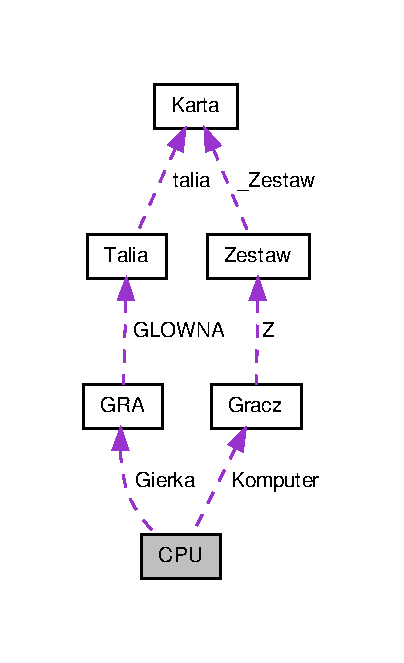
\includegraphics[width=194pt]{class_c_p_u__coll__graph}
\end{center}
\end{figure}
\subsection*{Metody publiczne}
\begin{DoxyCompactItemize}
\item 
void \hyperlink{class_c_p_u_aca73986a06413986e1569e81ae475913}{Wymiana} (\hyperlink{class_g_r_a}{G\-R\-A} \&Game)
\begin{DoxyCompactList}\small\item\em Metoda wymiany kart dla komputera.\-Jesli bd wymienial to co bd wymienial. \end{DoxyCompactList}\item 
\hyperlink{class_c_p_u_a2fdd8153d0979ccad9ed8452897267f4}{C\-P\-U} ()
\begin{DoxyCompactList}\small\item\em Inicjalizuje konstruktor. \end{DoxyCompactList}\item 
\hyperlink{class_c_p_u_ab5a7a17a7c732fda55456f2d929839cd}{C\-P\-U} (string nazwa)
\begin{DoxyCompactList}\small\item\em Metoda nadaje nazwe graczowi z komputera. \end{DoxyCompactList}\item 
void \hyperlink{class_c_p_u_a400f9910fc72454497684731380621bd}{Co\-Bedzie\-Wymienial} (\hyperlink{class_g_r_a}{G\-R\-A} \&Game)
\begin{DoxyCompactList}\small\item\em Metoda liczy uklad kart komputera i wywoluje odpowiednie funckje wymiany w zaleznosci od ukladu kart. \end{DoxyCompactList}\item 
void \hyperlink{class_c_p_u_a60fa4d2a96e91be88c4550505f6614ed}{Decyzja} (\hyperlink{class_g_r_a}{G\-R\-A} \&Game)
\begin{DoxyCompactList}\small\item\em Metoda odpowiadajaca za decyzje gracza \-: -\/podbija/czeka -\/przebija -\/pasuje. \end{DoxyCompactList}\item 
void \hyperlink{class_c_p_u_a6902858786d30ae35d2c7a3d9e29b0f5}{Decyzja\-Z\-Czekaniem} (\hyperlink{class_g_r_a}{G\-R\-A} \&Game)
\begin{DoxyCompactList}\small\item\em Metoda odpowiadajaca za decyzje gracza z czekaniem. \end{DoxyCompactList}\item 
char \hyperlink{class_c_p_u_a2d619927e12bcf71bbc30ad44ba3fada}{Co\-Obstawi} (\hyperlink{class_g_r_a}{G\-R\-A} \&Game)
\begin{DoxyCompactList}\small\item\em Metoda liczy uklad kart komputera i decyduje czy komputer bd pasowal,czekal czy podbijal. \end{DoxyCompactList}\end{DoxyCompactItemize}
\subsection*{Atrybuty publiczne}
\begin{DoxyCompactItemize}
\item 
\hyperlink{class_gracz}{Gracz} \hyperlink{class_c_p_u_a6530a4639d59e54a02ead99b6477f486}{Komputer}
\begin{DoxyCompactList}\small\item\em Tworzy obiekt typu \hyperlink{class_gracz}{Gracz}. \end{DoxyCompactList}\item 
\hyperlink{class_g_r_a}{G\-R\-A} \hyperlink{class_c_p_u_aaa02aad3d7238ef5d8908319c02836f0}{Gierka}
\begin{DoxyCompactList}\small\item\em Tworzy obiekt typu \hyperlink{class_g_r_a}{G\-R\-A}. \end{DoxyCompactList}\end{DoxyCompactItemize}
\subsection*{Metody prywatne}
\begin{DoxyCompactItemize}
\item 
bool \hyperlink{class_c_p_u_ae28436e9e40e05d897bcdc3f5f137de9}{Czy\-Bedzie\-Wymienial} (\hyperlink{class_g_r_a}{G\-R\-A} \&Game)
\begin{DoxyCompactList}\small\item\em Sprawdza czy komputer chce wymienic karty ze swojego zestawu. \end{DoxyCompactList}\item 
void \hyperlink{class_c_p_u_a9eeb4244b31bbdfb59c0ad7f9b51d0e6}{Wymiana\-Dla0} (\hyperlink{class_g_r_a}{G\-R\-A} \&Game)
\begin{DoxyCompactList}\small\item\em Metoda wymiany kart dla komputera z ukladem 0 ( nie ma par ,trojek ,fulla, strita itd.) \end{DoxyCompactList}\item 
void \hyperlink{class_c_p_u_a996ad643815fb962ffc60c543efdb4bd}{Wymiana\-Dla1} (\hyperlink{class_g_r_a}{G\-R\-A} \&Game)
\begin{DoxyCompactList}\small\item\em Metoda wymiany kart dla komputera z ukladem 1(czyli dla jednej pary) \end{DoxyCompactList}\item 
void \hyperlink{class_c_p_u_ae0c3f82d98dab6621d5a221b56e9cf94}{Wymiana\-Dla2} (\hyperlink{class_g_r_a}{G\-R\-A} \&Game)
\begin{DoxyCompactList}\small\item\em Metoda wymiany kart dla komputera z ukladem 2 (czyli dla dw�ch par) \end{DoxyCompactList}\item 
void \hyperlink{class_c_p_u_a173d904de6429cec82d21bc47260e73b}{Wymiana\-Dla3} (\hyperlink{class_g_r_a}{G\-R\-A} \&Game)
\begin{DoxyCompactList}\small\item\em Metoda wymiany kart dla komputera z ukladem 3(czyli dla trojki) \end{DoxyCompactList}\item 
void \hyperlink{class_c_p_u_ab07d6b432de3847e0b3e9f953e54dca1}{Wskazindeksy\-Slabych} (\hyperlink{class_gracz}{Gracz} ziomek, vector$<$ int $>$ \&slabe)
\begin{DoxyCompactList}\small\item\em Metoda wskazuje indeksy slabych kart. \end{DoxyCompactList}\end{DoxyCompactItemize}
\subsection*{Atrybuty prywatne}
\begin{DoxyCompactItemize}
\item 
int \hyperlink{class_c_p_u_a1e17b85bb84e5e60c45334ea8e409690}{random}
\begin{DoxyCompactList}\small\item\em Zmienna pomocnicza typu int. \end{DoxyCompactList}\item 
int \hyperlink{class_c_p_u_a239c611d8bcd010f2b2676f22afb12d8}{iter}
\begin{DoxyCompactList}\small\item\em Zmienna pomocnicza typu int. \end{DoxyCompactList}\item 
bool \hyperlink{class_c_p_u_aff66a069827189be5f8c64d32dc1c9d5}{p1}
\begin{DoxyCompactList}\small\item\em Zmienne pomocnicze. \end{DoxyCompactList}\item 
bool \hyperlink{class_c_p_u_a7c30767fcadc9d443d4c591c5ea9f905}{p2}
\item 
bool \hyperlink{class_c_p_u_a10840329e8aaacd30333e5ff973d0abc}{p3}
\end{DoxyCompactItemize}


\subsection{Opis szczegółowy}
Klasa modeluje pojecie cpu czyli gracza komputerowego. 

Definicja w linii 18 pliku C\-P\-U.\-h.



\subsection{Dokumentacja konstruktora i destruktora}
\hypertarget{class_c_p_u_a2fdd8153d0979ccad9ed8452897267f4}{\index{C\-P\-U@{C\-P\-U}!C\-P\-U@{C\-P\-U}}
\index{C\-P\-U@{C\-P\-U}!CPU@{C\-P\-U}}
\subsubsection[{C\-P\-U}]{\setlength{\rightskip}{0pt plus 5cm}C\-P\-U\-::\-C\-P\-U (
\begin{DoxyParamCaption}
{}
\end{DoxyParamCaption}
)}}\label{class_c_p_u_a2fdd8153d0979ccad9ed8452897267f4}


Definicja w linii 37 pliku C\-P\-U.\-cpp.

\hypertarget{class_c_p_u_ab5a7a17a7c732fda55456f2d929839cd}{\index{C\-P\-U@{C\-P\-U}!C\-P\-U@{C\-P\-U}}
\index{C\-P\-U@{C\-P\-U}!CPU@{C\-P\-U}}
\subsubsection[{C\-P\-U}]{\setlength{\rightskip}{0pt plus 5cm}C\-P\-U\-::\-C\-P\-U (
\begin{DoxyParamCaption}
\item[{string}]{nazwa}
\end{DoxyParamCaption}
)}}\label{class_c_p_u_ab5a7a17a7c732fda55456f2d929839cd}


Definicja w linii 27 pliku C\-P\-U.\-cpp.



\subsection{Dokumentacja funkcji składowych}
\hypertarget{class_c_p_u_a400f9910fc72454497684731380621bd}{\index{C\-P\-U@{C\-P\-U}!Co\-Bedzie\-Wymienial@{Co\-Bedzie\-Wymienial}}
\index{Co\-Bedzie\-Wymienial@{Co\-Bedzie\-Wymienial}!CPU@{C\-P\-U}}
\subsubsection[{Co\-Bedzie\-Wymienial}]{\setlength{\rightskip}{0pt plus 5cm}void C\-P\-U\-::\-Co\-Bedzie\-Wymienial (
\begin{DoxyParamCaption}
\item[{{\bf G\-R\-A} \&}]{Game}
\end{DoxyParamCaption}
)}}\label{class_c_p_u_a400f9910fc72454497684731380621bd}


Definicja w linii 58 pliku C\-P\-U.\-cpp.



Oto graf wywołań dla tej funkcji\-:\nopagebreak
\begin{figure}[H]
\begin{center}
\leavevmode
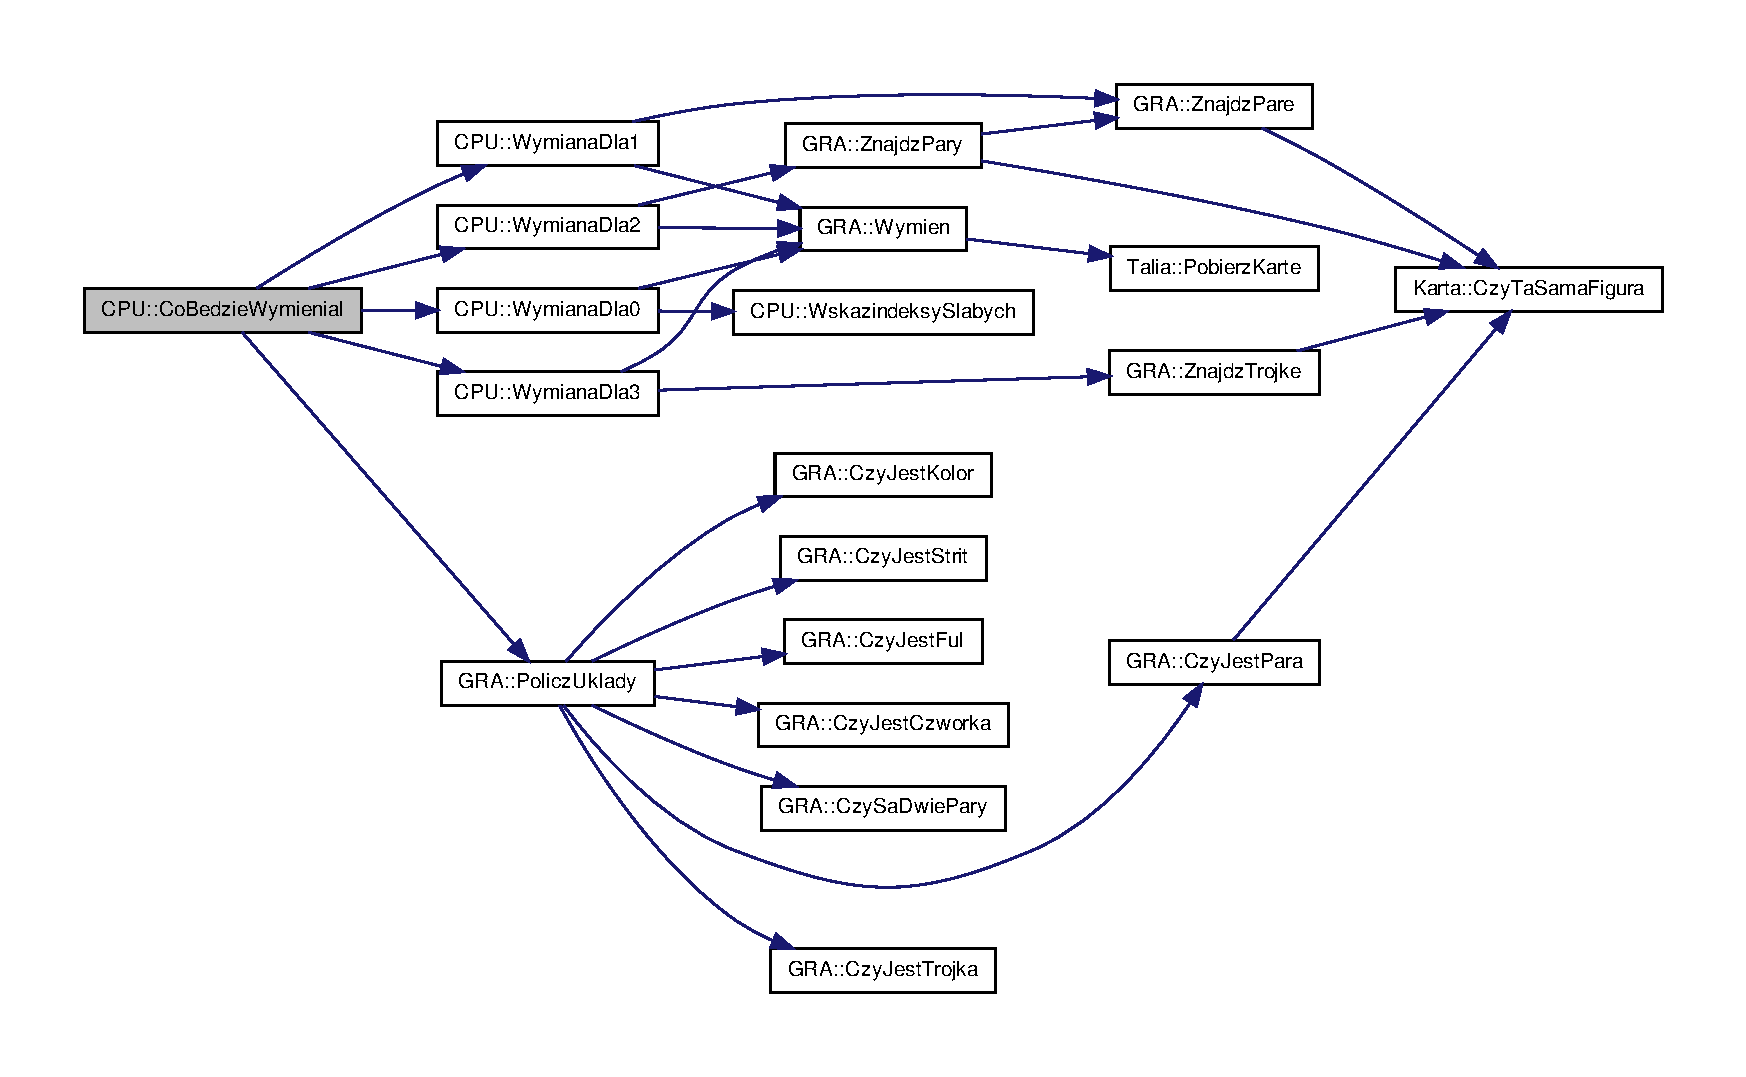
\includegraphics[width=350pt]{class_c_p_u_a400f9910fc72454497684731380621bd_cgraph}
\end{center}
\end{figure}




Oto graf wywoływań tej funkcji\-:
\nopagebreak
\begin{figure}[H]
\begin{center}
\leavevmode
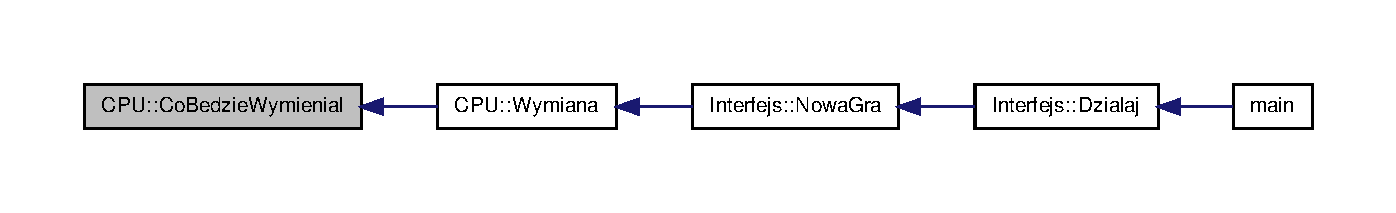
\includegraphics[width=350pt]{class_c_p_u_a400f9910fc72454497684731380621bd_icgraph}
\end{center}
\end{figure}


\hypertarget{class_c_p_u_a2d619927e12bcf71bbc30ad44ba3fada}{\index{C\-P\-U@{C\-P\-U}!Co\-Obstawi@{Co\-Obstawi}}
\index{Co\-Obstawi@{Co\-Obstawi}!CPU@{C\-P\-U}}
\subsubsection[{Co\-Obstawi}]{\setlength{\rightskip}{0pt plus 5cm}char C\-P\-U\-::\-Co\-Obstawi (
\begin{DoxyParamCaption}
\item[{{\bf G\-R\-A} \&}]{Game}
\end{DoxyParamCaption}
)}}\label{class_c_p_u_a2d619927e12bcf71bbc30ad44ba3fada}


Definicja w linii 274 pliku C\-P\-U.\-cpp.



Oto graf wywołań dla tej funkcji\-:
\nopagebreak
\begin{figure}[H]
\begin{center}
\leavevmode
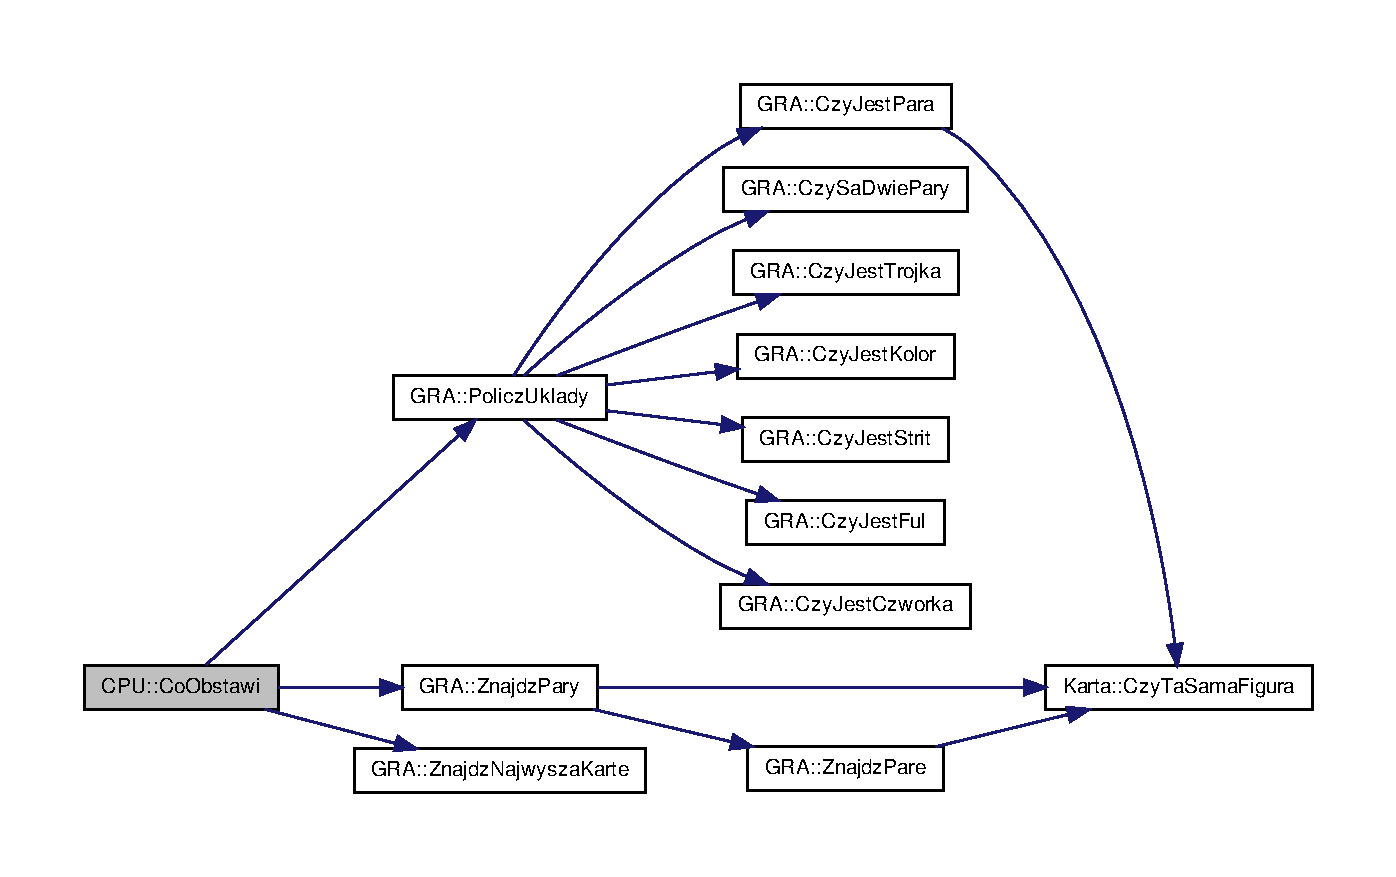
\includegraphics[width=350pt]{class_c_p_u_a2d619927e12bcf71bbc30ad44ba3fada_cgraph}
\end{center}
\end{figure}




Oto graf wywoływań tej funkcji\-:
\nopagebreak
\begin{figure}[H]
\begin{center}
\leavevmode
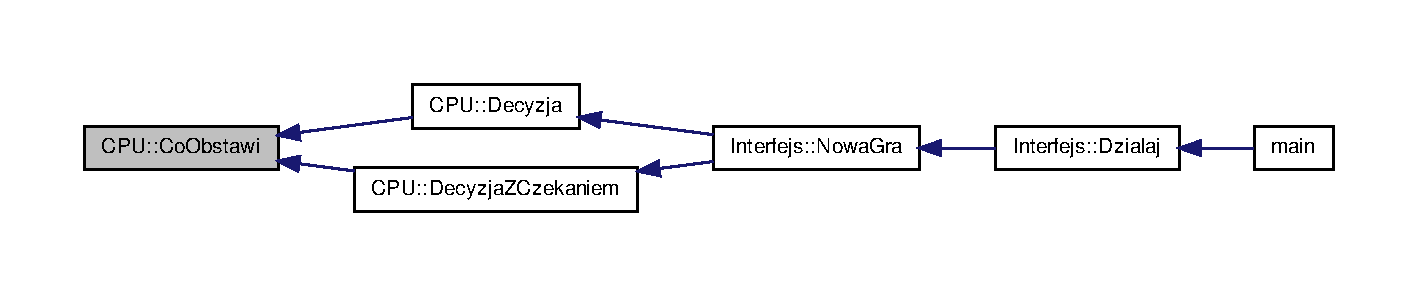
\includegraphics[width=350pt]{class_c_p_u_a2d619927e12bcf71bbc30ad44ba3fada_icgraph}
\end{center}
\end{figure}


\hypertarget{class_c_p_u_ae28436e9e40e05d897bcdc3f5f137de9}{\index{C\-P\-U@{C\-P\-U}!Czy\-Bedzie\-Wymienial@{Czy\-Bedzie\-Wymienial}}
\index{Czy\-Bedzie\-Wymienial@{Czy\-Bedzie\-Wymienial}!CPU@{C\-P\-U}}
\subsubsection[{Czy\-Bedzie\-Wymienial}]{\setlength{\rightskip}{0pt plus 5cm}bool C\-P\-U\-::\-Czy\-Bedzie\-Wymienial (
\begin{DoxyParamCaption}
\item[{{\bf G\-R\-A} \&}]{Game}
\end{DoxyParamCaption}
)\hspace{0.3cm}{\ttfamily [private]}}}\label{class_c_p_u_ae28436e9e40e05d897bcdc3f5f137de9}
\begin{DoxyReturn}{Zwraca}
Zwraca true lub false. 
\end{DoxyReturn}


Definicja w linii 9 pliku C\-P\-U.\-cpp.



Oto graf wywołań dla tej funkcji\-:\nopagebreak
\begin{figure}[H]
\begin{center}
\leavevmode
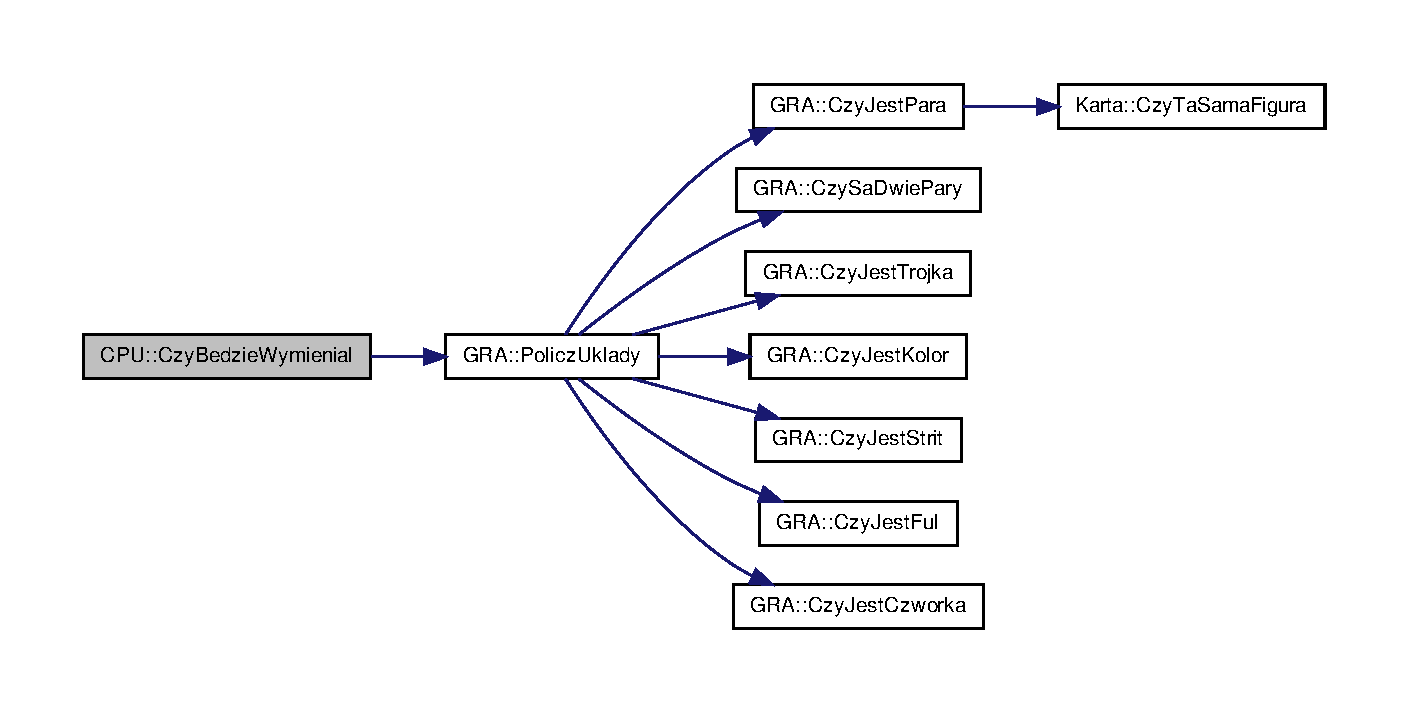
\includegraphics[width=350pt]{class_c_p_u_ae28436e9e40e05d897bcdc3f5f137de9_cgraph}
\end{center}
\end{figure}




Oto graf wywoływań tej funkcji\-:
\nopagebreak
\begin{figure}[H]
\begin{center}
\leavevmode
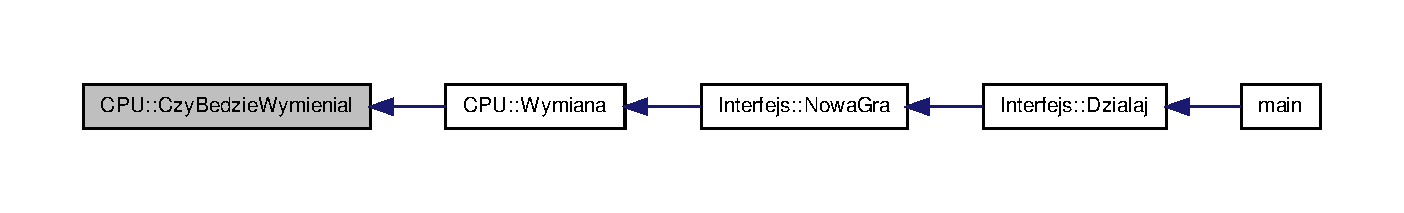
\includegraphics[width=350pt]{class_c_p_u_ae28436e9e40e05d897bcdc3f5f137de9_icgraph}
\end{center}
\end{figure}


\hypertarget{class_c_p_u_a60fa4d2a96e91be88c4550505f6614ed}{\index{C\-P\-U@{C\-P\-U}!Decyzja@{Decyzja}}
\index{Decyzja@{Decyzja}!CPU@{C\-P\-U}}
\subsubsection[{Decyzja}]{\setlength{\rightskip}{0pt plus 5cm}void C\-P\-U\-::\-Decyzja (
\begin{DoxyParamCaption}
\item[{{\bf G\-R\-A} \&}]{Game}
\end{DoxyParamCaption}
)}}\label{class_c_p_u_a60fa4d2a96e91be88c4550505f6614ed}


Definicja w linii 196 pliku C\-P\-U.\-cpp.



Oto graf wywołań dla tej funkcji\-:
\nopagebreak
\begin{figure}[H]
\begin{center}
\leavevmode
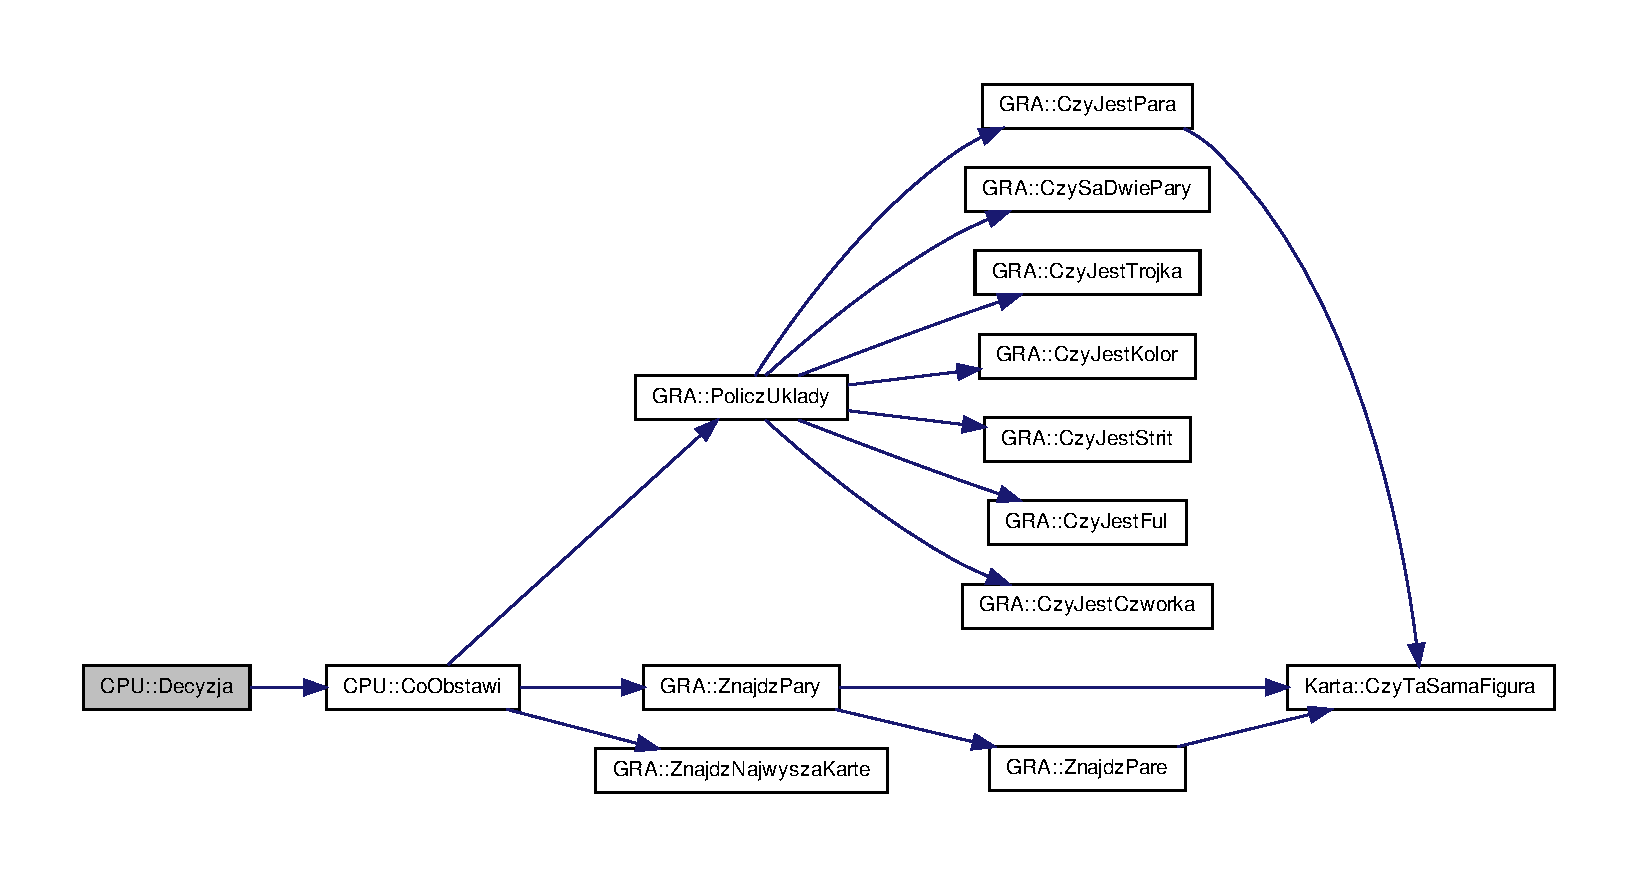
\includegraphics[width=350pt]{class_c_p_u_a60fa4d2a96e91be88c4550505f6614ed_cgraph}
\end{center}
\end{figure}




Oto graf wywoływań tej funkcji\-:
\nopagebreak
\begin{figure}[H]
\begin{center}
\leavevmode
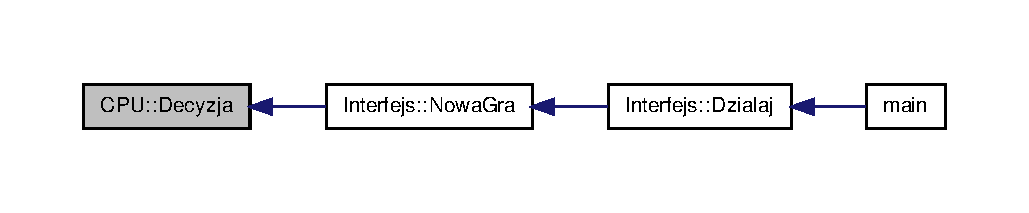
\includegraphics[width=350pt]{class_c_p_u_a60fa4d2a96e91be88c4550505f6614ed_icgraph}
\end{center}
\end{figure}


\hypertarget{class_c_p_u_a6902858786d30ae35d2c7a3d9e29b0f5}{\index{C\-P\-U@{C\-P\-U}!Decyzja\-Z\-Czekaniem@{Decyzja\-Z\-Czekaniem}}
\index{Decyzja\-Z\-Czekaniem@{Decyzja\-Z\-Czekaniem}!CPU@{C\-P\-U}}
\subsubsection[{Decyzja\-Z\-Czekaniem}]{\setlength{\rightskip}{0pt plus 5cm}void C\-P\-U\-::\-Decyzja\-Z\-Czekaniem (
\begin{DoxyParamCaption}
\item[{{\bf G\-R\-A} \&}]{Game}
\end{DoxyParamCaption}
)}}\label{class_c_p_u_a6902858786d30ae35d2c7a3d9e29b0f5}


Definicja w linii 311 pliku C\-P\-U.\-cpp.



Oto graf wywołań dla tej funkcji\-:
\nopagebreak
\begin{figure}[H]
\begin{center}
\leavevmode
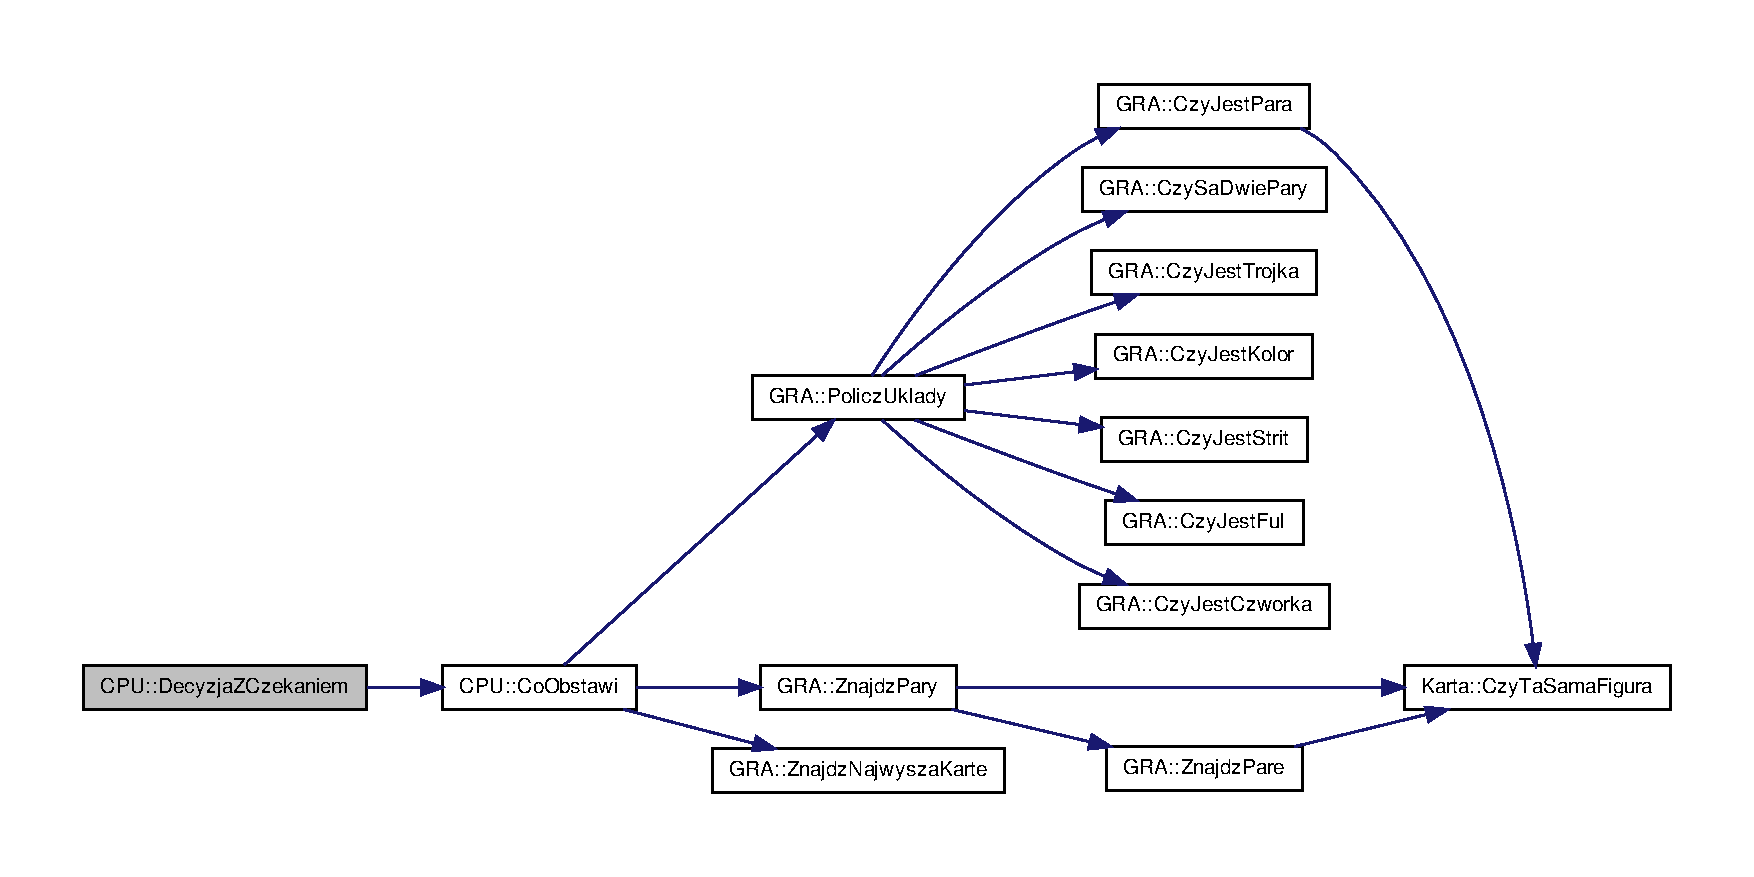
\includegraphics[width=350pt]{class_c_p_u_a6902858786d30ae35d2c7a3d9e29b0f5_cgraph}
\end{center}
\end{figure}




Oto graf wywoływań tej funkcji\-:
\nopagebreak
\begin{figure}[H]
\begin{center}
\leavevmode
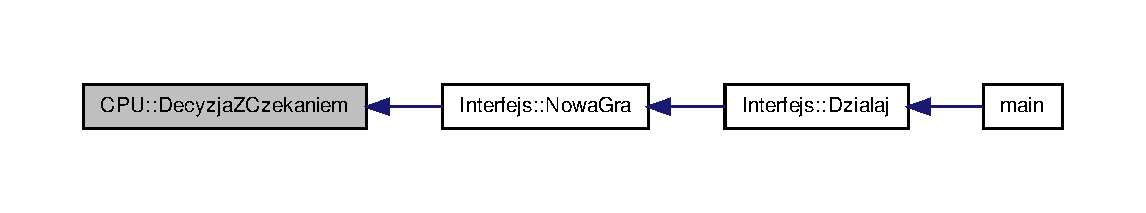
\includegraphics[width=350pt]{class_c_p_u_a6902858786d30ae35d2c7a3d9e29b0f5_icgraph}
\end{center}
\end{figure}


\hypertarget{class_c_p_u_ab07d6b432de3847e0b3e9f953e54dca1}{\index{C\-P\-U@{C\-P\-U}!Wskazindeksy\-Slabych@{Wskazindeksy\-Slabych}}
\index{Wskazindeksy\-Slabych@{Wskazindeksy\-Slabych}!CPU@{C\-P\-U}}
\subsubsection[{Wskazindeksy\-Slabych}]{\setlength{\rightskip}{0pt plus 5cm}void C\-P\-U\-::\-Wskazindeksy\-Slabych (
\begin{DoxyParamCaption}
\item[{{\bf Gracz}}]{ziomek, }
\item[{vector$<$ int $>$ \&}]{slabe}
\end{DoxyParamCaption}
)\hspace{0.3cm}{\ttfamily [private]}}}\label{class_c_p_u_ab07d6b432de3847e0b3e9f953e54dca1}


Definicja w linii 134 pliku C\-P\-U.\-cpp.



Oto graf wywoływań tej funkcji\-:
\nopagebreak
\begin{figure}[H]
\begin{center}
\leavevmode
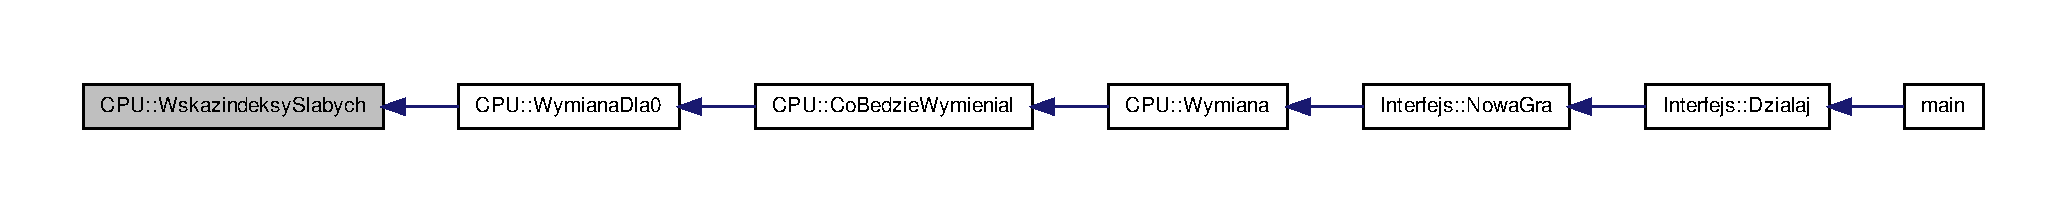
\includegraphics[width=350pt]{class_c_p_u_ab07d6b432de3847e0b3e9f953e54dca1_icgraph}
\end{center}
\end{figure}


\hypertarget{class_c_p_u_aca73986a06413986e1569e81ae475913}{\index{C\-P\-U@{C\-P\-U}!Wymiana@{Wymiana}}
\index{Wymiana@{Wymiana}!CPU@{C\-P\-U}}
\subsubsection[{Wymiana}]{\setlength{\rightskip}{0pt plus 5cm}void C\-P\-U\-::\-Wymiana (
\begin{DoxyParamCaption}
\item[{{\bf G\-R\-A} \&}]{Game}
\end{DoxyParamCaption}
)}}\label{class_c_p_u_aca73986a06413986e1569e81ae475913}


Definicja w linii 46 pliku C\-P\-U.\-cpp.



Oto graf wywołań dla tej funkcji\-:\nopagebreak
\begin{figure}[H]
\begin{center}
\leavevmode
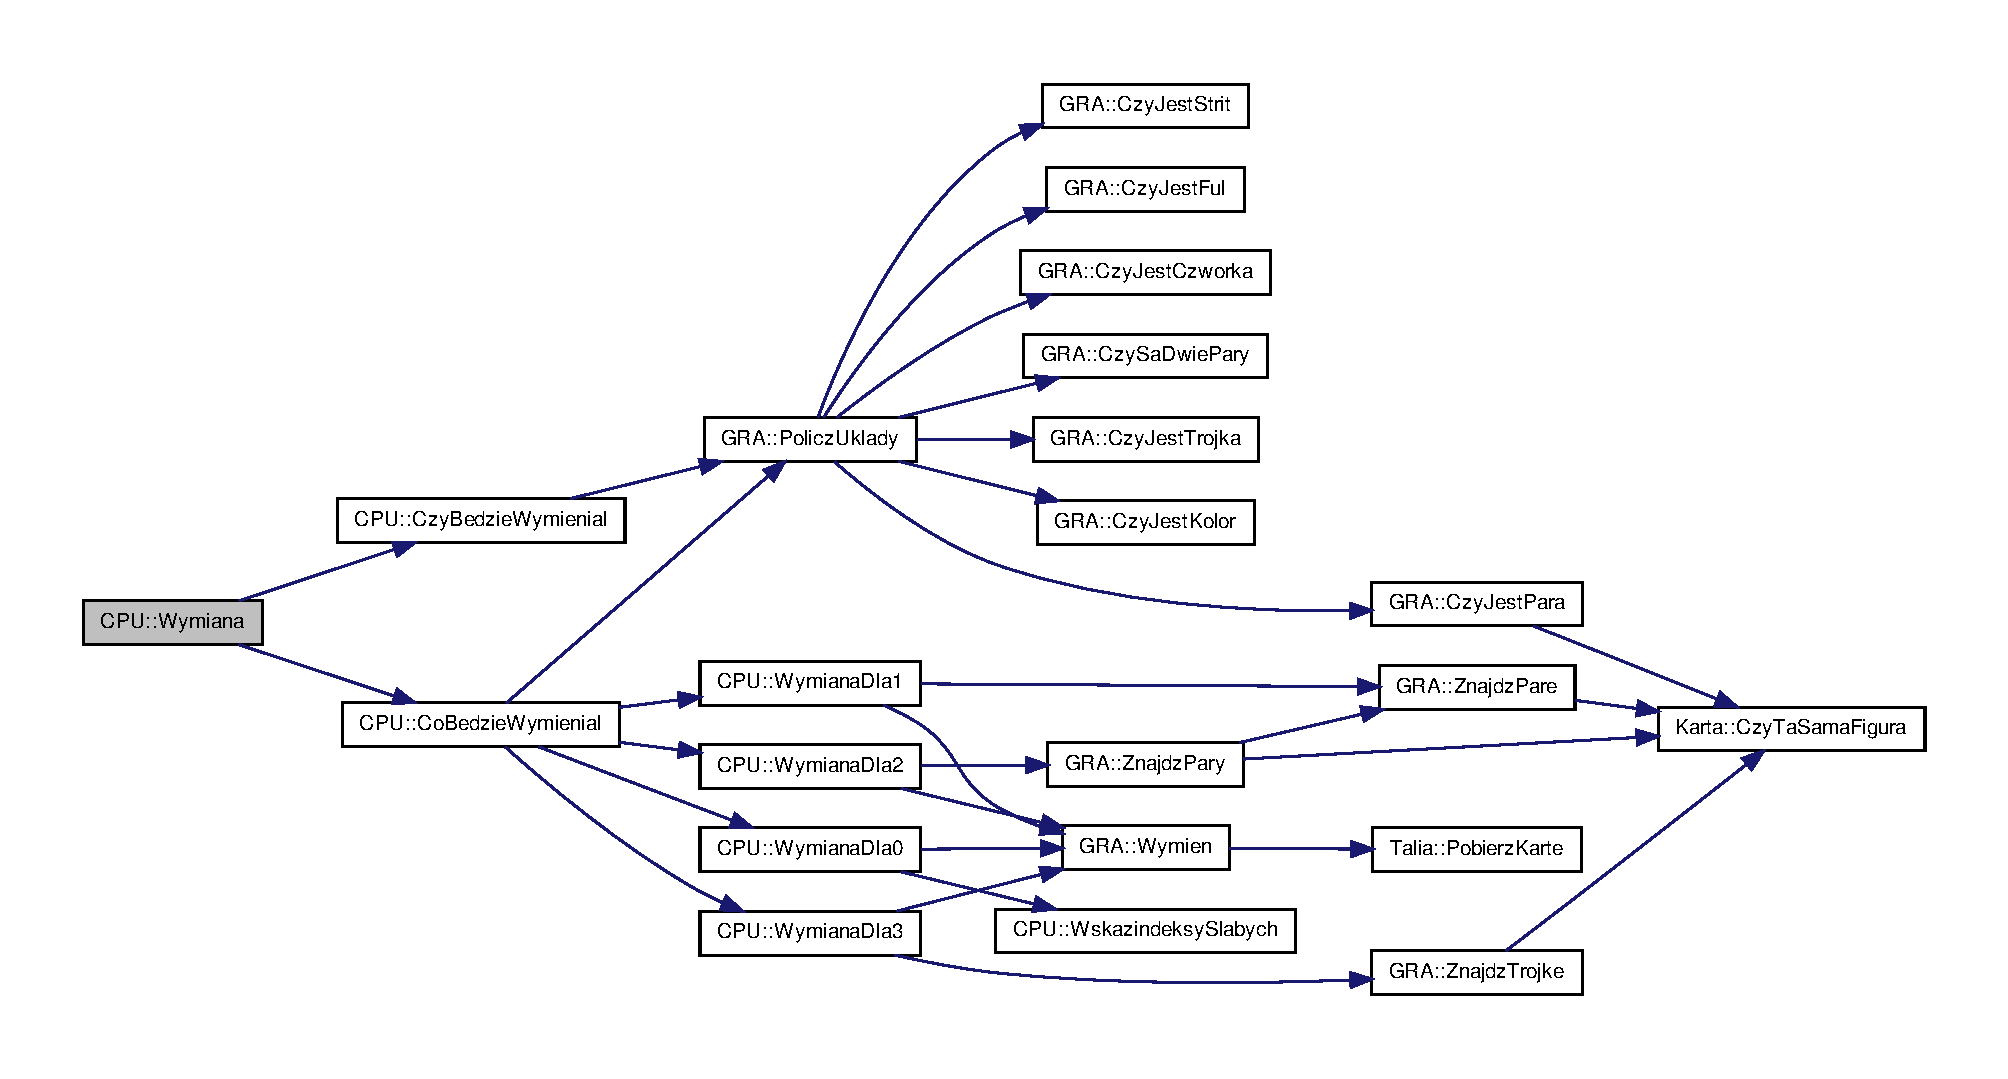
\includegraphics[width=350pt]{class_c_p_u_aca73986a06413986e1569e81ae475913_cgraph}
\end{center}
\end{figure}




Oto graf wywoływań tej funkcji\-:
\nopagebreak
\begin{figure}[H]
\begin{center}
\leavevmode
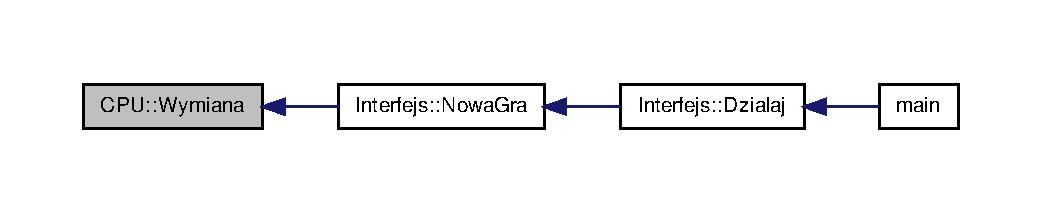
\includegraphics[width=350pt]{class_c_p_u_aca73986a06413986e1569e81ae475913_icgraph}
\end{center}
\end{figure}


\hypertarget{class_c_p_u_a9eeb4244b31bbdfb59c0ad7f9b51d0e6}{\index{C\-P\-U@{C\-P\-U}!Wymiana\-Dla0@{Wymiana\-Dla0}}
\index{Wymiana\-Dla0@{Wymiana\-Dla0}!CPU@{C\-P\-U}}
\subsubsection[{Wymiana\-Dla0}]{\setlength{\rightskip}{0pt plus 5cm}void C\-P\-U\-::\-Wymiana\-Dla0 (
\begin{DoxyParamCaption}
\item[{{\bf G\-R\-A} \&}]{Game}
\end{DoxyParamCaption}
)\hspace{0.3cm}{\ttfamily [private]}}}\label{class_c_p_u_a9eeb4244b31bbdfb59c0ad7f9b51d0e6}


Definicja w linii 120 pliku C\-P\-U.\-cpp.



Oto graf wywołań dla tej funkcji\-:\nopagebreak
\begin{figure}[H]
\begin{center}
\leavevmode
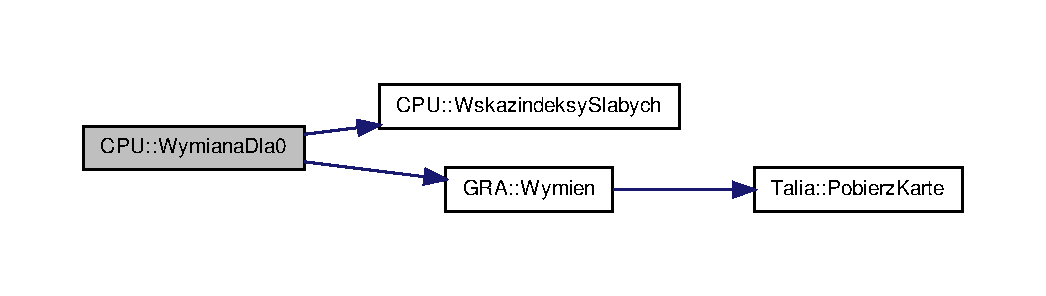
\includegraphics[width=350pt]{class_c_p_u_a9eeb4244b31bbdfb59c0ad7f9b51d0e6_cgraph}
\end{center}
\end{figure}




Oto graf wywoływań tej funkcji\-:
\nopagebreak
\begin{figure}[H]
\begin{center}
\leavevmode
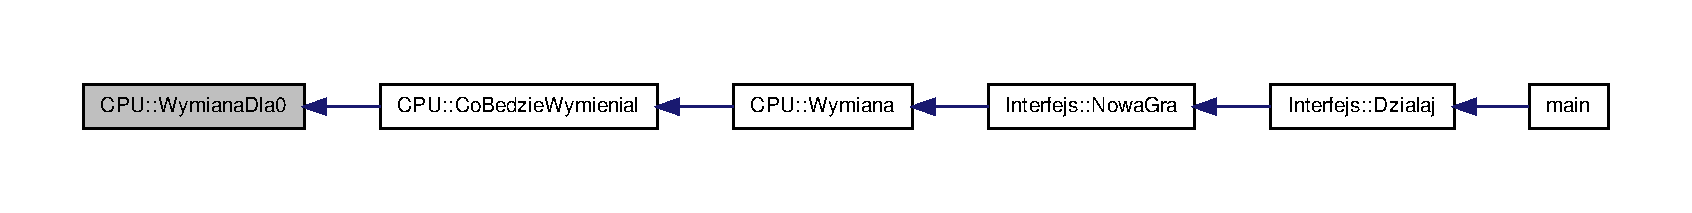
\includegraphics[width=350pt]{class_c_p_u_a9eeb4244b31bbdfb59c0ad7f9b51d0e6_icgraph}
\end{center}
\end{figure}


\hypertarget{class_c_p_u_a996ad643815fb962ffc60c543efdb4bd}{\index{C\-P\-U@{C\-P\-U}!Wymiana\-Dla1@{Wymiana\-Dla1}}
\index{Wymiana\-Dla1@{Wymiana\-Dla1}!CPU@{C\-P\-U}}
\subsubsection[{Wymiana\-Dla1}]{\setlength{\rightskip}{0pt plus 5cm}void C\-P\-U\-::\-Wymiana\-Dla1 (
\begin{DoxyParamCaption}
\item[{{\bf G\-R\-A} \&}]{Game}
\end{DoxyParamCaption}
)\hspace{0.3cm}{\ttfamily [private]}}}\label{class_c_p_u_a996ad643815fb962ffc60c543efdb4bd}


Definicja w linii 148 pliku C\-P\-U.\-cpp.



Oto graf wywołań dla tej funkcji\-:\nopagebreak
\begin{figure}[H]
\begin{center}
\leavevmode
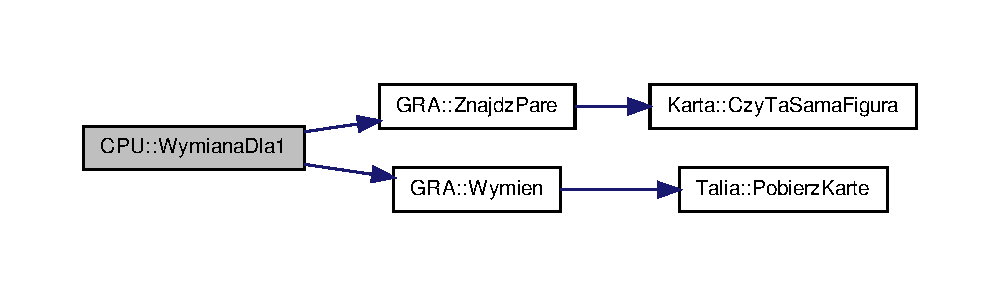
\includegraphics[width=350pt]{class_c_p_u_a996ad643815fb962ffc60c543efdb4bd_cgraph}
\end{center}
\end{figure}




Oto graf wywoływań tej funkcji\-:
\nopagebreak
\begin{figure}[H]
\begin{center}
\leavevmode
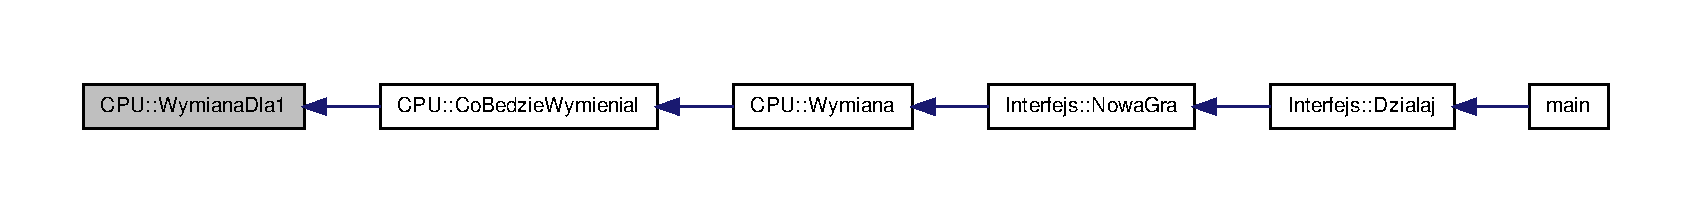
\includegraphics[width=350pt]{class_c_p_u_a996ad643815fb962ffc60c543efdb4bd_icgraph}
\end{center}
\end{figure}


\hypertarget{class_c_p_u_ae0c3f82d98dab6621d5a221b56e9cf94}{\index{C\-P\-U@{C\-P\-U}!Wymiana\-Dla2@{Wymiana\-Dla2}}
\index{Wymiana\-Dla2@{Wymiana\-Dla2}!CPU@{C\-P\-U}}
\subsubsection[{Wymiana\-Dla2}]{\setlength{\rightskip}{0pt plus 5cm}void C\-P\-U\-::\-Wymiana\-Dla2 (
\begin{DoxyParamCaption}
\item[{{\bf G\-R\-A} \&}]{Game}
\end{DoxyParamCaption}
)\hspace{0.3cm}{\ttfamily [private]}}}\label{class_c_p_u_ae0c3f82d98dab6621d5a221b56e9cf94}


Definicja w linii 168 pliku C\-P\-U.\-cpp.



Oto graf wywołań dla tej funkcji\-:\nopagebreak
\begin{figure}[H]
\begin{center}
\leavevmode
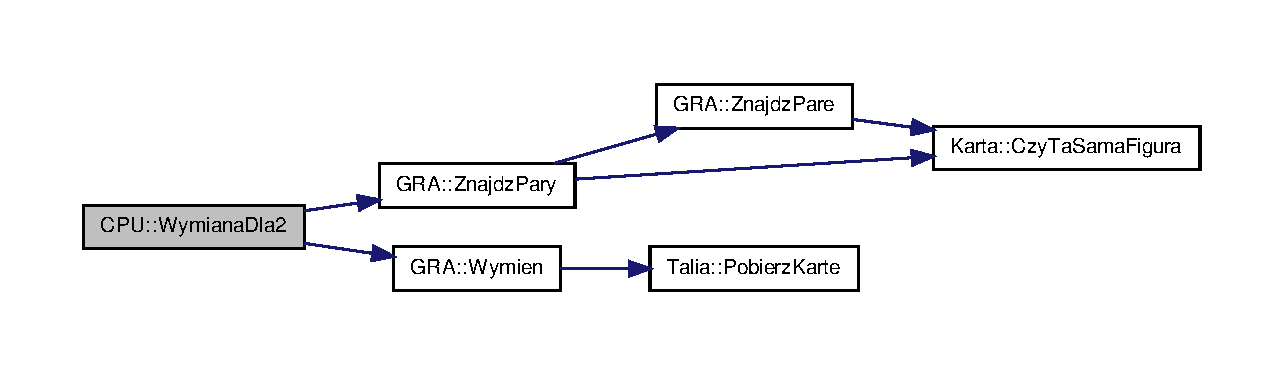
\includegraphics[width=350pt]{class_c_p_u_ae0c3f82d98dab6621d5a221b56e9cf94_cgraph}
\end{center}
\end{figure}




Oto graf wywoływań tej funkcji\-:
\nopagebreak
\begin{figure}[H]
\begin{center}
\leavevmode
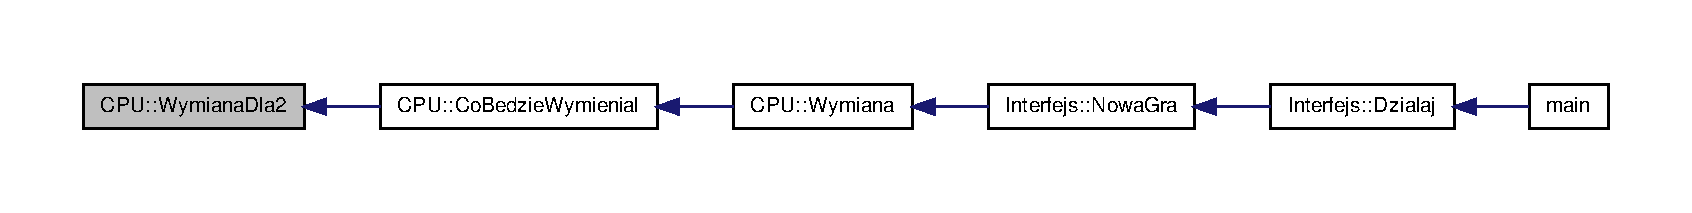
\includegraphics[width=350pt]{class_c_p_u_ae0c3f82d98dab6621d5a221b56e9cf94_icgraph}
\end{center}
\end{figure}


\hypertarget{class_c_p_u_a173d904de6429cec82d21bc47260e73b}{\index{C\-P\-U@{C\-P\-U}!Wymiana\-Dla3@{Wymiana\-Dla3}}
\index{Wymiana\-Dla3@{Wymiana\-Dla3}!CPU@{C\-P\-U}}
\subsubsection[{Wymiana\-Dla3}]{\setlength{\rightskip}{0pt plus 5cm}void C\-P\-U\-::\-Wymiana\-Dla3 (
\begin{DoxyParamCaption}
\item[{{\bf G\-R\-A} \&}]{Game}
\end{DoxyParamCaption}
)\hspace{0.3cm}{\ttfamily [private]}}}\label{class_c_p_u_a173d904de6429cec82d21bc47260e73b}


Definicja w linii 182 pliku C\-P\-U.\-cpp.



Oto graf wywołań dla tej funkcji\-:\nopagebreak
\begin{figure}[H]
\begin{center}
\leavevmode
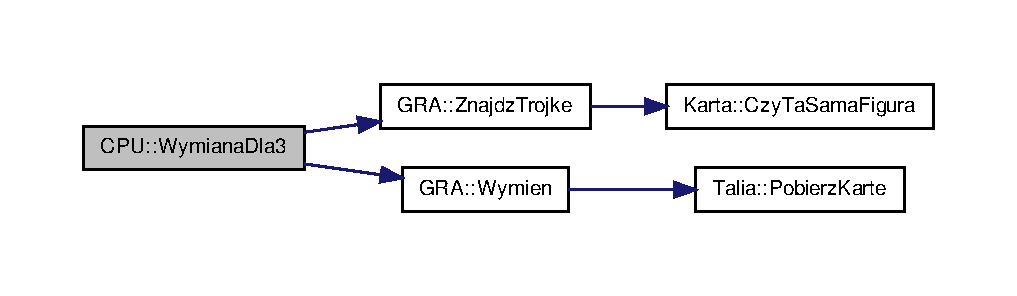
\includegraphics[width=350pt]{class_c_p_u_a173d904de6429cec82d21bc47260e73b_cgraph}
\end{center}
\end{figure}




Oto graf wywoływań tej funkcji\-:
\nopagebreak
\begin{figure}[H]
\begin{center}
\leavevmode
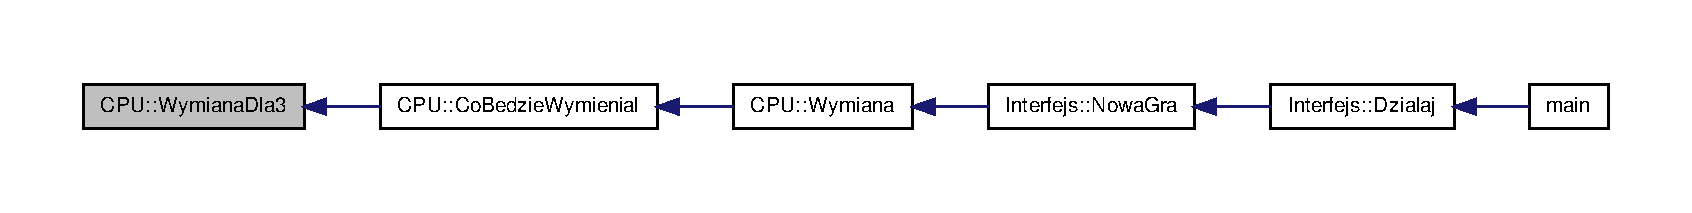
\includegraphics[width=350pt]{class_c_p_u_a173d904de6429cec82d21bc47260e73b_icgraph}
\end{center}
\end{figure}




\subsection{Dokumentacja atrybutów składowych}
\hypertarget{class_c_p_u_aaa02aad3d7238ef5d8908319c02836f0}{\index{C\-P\-U@{C\-P\-U}!Gierka@{Gierka}}
\index{Gierka@{Gierka}!CPU@{C\-P\-U}}
\subsubsection[{Gierka}]{\setlength{\rightskip}{0pt plus 5cm}{\bf G\-R\-A} C\-P\-U\-::\-Gierka}}\label{class_c_p_u_aaa02aad3d7238ef5d8908319c02836f0}


Definicja w linii 81 pliku C\-P\-U.\-h.

\hypertarget{class_c_p_u_a239c611d8bcd010f2b2676f22afb12d8}{\index{C\-P\-U@{C\-P\-U}!iter@{iter}}
\index{iter@{iter}!CPU@{C\-P\-U}}
\subsubsection[{iter}]{\setlength{\rightskip}{0pt plus 5cm}int C\-P\-U\-::iter\hspace{0.3cm}{\ttfamily [private]}}}\label{class_c_p_u_a239c611d8bcd010f2b2676f22afb12d8}


Definicja w linii 55 pliku C\-P\-U.\-h.

\hypertarget{class_c_p_u_a6530a4639d59e54a02ead99b6477f486}{\index{C\-P\-U@{C\-P\-U}!Komputer@{Komputer}}
\index{Komputer@{Komputer}!CPU@{C\-P\-U}}
\subsubsection[{Komputer}]{\setlength{\rightskip}{0pt plus 5cm}{\bf Gracz} C\-P\-U\-::\-Komputer}}\label{class_c_p_u_a6530a4639d59e54a02ead99b6477f486}


Definicja w linii 77 pliku C\-P\-U.\-h.

\hypertarget{class_c_p_u_aff66a069827189be5f8c64d32dc1c9d5}{\index{C\-P\-U@{C\-P\-U}!p1@{p1}}
\index{p1@{p1}!CPU@{C\-P\-U}}
\subsubsection[{p1}]{\setlength{\rightskip}{0pt plus 5cm}bool C\-P\-U\-::p1\hspace{0.3cm}{\ttfamily [private]}}}\label{class_c_p_u_aff66a069827189be5f8c64d32dc1c9d5}
\begin{DoxyReturn}{Zwraca}
Zwracaja false lub true. 
\end{DoxyReturn}


Definicja w linii 60 pliku C\-P\-U.\-h.

\hypertarget{class_c_p_u_a7c30767fcadc9d443d4c591c5ea9f905}{\index{C\-P\-U@{C\-P\-U}!p2@{p2}}
\index{p2@{p2}!CPU@{C\-P\-U}}
\subsubsection[{p2}]{\setlength{\rightskip}{0pt plus 5cm}bool C\-P\-U\-::p2\hspace{0.3cm}{\ttfamily [private]}}}\label{class_c_p_u_a7c30767fcadc9d443d4c591c5ea9f905}


Definicja w linii 60 pliku C\-P\-U.\-h.

\hypertarget{class_c_p_u_a10840329e8aaacd30333e5ff973d0abc}{\index{C\-P\-U@{C\-P\-U}!p3@{p3}}
\index{p3@{p3}!CPU@{C\-P\-U}}
\subsubsection[{p3}]{\setlength{\rightskip}{0pt plus 5cm}bool C\-P\-U\-::p3\hspace{0.3cm}{\ttfamily [private]}}}\label{class_c_p_u_a10840329e8aaacd30333e5ff973d0abc}


Definicja w linii 60 pliku C\-P\-U.\-h.

\hypertarget{class_c_p_u_a1e17b85bb84e5e60c45334ea8e409690}{\index{C\-P\-U@{C\-P\-U}!random@{random}}
\index{random@{random}!CPU@{C\-P\-U}}
\subsubsection[{random}]{\setlength{\rightskip}{0pt plus 5cm}int C\-P\-U\-::random\hspace{0.3cm}{\ttfamily [private]}}}\label{class_c_p_u_a1e17b85bb84e5e60c45334ea8e409690}


Definicja w linii 50 pliku C\-P\-U.\-h.



Dokumentacja dla tej klasy została wygenerowana z plików\-:\begin{DoxyCompactItemize}
\item 
/home/karolina/\-Pulpit/\-Project41\-Poker(1)/\-Project41\-Poker/\-Project41\-Poker/prj/inc/\hyperlink{_c_p_u_8h}{C\-P\-U.\-h}\item 
/home/karolina/\-Pulpit/\-Project41\-Poker(1)/\-Project41\-Poker/\-Project41\-Poker/prj/src/\hyperlink{_c_p_u_8cpp}{C\-P\-U.\-cpp}\end{DoxyCompactItemize}

\hypertarget{class_g_r_a}{\section{Dokumentacja klasy G\-R\-A}
\label{class_g_r_a}\index{G\-R\-A@{G\-R\-A}}
}


Modeluje pojecie \hyperlink{class_g_r_a}{G\-R\-A}.  




{\ttfamily \#include $<$G\-R\-A.\-h$>$}



Diagram współpracy dla G\-R\-A\-:\nopagebreak
\begin{figure}[H]
\begin{center}
\leavevmode
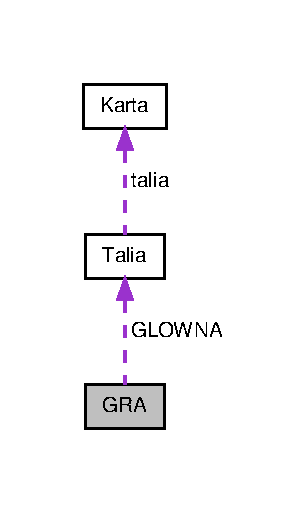
\includegraphics[width=148pt]{class_g_r_a__coll__graph}
\end{center}
\end{figure}
\subsection*{Metody publiczne}
\begin{DoxyCompactItemize}
\item 
\hyperlink{class_g_r_a_a267a2409e7b7144922b2f058fd6e2724}{G\-R\-A} ()
\begin{DoxyCompactList}\small\item\em Inicjalizuje konstruktor. \end{DoxyCompactList}\item 
int \hyperlink{class_g_r_a_a2f160ac8a217e52308423ddc950488d5}{Znajdz\-Pare} (\hyperlink{class_gracz}{Gracz} ziomek)
\begin{DoxyCompactList}\small\item\em Metoda szuka pary w zestawie kart gracza. \end{DoxyCompactList}\item 
vector$<$ int $>$ \hyperlink{class_g_r_a_a532c7c083060d7c846ac159b1f5c3f81}{Znajdz\-Pary} (\hyperlink{class_gracz}{Gracz} ziomek)
\begin{DoxyCompactList}\small\item\em Metoda szuka pary w zestawie kart gracza. \end{DoxyCompactList}\item 
int \hyperlink{class_g_r_a_a1045d31987634f497e342a4485c7db7b}{Znajdz\-Trojke} (\hyperlink{class_gracz}{Gracz} ziomek)
\begin{DoxyCompactList}\small\item\em Metoda znajduje trojke w zestawie kart gracza. \end{DoxyCompactList}\item 
bool \hyperlink{class_g_r_a_a7c72639bade47c93f59e4d02344b29de}{Czy\-Jest\-Para} (\hyperlink{class_gracz}{Gracz} ziomek)
\begin{DoxyCompactList}\small\item\em Metoda sprawdza czy jest para w zestawie kart gracza. \end{DoxyCompactList}\item 
bool \hyperlink{class_g_r_a_a83ff1a2e629b7368180f5ac0cc06fcfd}{Czy\-Sa\-Dwie\-Pary} (\hyperlink{class_gracz}{Gracz} ziomek)
\begin{DoxyCompactList}\small\item\em Metoda sprawdza czy sa dwie pary w zestawie kart gracza. \end{DoxyCompactList}\item 
bool \hyperlink{class_g_r_a_ab62696649e029ba3adc5876dee3c8fbc}{Czy\-Jest\-Trojka} (\hyperlink{class_gracz}{Gracz} ziomek)
\begin{DoxyCompactList}\small\item\em Metoda sprawdza czy jest trojka w zestawie kart gracza. \end{DoxyCompactList}\item 
bool \hyperlink{class_g_r_a_a3fb6dbd37229ac58c84a0b4f5403a3d6}{Czy\-Jest\-Strit} (\hyperlink{class_gracz}{Gracz} ziomek)
\begin{DoxyCompactList}\small\item\em Metoda sprawdza czy jest strit w zestawie kart gracza. \end{DoxyCompactList}\item 
bool \hyperlink{class_g_r_a_a04dd210d0146656fd70e2d10ccdf0065}{Czy\-Jest\-Kolor} (\hyperlink{class_gracz}{Gracz} ziomek)
\begin{DoxyCompactList}\small\item\em Metoda sprawdza czy jest kolor w zestawie kart gracza (piec kart w jednym kolorze). \end{DoxyCompactList}\item 
bool \hyperlink{class_g_r_a_a1be2bb0326db17fde5861adb676224fb}{Czy\-Jest\-Czworka} (\hyperlink{class_gracz}{Gracz} ziomek)
\begin{DoxyCompactList}\small\item\em Metoda sprawdza czy jest czworka w zestawie kart gracza. \end{DoxyCompactList}\item 
bool \hyperlink{class_g_r_a_a4d6b5d423f0f4761d04bbb59325417fd}{Czy\-Jest\-Ful} (\hyperlink{class_gracz}{Gracz} ziomek)
\begin{DoxyCompactList}\small\item\em Metoda sprawdza czy jest ful w zestawie kart gracza. \end{DoxyCompactList}\item 
void \hyperlink{class_g_r_a_a4ffb4d5d97261a8cd2220a6b59616bb6}{Wymiana} (\hyperlink{class_gracz}{Gracz} \&ziomek)
\begin{DoxyCompactList}\small\item\em Metoda sluzaca do wymiany kart gracza.\-Gracz zostaje spytany czy chce wymienic karty a potem ma mozliwosc wybrania ktore karty chce wymienic. \end{DoxyCompactList}\item 
void \hyperlink{class_g_r_a_a99c72e824c90f1bdbb34626e67d83c15}{Wymien} (\hyperlink{class_karta}{Karta} \&Karteczka)
\begin{DoxyCompactList}\small\item\em Metoda pobiera nowa karte z talii 52 kart. \end{DoxyCompactList}\item 
int \hyperlink{class_g_r_a_aba14465002d4fa6440beca25bf3de2bc}{Znajdz\-Najwysza\-Karte} (\hyperlink{class_gracz}{Gracz} ziomek)
\begin{DoxyCompactList}\small\item\em Metoda szuka najwyzszej karty w zestawie kart gracza. \end{DoxyCompactList}\item 
void \hyperlink{class_g_r_a_a0c6db7542b551b1c514f70b3ea9a358c}{Porownaj\-Wyniki} (\hyperlink{class_gracz}{Gracz} \&ziomek1, \hyperlink{class_gracz}{Gracz} \&ziomek2)
\begin{DoxyCompactList}\small\item\em Metoda liczy uklady kart graczy i decyduje o zwyciestwie gracza\-: zwyciestwo=0 -\/ przegrana zwyciestwo=1 -\/ wygrana zwyciestwo=2 -\/ remis. \end{DoxyCompactList}\item 
void \hyperlink{class_g_r_a_a3d86b57e35ee8ff610a056c92dfa325b}{Rozdaj} (\hyperlink{class_gracz}{Gracz} \&gosc)
\begin{DoxyCompactList}\small\item\em Metoda rozdaje karty z talii dla wszystkich graczy. \end{DoxyCompactList}\item 
void \hyperlink{class_g_r_a_ab18509b806b22568ba97a8ab4f121ae2}{Potasuj} ()
\begin{DoxyCompactList}\small\item\em Metoda tasuje karty z talii. \end{DoxyCompactList}\item 
void \hyperlink{class_g_r_a_a532269809ccd27cde2c8a7822bfc1a43}{Wyswietl\-Instrukcje} ()
\begin{DoxyCompactList}\small\item\em Metoda wyswietla instrukcje. \end{DoxyCompactList}\item 
void \hyperlink{class_g_r_a_abfc9b5fdad9fef80496cb5b6ece66ed9}{Policz\-Uklady} (\hyperlink{class_gracz}{Gracz} \&ziomek)
\begin{DoxyCompactList}\small\item\em Metoda liczy uklady, czyli graczowi przyporzadkowuje uklad w zaleznosci co ma. \end{DoxyCompactList}\item 
void \hyperlink{class_g_r_a_a28a2c64b762a24b489af437c7eef6040}{Rozdaj\-Kase} (\hyperlink{class_gracz}{Gracz} \&ziomek, int ile)
\begin{DoxyCompactList}\small\item\em Metoda rozdaje pieniadze dla kazdego z graczy. \end{DoxyCompactList}\item 
void \hyperlink{class_g_r_a_a08adc6b506a6fc09f75e0cfbe37a383a}{Decyzja} (\hyperlink{class_gracz}{Gracz} \&ziomek)
\begin{DoxyCompactList}\small\item\em Metoda odpowiadajaca za decyzje gracza \-: -\/podbija/czeka -\/przebija -\/pasuje. \end{DoxyCompactList}\item 
void \hyperlink{class_g_r_a_af1183dcbde935bdf4f5ee1d6882b6d80}{Decyzja\-Z\-Czekaniem} (\hyperlink{class_gracz}{Gracz} \&ziomek)
\begin{DoxyCompactList}\small\item\em Metoda odpowiadajaca za decyzje gracza z czekaniem. \end{DoxyCompactList}\end{DoxyCompactItemize}
\subsection*{Atrybuty publiczne}
\begin{DoxyCompactItemize}
\item 
int \hyperlink{class_g_r_a_aa287e248b282a8f5578e7918f4e1677d}{Aktualna\-Stawka}
\begin{DoxyCompactList}\small\item\em Zmienna przechowujaca aktualna stawke znajdujaca sie w puli. \end{DoxyCompactList}\item 
int \hyperlink{class_g_r_a_a4df8e87765364f55e3b0200954c0370a}{pula}
\begin{DoxyCompactList}\small\item\em Zmienna przechowujaca pule pieniedzy. \end{DoxyCompactList}\item 
int \hyperlink{class_g_r_a_aebea0ee71fa4cacd63c9bb60dadbf926}{przebicie}
\begin{DoxyCompactList}\small\item\em Zmienna przechowujaca i ile gracz chce przebic stawke. \end{DoxyCompactList}\item 
bool \hyperlink{class_g_r_a_a971a7f0bc74fcd858d40c3f530c5ef5f}{Czy\-Jest\-Przebicie}
\begin{DoxyCompactList}\small\item\em Metoda sprawdza czy jest przebicie. \end{DoxyCompactList}\end{DoxyCompactItemize}
\subsection*{Metody prywatne}
\begin{DoxyCompactItemize}
\item 
void \hyperlink{class_g_r_a_a2b8440a2cf458585286161fd46ad1bea}{Porownanie\-W\-Przypadku0} (\hyperlink{class_gracz}{Gracz} \&ziomek1, \hyperlink{class_gracz}{Gracz} \&ziomek2)
\begin{DoxyCompactList}\small\item\em Metoda porownuje zestawy graczy w przypadku gdy zaden z nich nie ma zadnego ukladu. \end{DoxyCompactList}\item 
void \hyperlink{class_g_r_a_afcde718df260d05688ef36c7cf51de58}{Porownanie\-W\-Przypadku1} (\hyperlink{class_gracz}{Gracz} \&ziomek1, \hyperlink{class_gracz}{Gracz} \&ziomek2)
\begin{DoxyCompactList}\small\item\em Metoda porownuje zestawy graczy w przypadku gdy kazdy z nich ma pare w swoim zestawie kart. \end{DoxyCompactList}\item 
void \hyperlink{class_g_r_a_a51f60984eea162683d8e831952cceda8}{Porownanie\-W\-Przypadku2} (\hyperlink{class_gracz}{Gracz} \&ziomek1, \hyperlink{class_gracz}{Gracz} \&ziomek2)
\begin{DoxyCompactList}\small\item\em Metoda porownuje zestawy graczy w przypadku gdy kazdy z nich ma po dwie pary w swoim zestawie kart. \end{DoxyCompactList}\item 
void \hyperlink{class_g_r_a_a0f1a4cc74547c599d5b8b808e1613cd0}{Porownanie\-W\-Przypadku3} (\hyperlink{class_gracz}{Gracz} \&ziomek1, \hyperlink{class_gracz}{Gracz} \&ziomek2)
\begin{DoxyCompactList}\small\item\em Metoda porownuje zestawy graczy w przypadku gdy kazdy z nich ma trojke w swoim zestawie kart. \end{DoxyCompactList}\item 
void \hyperlink{class_g_r_a_a69bc4518f57fe02f9218fc6be253f687}{Porownanie\-W\-Przypadku4} (\hyperlink{class_gracz}{Gracz} \&ziomek1, \hyperlink{class_gracz}{Gracz} \&ziomek2)
\begin{DoxyCompactList}\small\item\em Metoda porownuje zestawy graczy w przypadku gdy kazdy z nich ma po dwie pary w swoim zestawie kart. \end{DoxyCompactList}\item 
void \hyperlink{class_g_r_a_abd74a787e23a77dc6ccccece977ceef0}{Porownanie\-W\-Przypadku5} (\hyperlink{class_gracz}{Gracz} \&ziomek1, \hyperlink{class_gracz}{Gracz} \&ziomek2)
\begin{DoxyCompactList}\small\item\em Metoda porownuje zestawy graczy w przypadku gdy kazdy z nich ma po dwie pary w swoim zestawie kart. \end{DoxyCompactList}\item 
void \hyperlink{class_g_r_a_a58fe652c31046c129a81ec7d3f8755d0}{Porownanie\-W\-Przypadku6} (\hyperlink{class_gracz}{Gracz} \&ziomek1, \hyperlink{class_gracz}{Gracz} \&ziomek2)
\begin{DoxyCompactList}\small\item\em Metoda porownuje zestawy graczy w przypadku gdy kazdy z nich ma po fullu. \end{DoxyCompactList}\item 
void \hyperlink{class_g_r_a_a4a73ac7324002fe6f1d1c49cc447527e}{Porownanie\-W\-Przypadku7} (\hyperlink{class_gracz}{Gracz} \&ziomek1, \hyperlink{class_gracz}{Gracz} \&ziomek2)
\begin{DoxyCompactList}\small\item\em Metoda porownuje zestawy graczy w przypadku gdy kazdy z nich ma po dwie pary w swoim zestawie kart. \end{DoxyCompactList}\item 
void \hyperlink{class_g_r_a_a08ecbfc2389ce156e7e4cbb7a4bfbbcb}{Porownanie\-W\-Przypadku8} (\hyperlink{class_gracz}{Gracz} \&ziomek1, \hyperlink{class_gracz}{Gracz} \&ziomek2)
\begin{DoxyCompactList}\small\item\em Metoda porownuje zestawy graczy w przypadku gdy kazdy z nich ma pokera. \end{DoxyCompactList}\end{DoxyCompactItemize}
\subsection*{Atrybuty prywatne}
\begin{DoxyCompactItemize}
\item 
\hyperlink{class_talia}{Talia} \hyperlink{class_g_r_a_a0432480fcbb139f19b413a1bd627b9ce}{G\-L\-O\-W\-N\-A}
\begin{DoxyCompactList}\small\item\em \hyperlink{class_talia}{Talia} kart. \end{DoxyCompactList}\end{DoxyCompactItemize}


\subsection{Opis szczegółowy}
Klasa modeluje pojecie \hyperlink{class_g_r_a}{G\-R\-A}. Jej atrybutem jest pole zawierajace talie. 

Definicja w linii 21 pliku G\-R\-A.\-h.



\subsection{Dokumentacja konstruktora i destruktora}
\hypertarget{class_g_r_a_a267a2409e7b7144922b2f058fd6e2724}{\index{G\-R\-A@{G\-R\-A}!G\-R\-A@{G\-R\-A}}
\index{G\-R\-A@{G\-R\-A}!GRA@{G\-R\-A}}
\subsubsection[{G\-R\-A}]{\setlength{\rightskip}{0pt plus 5cm}G\-R\-A\-::\-G\-R\-A (
\begin{DoxyParamCaption}
{}
\end{DoxyParamCaption}
)}}\label{class_g_r_a_a267a2409e7b7144922b2f058fd6e2724}


Definicja w linii 1162 pliku G\-R\-A.\-cpp.



\subsection{Dokumentacja funkcji składowych}
\hypertarget{class_g_r_a_a1be2bb0326db17fde5861adb676224fb}{\index{G\-R\-A@{G\-R\-A}!Czy\-Jest\-Czworka@{Czy\-Jest\-Czworka}}
\index{Czy\-Jest\-Czworka@{Czy\-Jest\-Czworka}!GRA@{G\-R\-A}}
\subsubsection[{Czy\-Jest\-Czworka}]{\setlength{\rightskip}{0pt plus 5cm}bool G\-R\-A\-::\-Czy\-Jest\-Czworka (
\begin{DoxyParamCaption}
\item[{{\bf Gracz}}]{ziomek}
\end{DoxyParamCaption}
)}}\label{class_g_r_a_a1be2bb0326db17fde5861adb676224fb}
\begin{DoxyReturn}{Zwraca}
Zwraca false lub true. 
\end{DoxyReturn}


Definicja w linii 531 pliku G\-R\-A.\-cpp.



Oto graf wywoływań tej funkcji\-:
\nopagebreak
\begin{figure}[H]
\begin{center}
\leavevmode
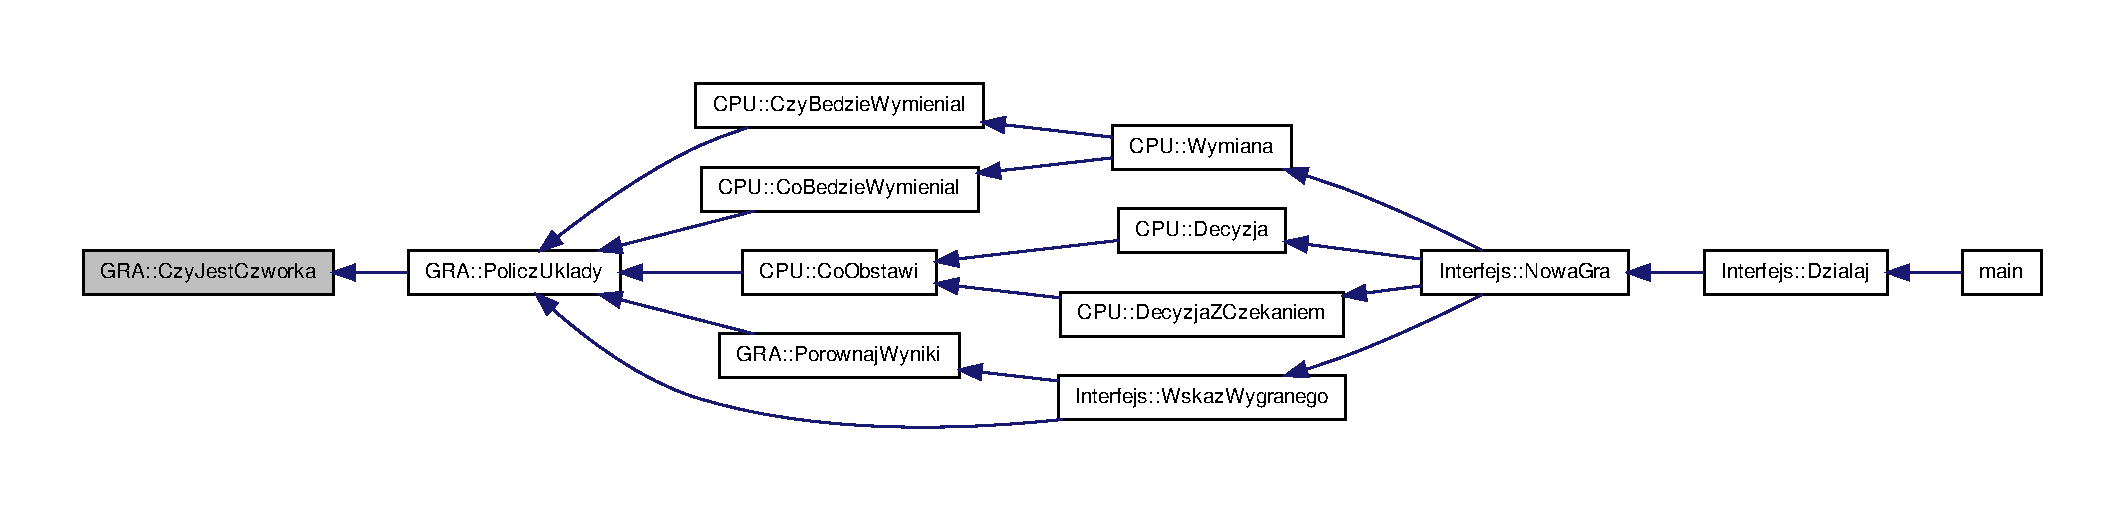
\includegraphics[width=350pt]{class_g_r_a_a1be2bb0326db17fde5861adb676224fb_icgraph}
\end{center}
\end{figure}


\hypertarget{class_g_r_a_a4d6b5d423f0f4761d04bbb59325417fd}{\index{G\-R\-A@{G\-R\-A}!Czy\-Jest\-Ful@{Czy\-Jest\-Ful}}
\index{Czy\-Jest\-Ful@{Czy\-Jest\-Ful}!GRA@{G\-R\-A}}
\subsubsection[{Czy\-Jest\-Ful}]{\setlength{\rightskip}{0pt plus 5cm}bool G\-R\-A\-::\-Czy\-Jest\-Ful (
\begin{DoxyParamCaption}
\item[{{\bf Gracz}}]{ziomek}
\end{DoxyParamCaption}
)}}\label{class_g_r_a_a4d6b5d423f0f4761d04bbb59325417fd}
\begin{DoxyReturn}{Zwraca}
Zwraca false lub true. 
\end{DoxyReturn}


Definicja w linii 609 pliku G\-R\-A.\-cpp.



Oto graf wywoływań tej funkcji\-:
\nopagebreak
\begin{figure}[H]
\begin{center}
\leavevmode
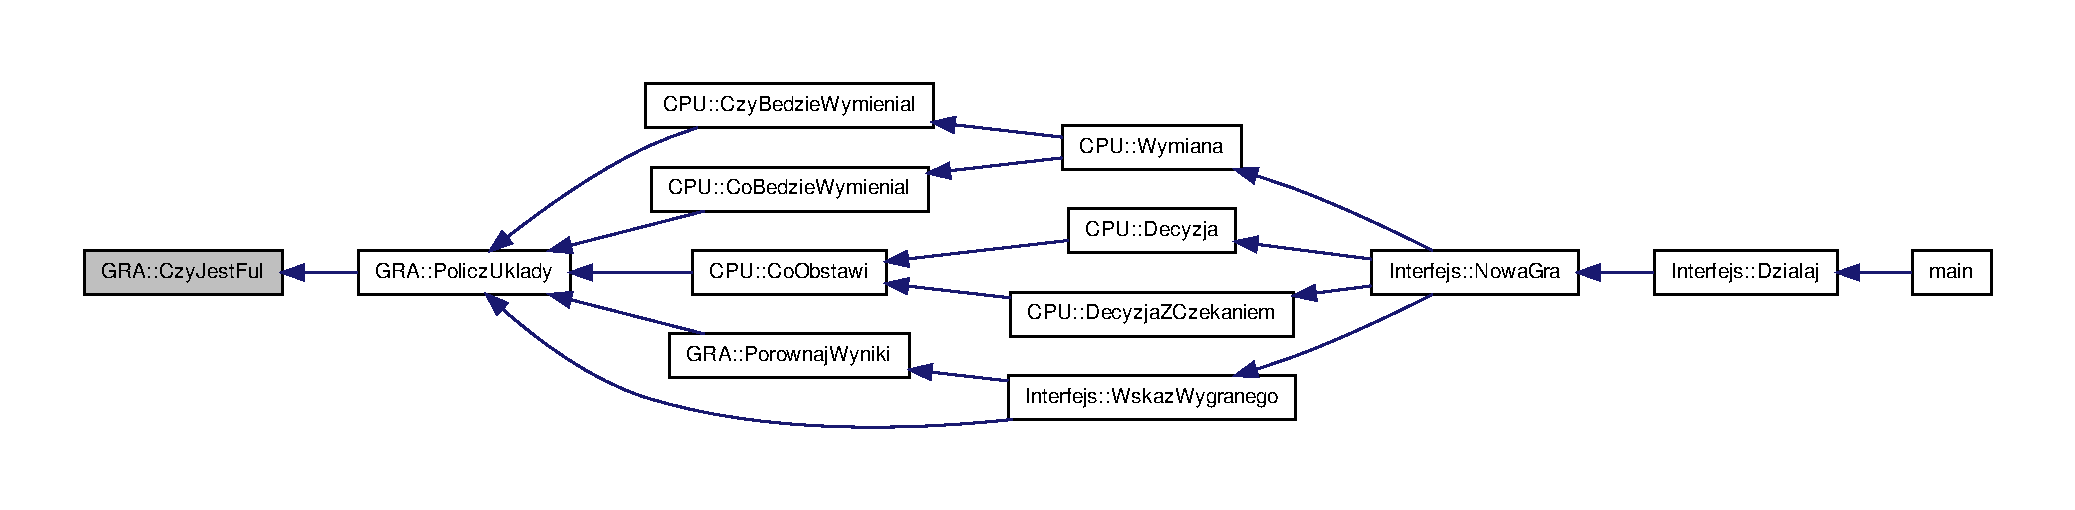
\includegraphics[width=350pt]{class_g_r_a_a4d6b5d423f0f4761d04bbb59325417fd_icgraph}
\end{center}
\end{figure}


\hypertarget{class_g_r_a_a04dd210d0146656fd70e2d10ccdf0065}{\index{G\-R\-A@{G\-R\-A}!Czy\-Jest\-Kolor@{Czy\-Jest\-Kolor}}
\index{Czy\-Jest\-Kolor@{Czy\-Jest\-Kolor}!GRA@{G\-R\-A}}
\subsubsection[{Czy\-Jest\-Kolor}]{\setlength{\rightskip}{0pt plus 5cm}bool G\-R\-A\-::\-Czy\-Jest\-Kolor (
\begin{DoxyParamCaption}
\item[{{\bf Gracz}}]{ziomek}
\end{DoxyParamCaption}
)}}\label{class_g_r_a_a04dd210d0146656fd70e2d10ccdf0065}
\begin{DoxyReturn}{Zwraca}
Zwraca false lub true. 
\end{DoxyReturn}


Definicja w linii 505 pliku G\-R\-A.\-cpp.



Oto graf wywoływań tej funkcji\-:
\nopagebreak
\begin{figure}[H]
\begin{center}
\leavevmode
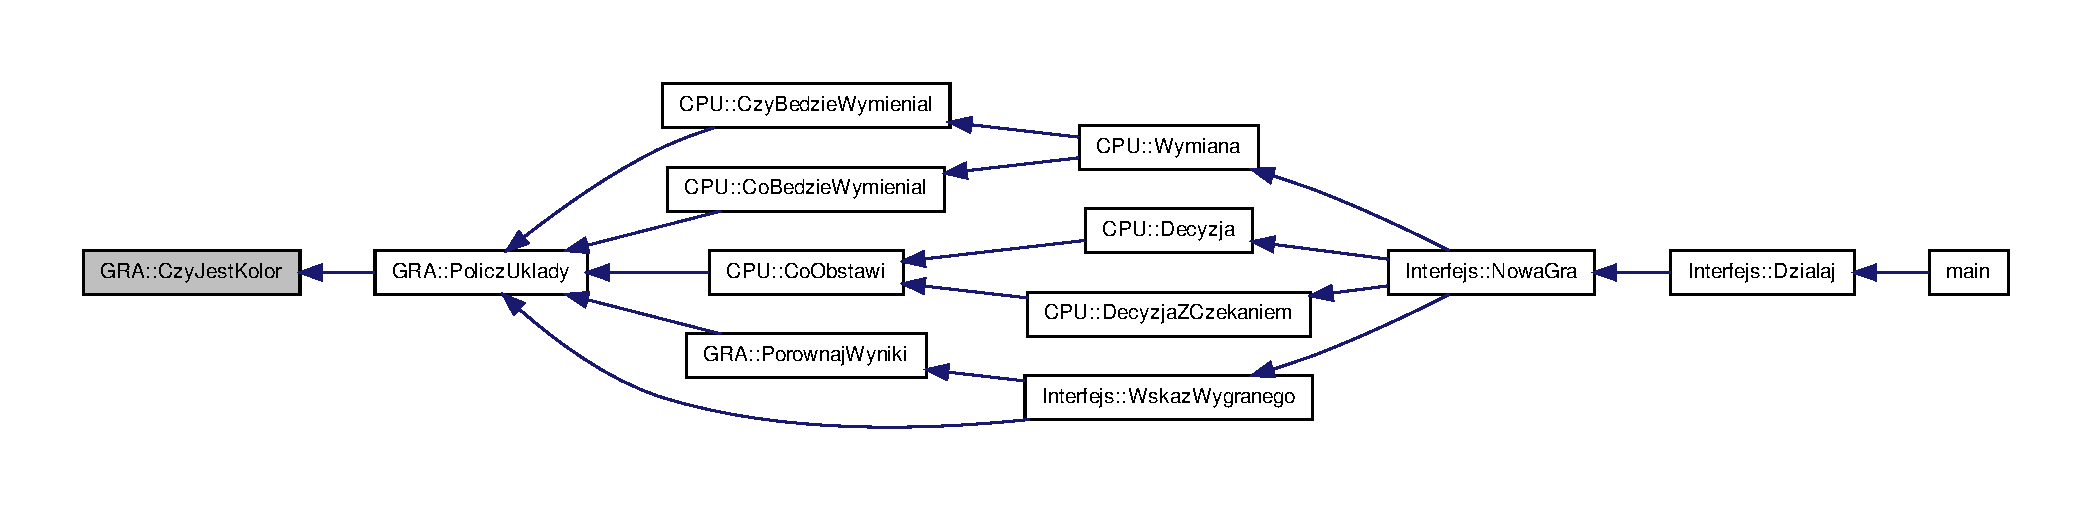
\includegraphics[width=350pt]{class_g_r_a_a04dd210d0146656fd70e2d10ccdf0065_icgraph}
\end{center}
\end{figure}


\hypertarget{class_g_r_a_a7c72639bade47c93f59e4d02344b29de}{\index{G\-R\-A@{G\-R\-A}!Czy\-Jest\-Para@{Czy\-Jest\-Para}}
\index{Czy\-Jest\-Para@{Czy\-Jest\-Para}!GRA@{G\-R\-A}}
\subsubsection[{Czy\-Jest\-Para}]{\setlength{\rightskip}{0pt plus 5cm}bool G\-R\-A\-::\-Czy\-Jest\-Para (
\begin{DoxyParamCaption}
\item[{{\bf Gracz}}]{ziomek}
\end{DoxyParamCaption}
)}}\label{class_g_r_a_a7c72639bade47c93f59e4d02344b29de}
\begin{DoxyReturn}{Zwraca}
Zwraca false lub true. 
\end{DoxyReturn}


Definicja w linii 298 pliku G\-R\-A.\-cpp.



Oto graf wywołań dla tej funkcji\-:\nopagebreak
\begin{figure}[H]
\begin{center}
\leavevmode
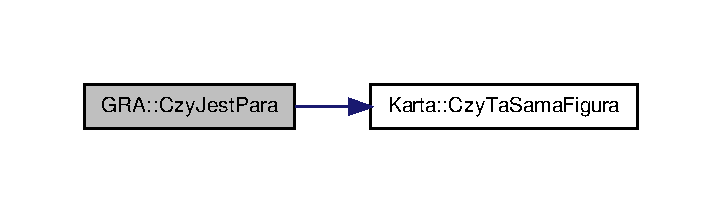
\includegraphics[width=346pt]{class_g_r_a_a7c72639bade47c93f59e4d02344b29de_cgraph}
\end{center}
\end{figure}




Oto graf wywoływań tej funkcji\-:
\nopagebreak
\begin{figure}[H]
\begin{center}
\leavevmode
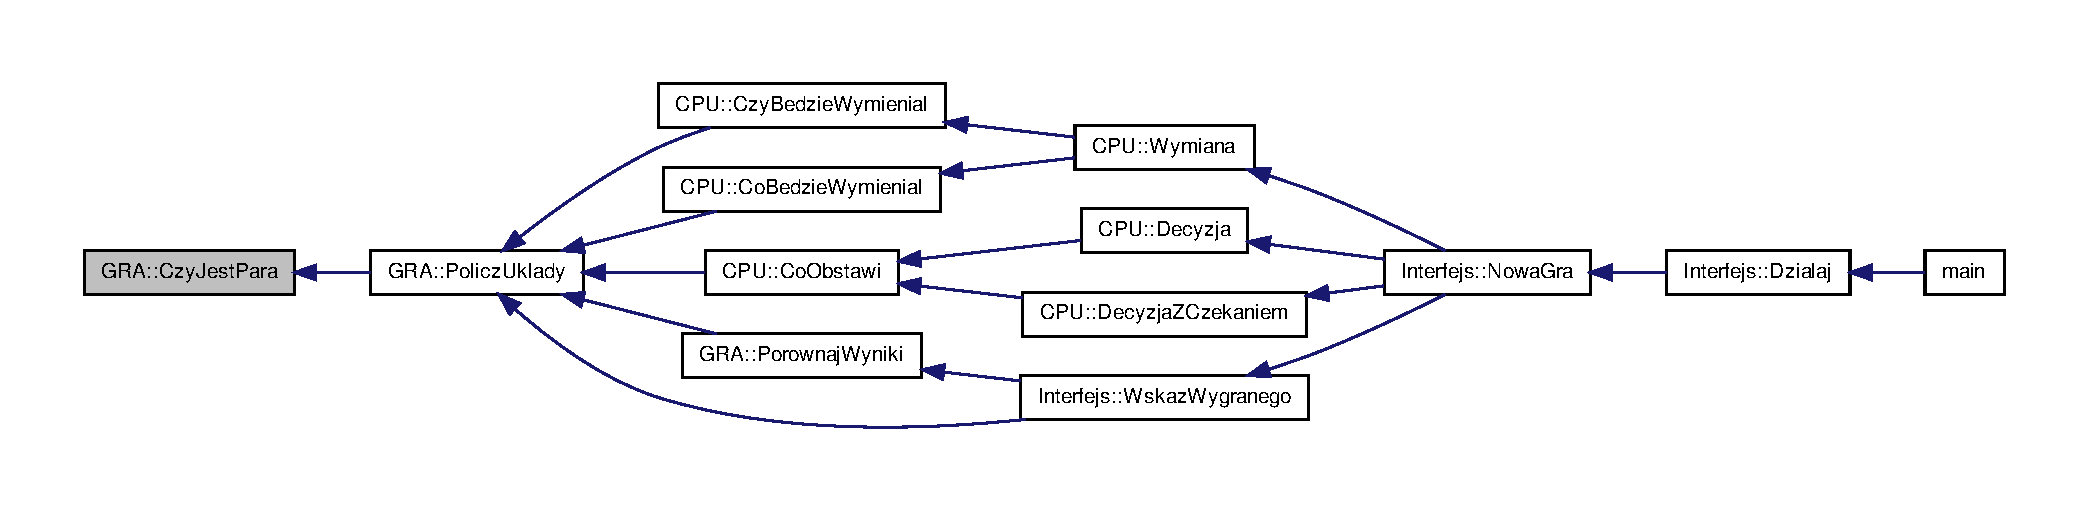
\includegraphics[width=350pt]{class_g_r_a_a7c72639bade47c93f59e4d02344b29de_icgraph}
\end{center}
\end{figure}


\hypertarget{class_g_r_a_a3fb6dbd37229ac58c84a0b4f5403a3d6}{\index{G\-R\-A@{G\-R\-A}!Czy\-Jest\-Strit@{Czy\-Jest\-Strit}}
\index{Czy\-Jest\-Strit@{Czy\-Jest\-Strit}!GRA@{G\-R\-A}}
\subsubsection[{Czy\-Jest\-Strit}]{\setlength{\rightskip}{0pt plus 5cm}bool G\-R\-A\-::\-Czy\-Jest\-Strit (
\begin{DoxyParamCaption}
\item[{{\bf Gracz}}]{ziomek}
\end{DoxyParamCaption}
)}}\label{class_g_r_a_a3fb6dbd37229ac58c84a0b4f5403a3d6}
\begin{DoxyReturn}{Zwraca}
Zwraca false lub true. 
\end{DoxyReturn}


Definicja w linii 462 pliku G\-R\-A.\-cpp.



Oto graf wywoływań tej funkcji\-:
\nopagebreak
\begin{figure}[H]
\begin{center}
\leavevmode
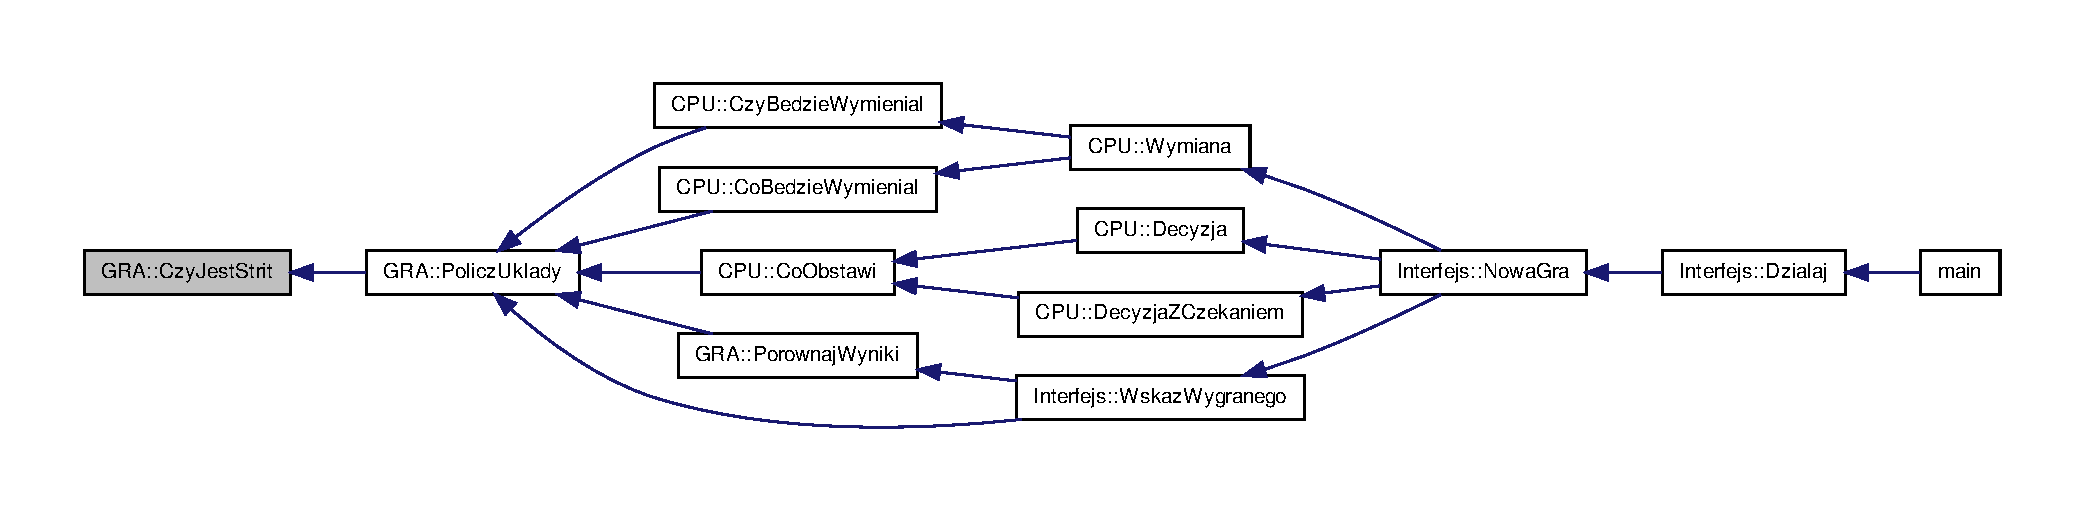
\includegraphics[width=350pt]{class_g_r_a_a3fb6dbd37229ac58c84a0b4f5403a3d6_icgraph}
\end{center}
\end{figure}


\hypertarget{class_g_r_a_ab62696649e029ba3adc5876dee3c8fbc}{\index{G\-R\-A@{G\-R\-A}!Czy\-Jest\-Trojka@{Czy\-Jest\-Trojka}}
\index{Czy\-Jest\-Trojka@{Czy\-Jest\-Trojka}!GRA@{G\-R\-A}}
\subsubsection[{Czy\-Jest\-Trojka}]{\setlength{\rightskip}{0pt plus 5cm}bool G\-R\-A\-::\-Czy\-Jest\-Trojka (
\begin{DoxyParamCaption}
\item[{{\bf Gracz}}]{ziomek}
\end{DoxyParamCaption}
)}}\label{class_g_r_a_ab62696649e029ba3adc5876dee3c8fbc}
\begin{DoxyReturn}{Zwraca}
Zwraca false lub true. 
\end{DoxyReturn}


Definicja w linii 366 pliku G\-R\-A.\-cpp.



Oto graf wywoływań tej funkcji\-:
\nopagebreak
\begin{figure}[H]
\begin{center}
\leavevmode
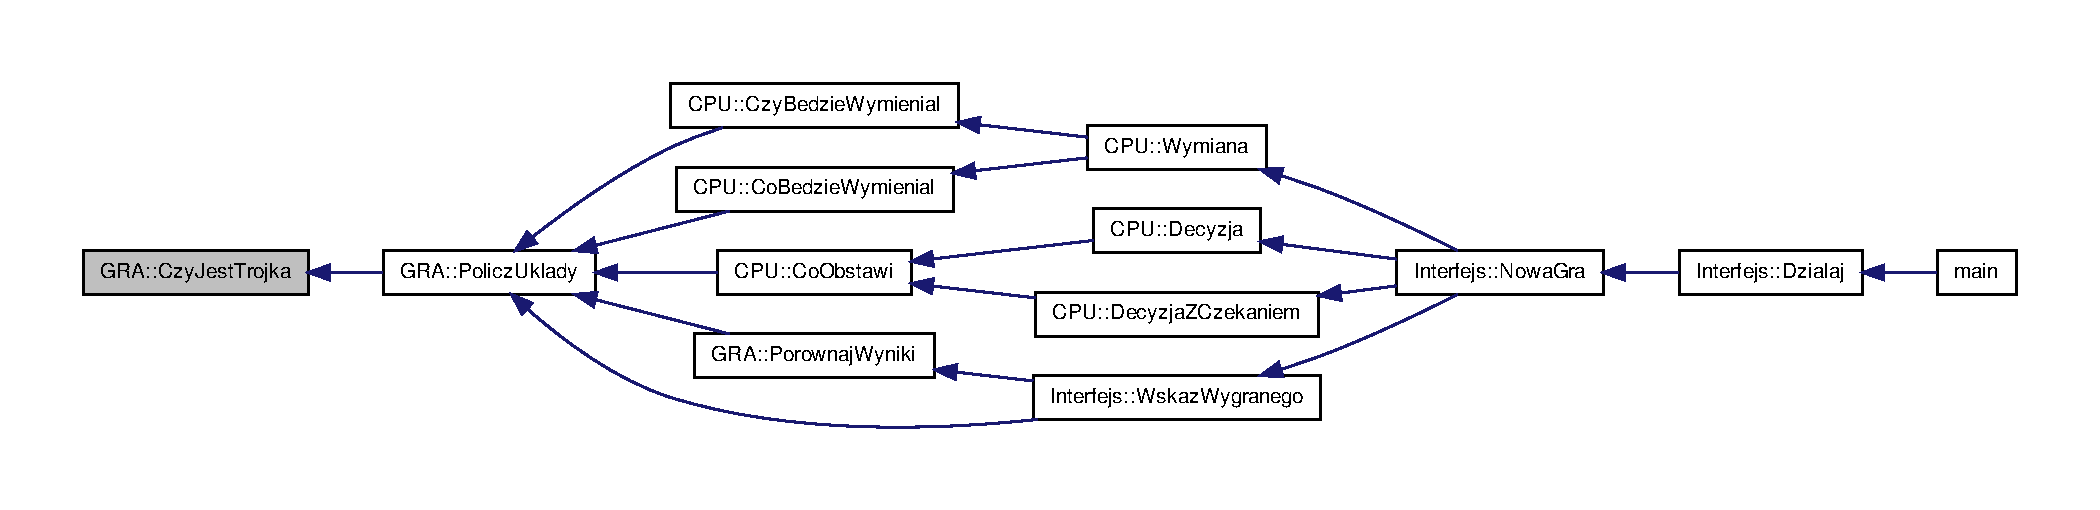
\includegraphics[width=350pt]{class_g_r_a_ab62696649e029ba3adc5876dee3c8fbc_icgraph}
\end{center}
\end{figure}


\hypertarget{class_g_r_a_a83ff1a2e629b7368180f5ac0cc06fcfd}{\index{G\-R\-A@{G\-R\-A}!Czy\-Sa\-Dwie\-Pary@{Czy\-Sa\-Dwie\-Pary}}
\index{Czy\-Sa\-Dwie\-Pary@{Czy\-Sa\-Dwie\-Pary}!GRA@{G\-R\-A}}
\subsubsection[{Czy\-Sa\-Dwie\-Pary}]{\setlength{\rightskip}{0pt plus 5cm}bool G\-R\-A\-::\-Czy\-Sa\-Dwie\-Pary (
\begin{DoxyParamCaption}
\item[{{\bf Gracz}}]{ziomek}
\end{DoxyParamCaption}
)}}\label{class_g_r_a_a83ff1a2e629b7368180f5ac0cc06fcfd}
\begin{DoxyReturn}{Zwraca}
Zwraca false lub true. 
\end{DoxyReturn}


Definicja w linii 316 pliku G\-R\-A.\-cpp.



Oto graf wywoływań tej funkcji\-:
\nopagebreak
\begin{figure}[H]
\begin{center}
\leavevmode
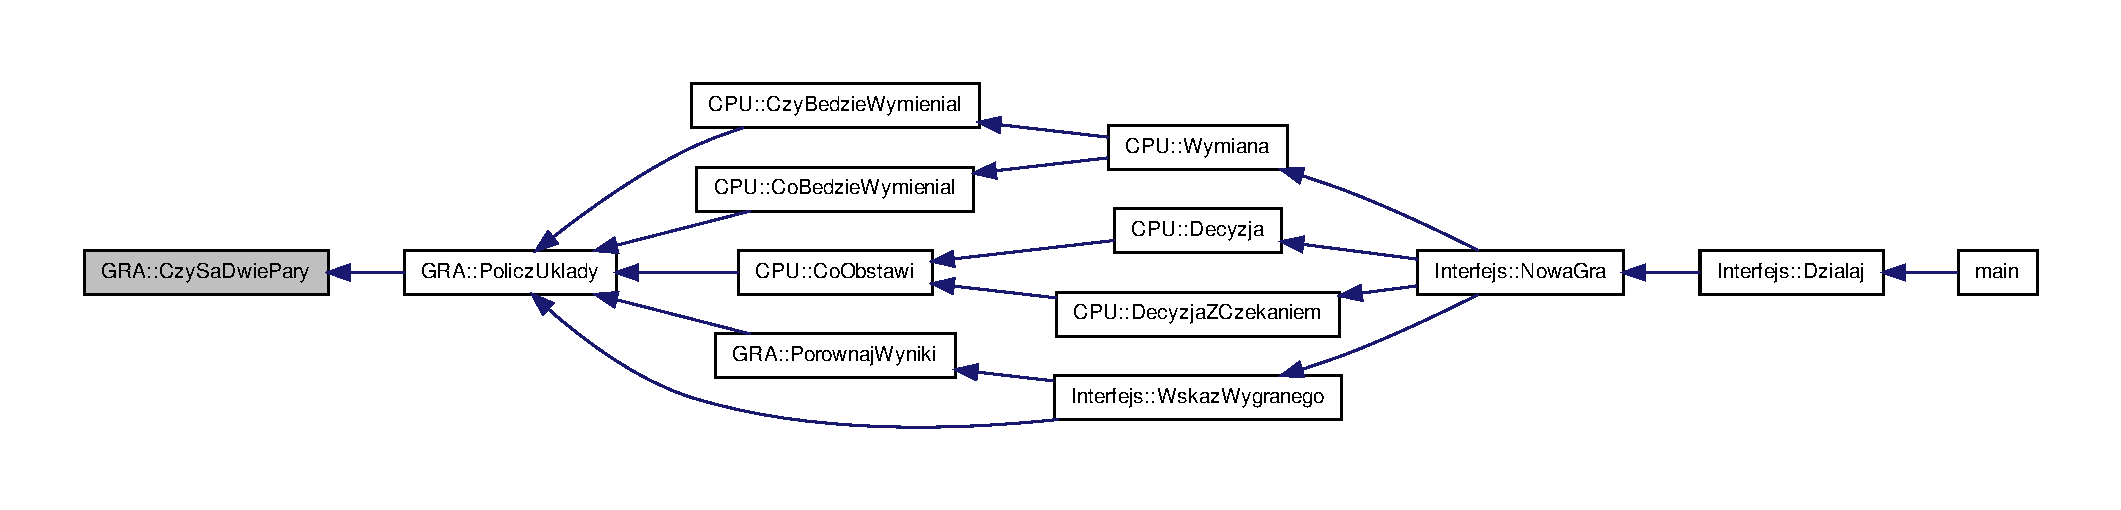
\includegraphics[width=350pt]{class_g_r_a_a83ff1a2e629b7368180f5ac0cc06fcfd_icgraph}
\end{center}
\end{figure}


\hypertarget{class_g_r_a_a08adc6b506a6fc09f75e0cfbe37a383a}{\index{G\-R\-A@{G\-R\-A}!Decyzja@{Decyzja}}
\index{Decyzja@{Decyzja}!GRA@{G\-R\-A}}
\subsubsection[{Decyzja}]{\setlength{\rightskip}{0pt plus 5cm}void G\-R\-A\-::\-Decyzja (
\begin{DoxyParamCaption}
\item[{{\bf Gracz} \&}]{ziomek}
\end{DoxyParamCaption}
)}}\label{class_g_r_a_a08adc6b506a6fc09f75e0cfbe37a383a}


Definicja w linii 1084 pliku G\-R\-A.\-cpp.



Oto graf wywoływań tej funkcji\-:
\nopagebreak
\begin{figure}[H]
\begin{center}
\leavevmode
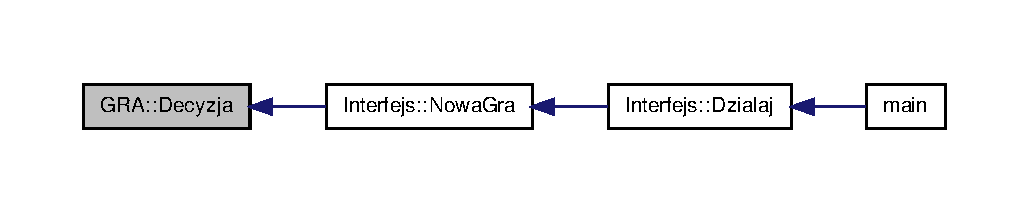
\includegraphics[width=350pt]{class_g_r_a_a08adc6b506a6fc09f75e0cfbe37a383a_icgraph}
\end{center}
\end{figure}


\hypertarget{class_g_r_a_af1183dcbde935bdf4f5ee1d6882b6d80}{\index{G\-R\-A@{G\-R\-A}!Decyzja\-Z\-Czekaniem@{Decyzja\-Z\-Czekaniem}}
\index{Decyzja\-Z\-Czekaniem@{Decyzja\-Z\-Czekaniem}!GRA@{G\-R\-A}}
\subsubsection[{Decyzja\-Z\-Czekaniem}]{\setlength{\rightskip}{0pt plus 5cm}void G\-R\-A\-::\-Decyzja\-Z\-Czekaniem (
\begin{DoxyParamCaption}
\item[{{\bf Gracz} \&}]{ziomek}
\end{DoxyParamCaption}
)}}\label{class_g_r_a_af1183dcbde935bdf4f5ee1d6882b6d80}


Definicja w linii 1171 pliku G\-R\-A.\-cpp.



Oto graf wywoływań tej funkcji\-:
\nopagebreak
\begin{figure}[H]
\begin{center}
\leavevmode
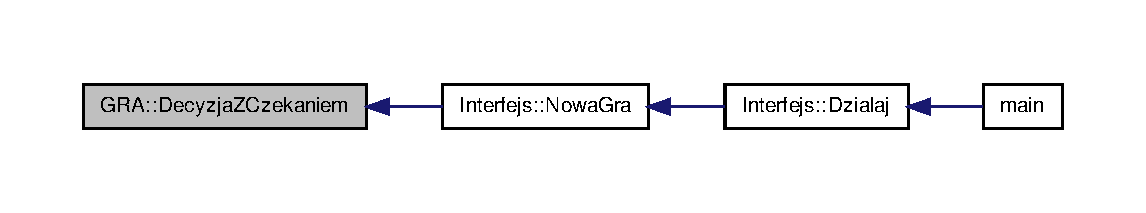
\includegraphics[width=350pt]{class_g_r_a_af1183dcbde935bdf4f5ee1d6882b6d80_icgraph}
\end{center}
\end{figure}


\hypertarget{class_g_r_a_abfc9b5fdad9fef80496cb5b6ece66ed9}{\index{G\-R\-A@{G\-R\-A}!Policz\-Uklady@{Policz\-Uklady}}
\index{Policz\-Uklady@{Policz\-Uklady}!GRA@{G\-R\-A}}
\subsubsection[{Policz\-Uklady}]{\setlength{\rightskip}{0pt plus 5cm}void G\-R\-A\-::\-Policz\-Uklady (
\begin{DoxyParamCaption}
\item[{{\bf Gracz} \&}]{ziomek}
\end{DoxyParamCaption}
)}}\label{class_g_r_a_abfc9b5fdad9fef80496cb5b6ece66ed9}


Definicja w linii 255 pliku G\-R\-A.\-cpp.



Oto graf wywołań dla tej funkcji\-:\nopagebreak
\begin{figure}[H]
\begin{center}
\leavevmode
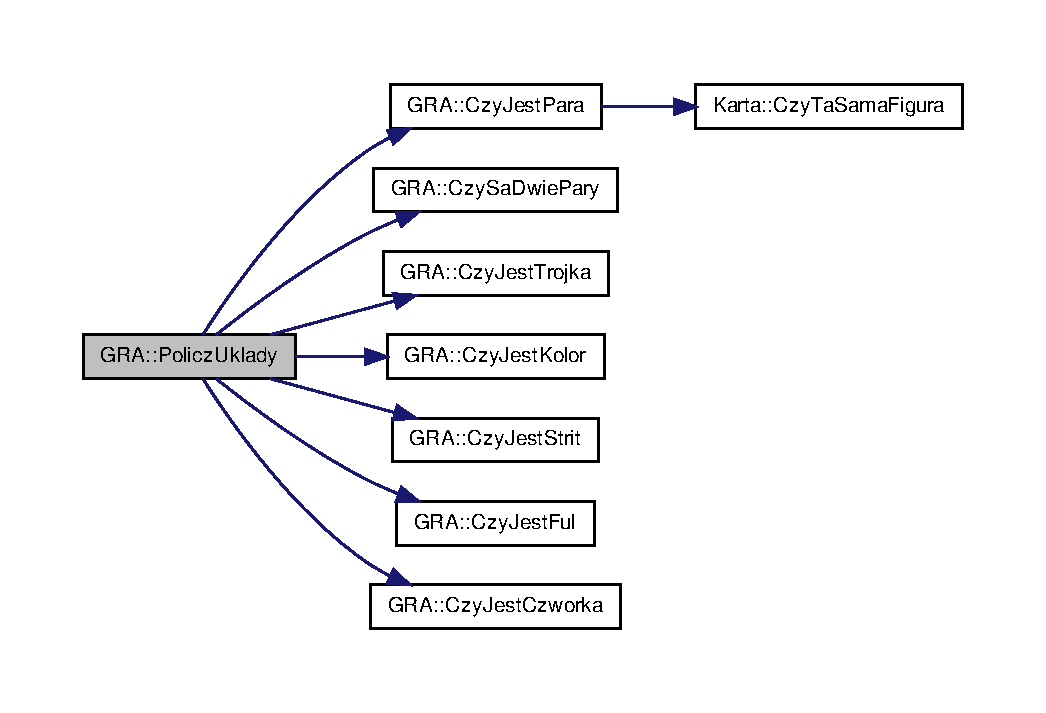
\includegraphics[width=350pt]{class_g_r_a_abfc9b5fdad9fef80496cb5b6ece66ed9_cgraph}
\end{center}
\end{figure}




Oto graf wywoływań tej funkcji\-:
\nopagebreak
\begin{figure}[H]
\begin{center}
\leavevmode
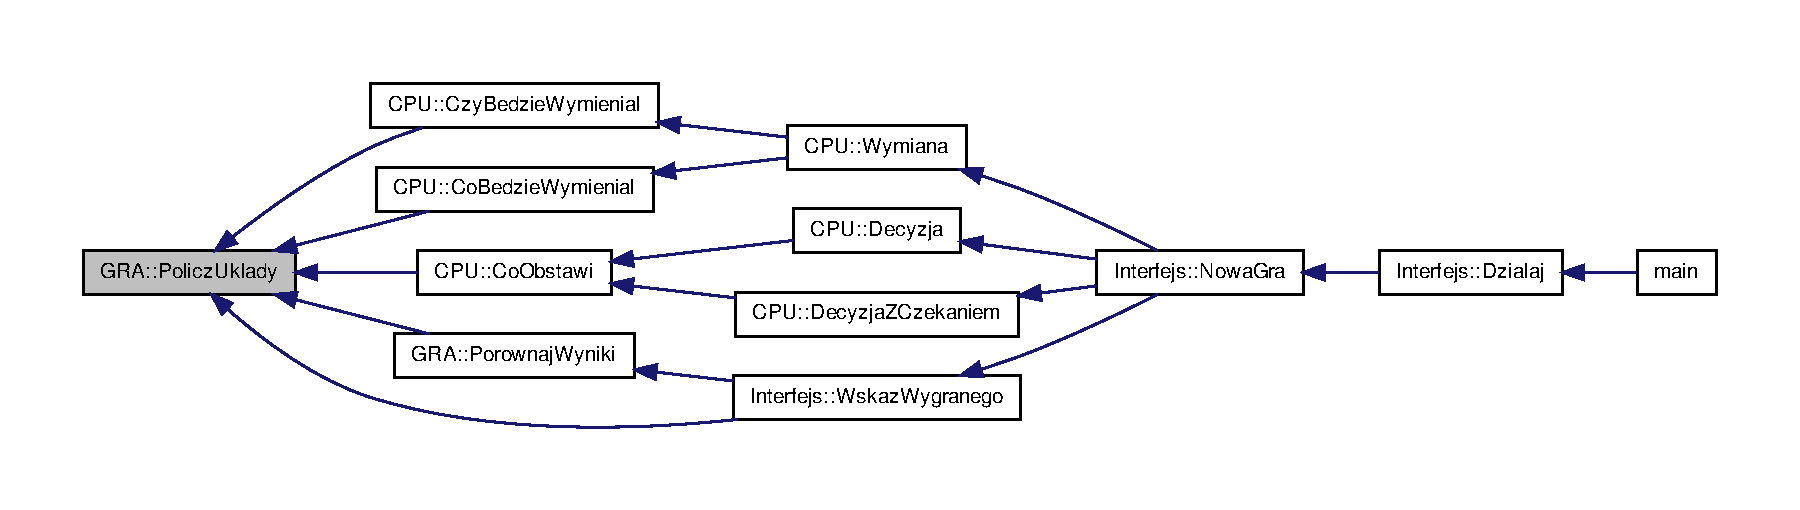
\includegraphics[width=350pt]{class_g_r_a_abfc9b5fdad9fef80496cb5b6ece66ed9_icgraph}
\end{center}
\end{figure}


\hypertarget{class_g_r_a_a0c6db7542b551b1c514f70b3ea9a358c}{\index{G\-R\-A@{G\-R\-A}!Porownaj\-Wyniki@{Porownaj\-Wyniki}}
\index{Porownaj\-Wyniki@{Porownaj\-Wyniki}!GRA@{G\-R\-A}}
\subsubsection[{Porownaj\-Wyniki}]{\setlength{\rightskip}{0pt plus 5cm}void G\-R\-A\-::\-Porownaj\-Wyniki (
\begin{DoxyParamCaption}
\item[{{\bf Gracz} \&}]{ziomek1, }
\item[{{\bf Gracz} \&}]{ziomek2}
\end{DoxyParamCaption}
)}}\label{class_g_r_a_a0c6db7542b551b1c514f70b3ea9a358c}


Definicja w linii 972 pliku G\-R\-A.\-cpp.



Oto graf wywołań dla tej funkcji\-:\nopagebreak
\begin{figure}[H]
\begin{center}
\leavevmode
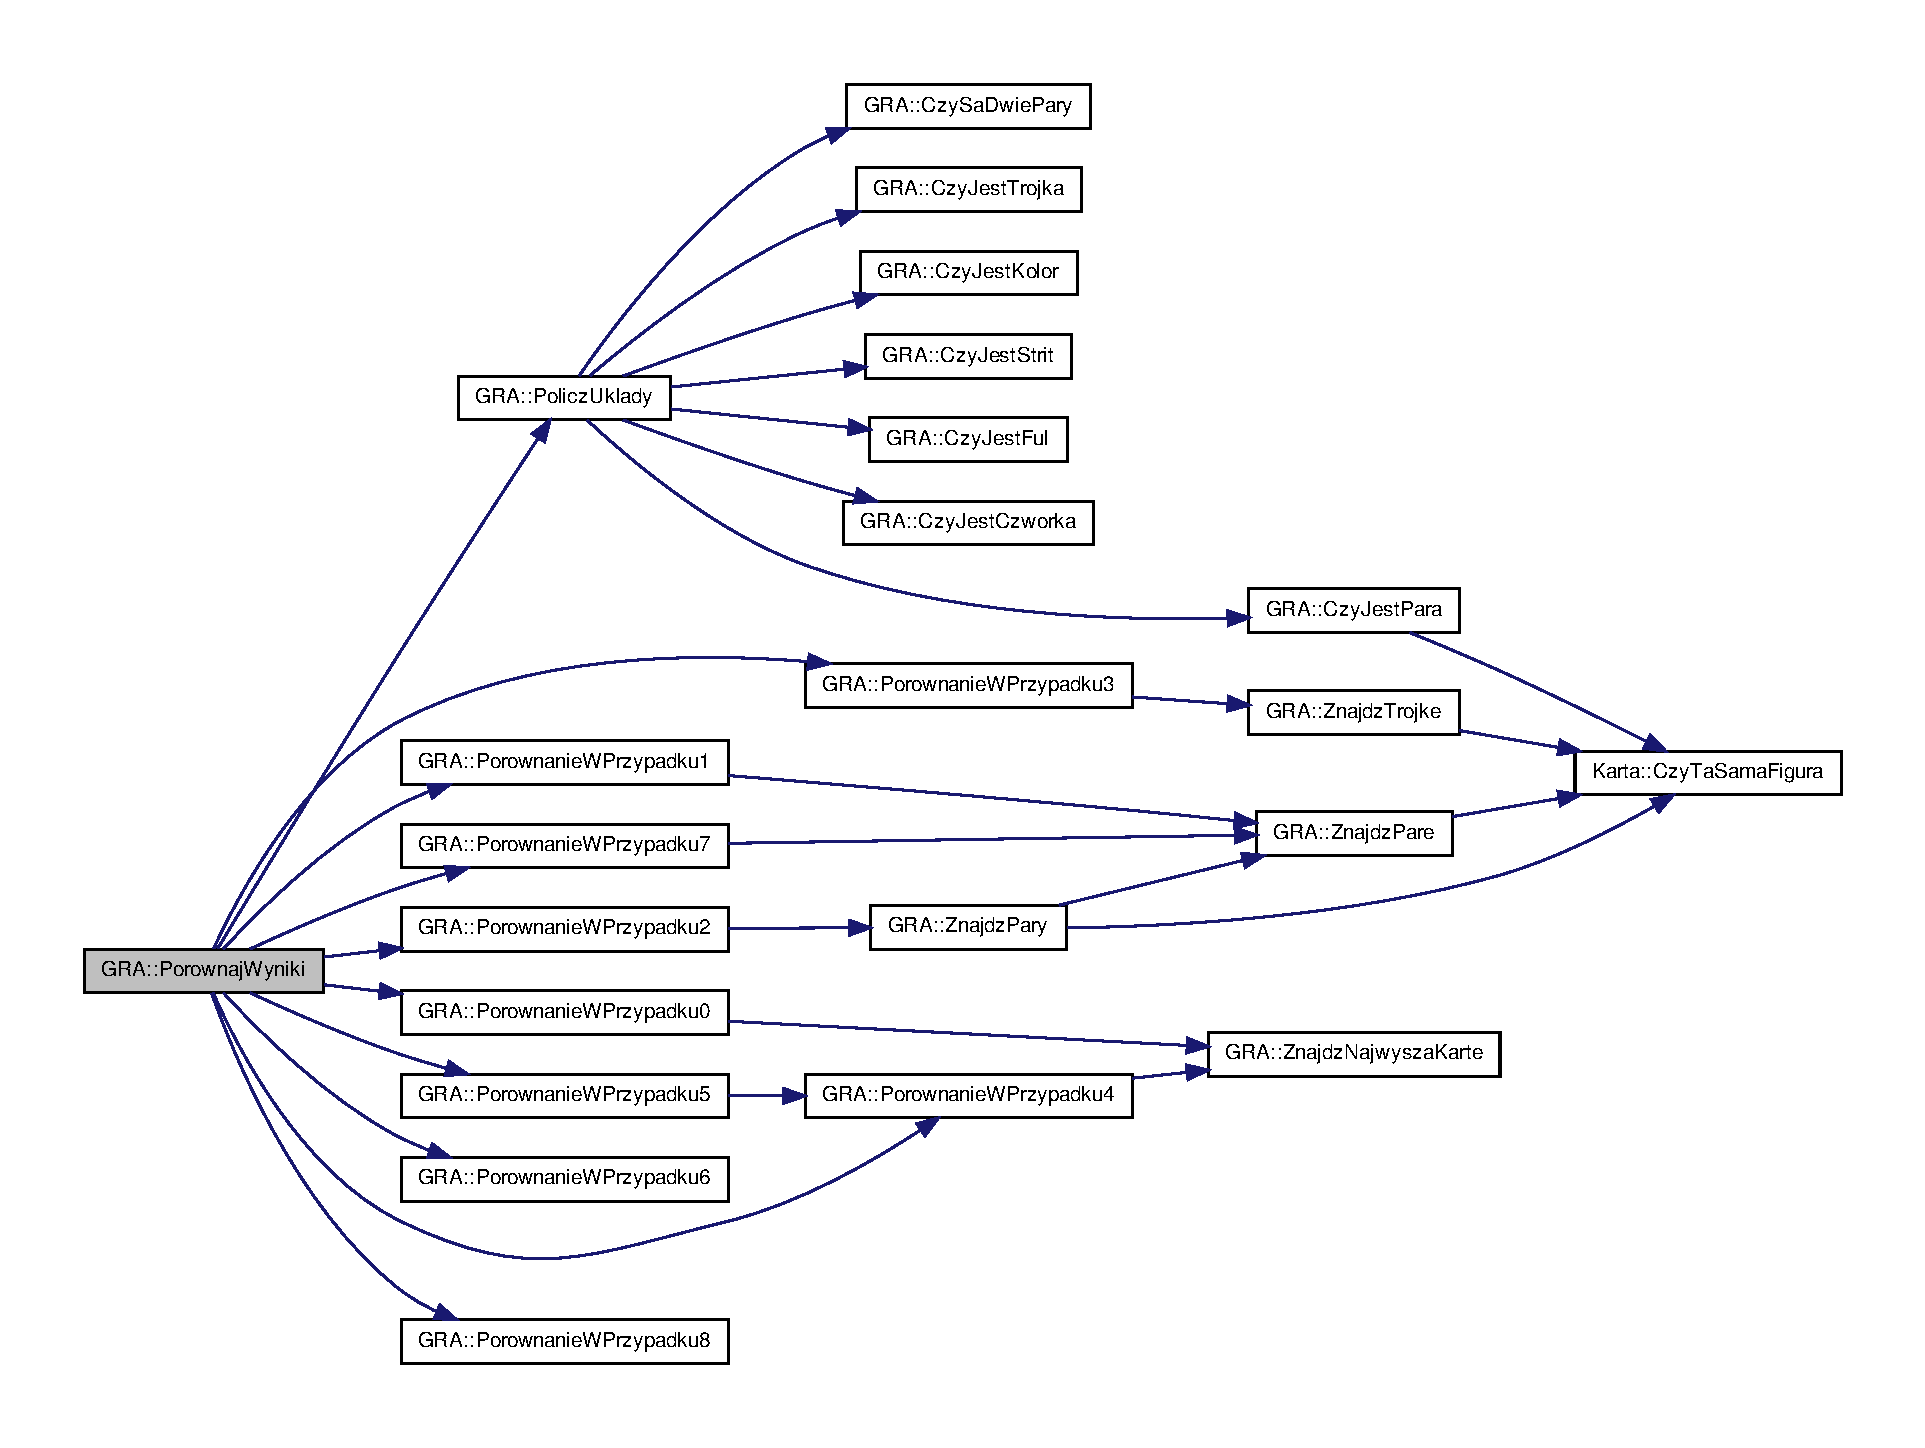
\includegraphics[width=350pt]{class_g_r_a_a0c6db7542b551b1c514f70b3ea9a358c_cgraph}
\end{center}
\end{figure}




Oto graf wywoływań tej funkcji\-:
\nopagebreak
\begin{figure}[H]
\begin{center}
\leavevmode
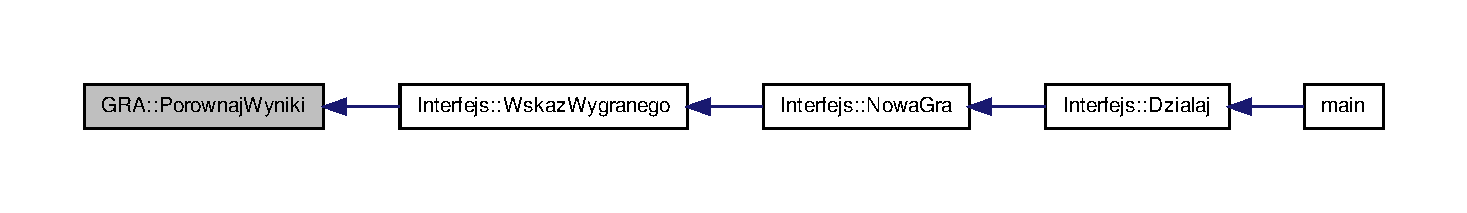
\includegraphics[width=350pt]{class_g_r_a_a0c6db7542b551b1c514f70b3ea9a358c_icgraph}
\end{center}
\end{figure}


\hypertarget{class_g_r_a_a2b8440a2cf458585286161fd46ad1bea}{\index{G\-R\-A@{G\-R\-A}!Porownanie\-W\-Przypadku0@{Porownanie\-W\-Przypadku0}}
\index{Porownanie\-W\-Przypadku0@{Porownanie\-W\-Przypadku0}!GRA@{G\-R\-A}}
\subsubsection[{Porownanie\-W\-Przypadku0}]{\setlength{\rightskip}{0pt plus 5cm}void G\-R\-A\-::\-Porownanie\-W\-Przypadku0 (
\begin{DoxyParamCaption}
\item[{{\bf Gracz} \&}]{ziomek1, }
\item[{{\bf Gracz} \&}]{ziomek2}
\end{DoxyParamCaption}
)\hspace{0.3cm}{\ttfamily [private]}}}\label{class_g_r_a_a2b8440a2cf458585286161fd46ad1bea}


Definicja w linii 677 pliku G\-R\-A.\-cpp.



Oto graf wywołań dla tej funkcji\-:\nopagebreak
\begin{figure}[H]
\begin{center}
\leavevmode
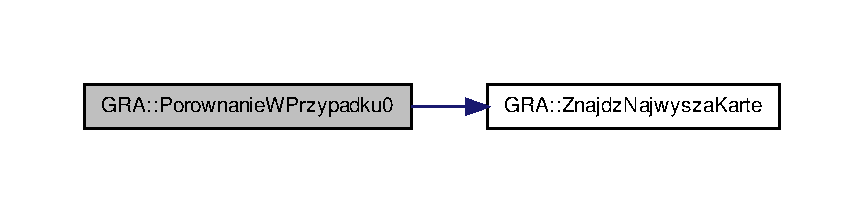
\includegraphics[width=350pt]{class_g_r_a_a2b8440a2cf458585286161fd46ad1bea_cgraph}
\end{center}
\end{figure}




Oto graf wywoływań tej funkcji\-:
\nopagebreak
\begin{figure}[H]
\begin{center}
\leavevmode
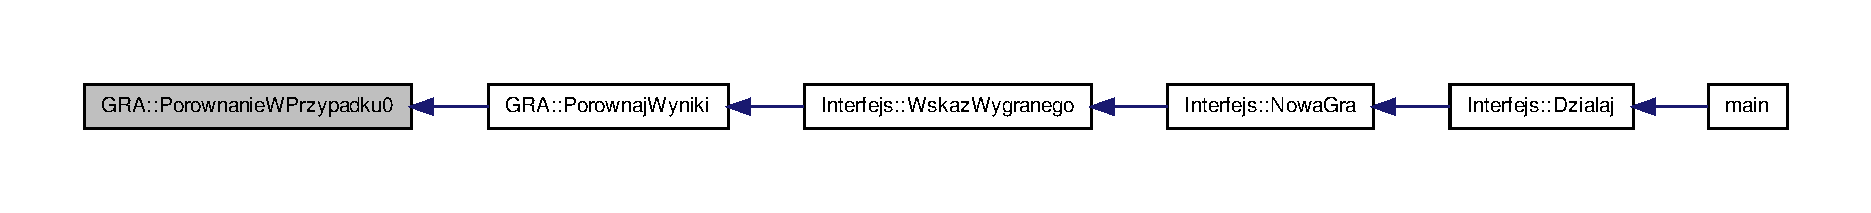
\includegraphics[width=350pt]{class_g_r_a_a2b8440a2cf458585286161fd46ad1bea_icgraph}
\end{center}
\end{figure}


\hypertarget{class_g_r_a_afcde718df260d05688ef36c7cf51de58}{\index{G\-R\-A@{G\-R\-A}!Porownanie\-W\-Przypadku1@{Porownanie\-W\-Przypadku1}}
\index{Porownanie\-W\-Przypadku1@{Porownanie\-W\-Przypadku1}!GRA@{G\-R\-A}}
\subsubsection[{Porownanie\-W\-Przypadku1}]{\setlength{\rightskip}{0pt plus 5cm}void G\-R\-A\-::\-Porownanie\-W\-Przypadku1 (
\begin{DoxyParamCaption}
\item[{{\bf Gracz} \&}]{ziomek1, }
\item[{{\bf Gracz} \&}]{ziomek2}
\end{DoxyParamCaption}
)\hspace{0.3cm}{\ttfamily [private]}}}\label{class_g_r_a_afcde718df260d05688ef36c7cf51de58}


Definicja w linii 700 pliku G\-R\-A.\-cpp.



Oto graf wywołań dla tej funkcji\-:\nopagebreak
\begin{figure}[H]
\begin{center}
\leavevmode
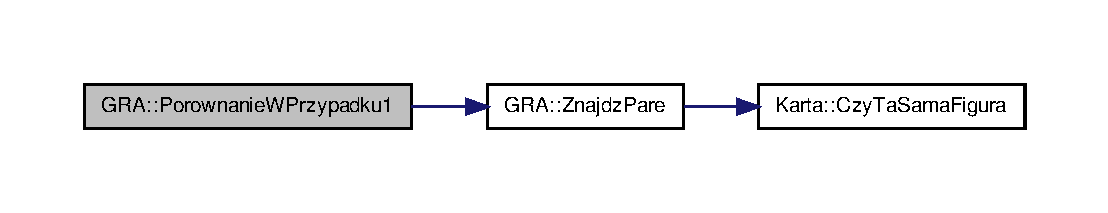
\includegraphics[width=350pt]{class_g_r_a_afcde718df260d05688ef36c7cf51de58_cgraph}
\end{center}
\end{figure}




Oto graf wywoływań tej funkcji\-:
\nopagebreak
\begin{figure}[H]
\begin{center}
\leavevmode
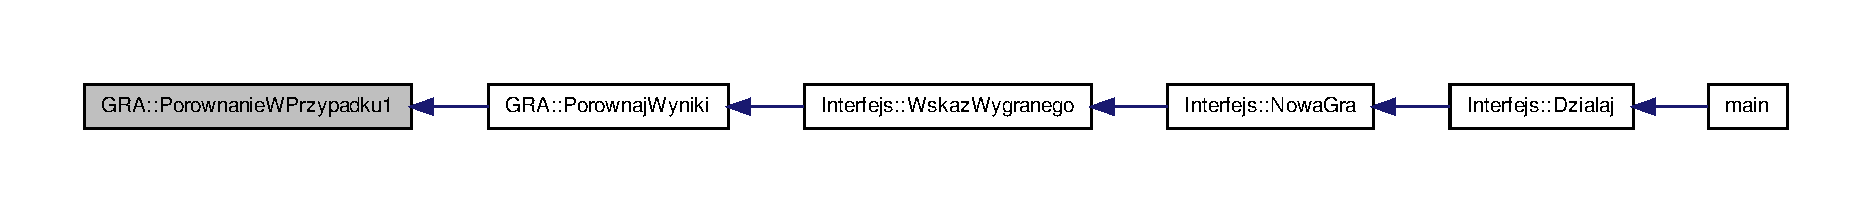
\includegraphics[width=350pt]{class_g_r_a_afcde718df260d05688ef36c7cf51de58_icgraph}
\end{center}
\end{figure}


\hypertarget{class_g_r_a_a51f60984eea162683d8e831952cceda8}{\index{G\-R\-A@{G\-R\-A}!Porownanie\-W\-Przypadku2@{Porownanie\-W\-Przypadku2}}
\index{Porownanie\-W\-Przypadku2@{Porownanie\-W\-Przypadku2}!GRA@{G\-R\-A}}
\subsubsection[{Porownanie\-W\-Przypadku2}]{\setlength{\rightskip}{0pt plus 5cm}void G\-R\-A\-::\-Porownanie\-W\-Przypadku2 (
\begin{DoxyParamCaption}
\item[{{\bf Gracz} \&}]{ziomek1, }
\item[{{\bf Gracz} \&}]{ziomek2}
\end{DoxyParamCaption}
)\hspace{0.3cm}{\ttfamily [private]}}}\label{class_g_r_a_a51f60984eea162683d8e831952cceda8}


Definicja w linii 723 pliku G\-R\-A.\-cpp.



Oto graf wywołań dla tej funkcji\-:\nopagebreak
\begin{figure}[H]
\begin{center}
\leavevmode
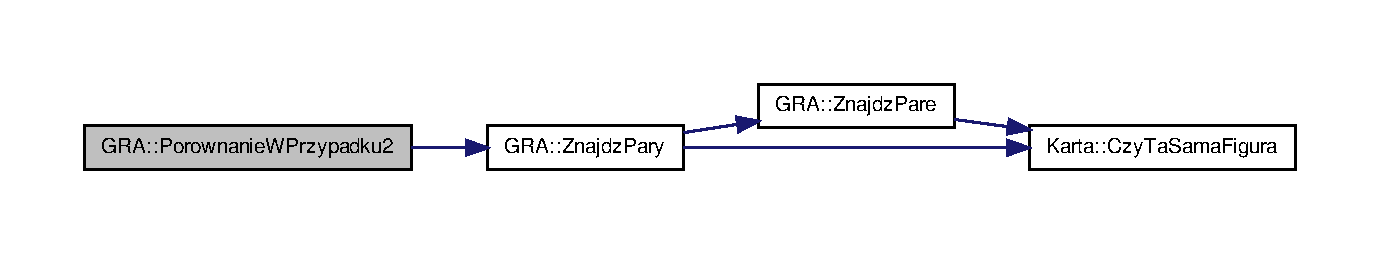
\includegraphics[width=350pt]{class_g_r_a_a51f60984eea162683d8e831952cceda8_cgraph}
\end{center}
\end{figure}




Oto graf wywoływań tej funkcji\-:
\nopagebreak
\begin{figure}[H]
\begin{center}
\leavevmode
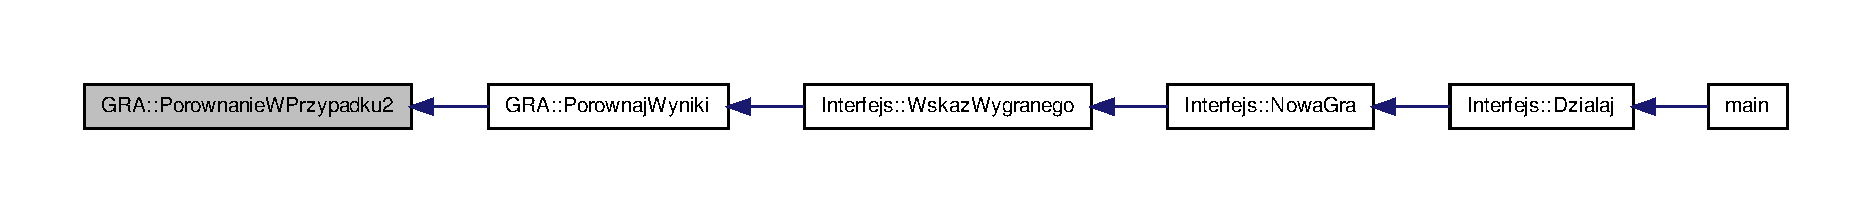
\includegraphics[width=350pt]{class_g_r_a_a51f60984eea162683d8e831952cceda8_icgraph}
\end{center}
\end{figure}


\hypertarget{class_g_r_a_a0f1a4cc74547c599d5b8b808e1613cd0}{\index{G\-R\-A@{G\-R\-A}!Porownanie\-W\-Przypadku3@{Porownanie\-W\-Przypadku3}}
\index{Porownanie\-W\-Przypadku3@{Porownanie\-W\-Przypadku3}!GRA@{G\-R\-A}}
\subsubsection[{Porownanie\-W\-Przypadku3}]{\setlength{\rightskip}{0pt plus 5cm}void G\-R\-A\-::\-Porownanie\-W\-Przypadku3 (
\begin{DoxyParamCaption}
\item[{{\bf Gracz} \&}]{ziomek1, }
\item[{{\bf Gracz} \&}]{ziomek2}
\end{DoxyParamCaption}
)\hspace{0.3cm}{\ttfamily [private]}}}\label{class_g_r_a_a0f1a4cc74547c599d5b8b808e1613cd0}


Definicja w linii 768 pliku G\-R\-A.\-cpp.



Oto graf wywołań dla tej funkcji\-:\nopagebreak
\begin{figure}[H]
\begin{center}
\leavevmode
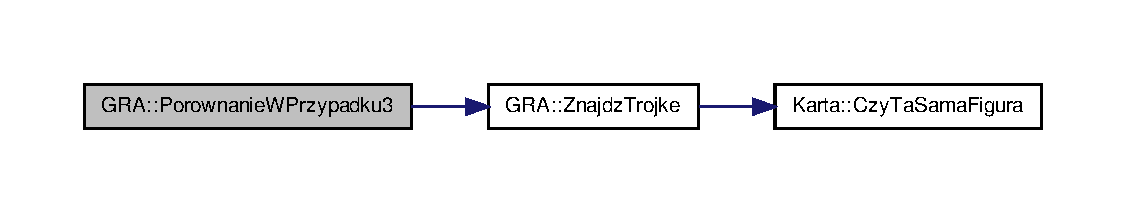
\includegraphics[width=350pt]{class_g_r_a_a0f1a4cc74547c599d5b8b808e1613cd0_cgraph}
\end{center}
\end{figure}




Oto graf wywoływań tej funkcji\-:
\nopagebreak
\begin{figure}[H]
\begin{center}
\leavevmode
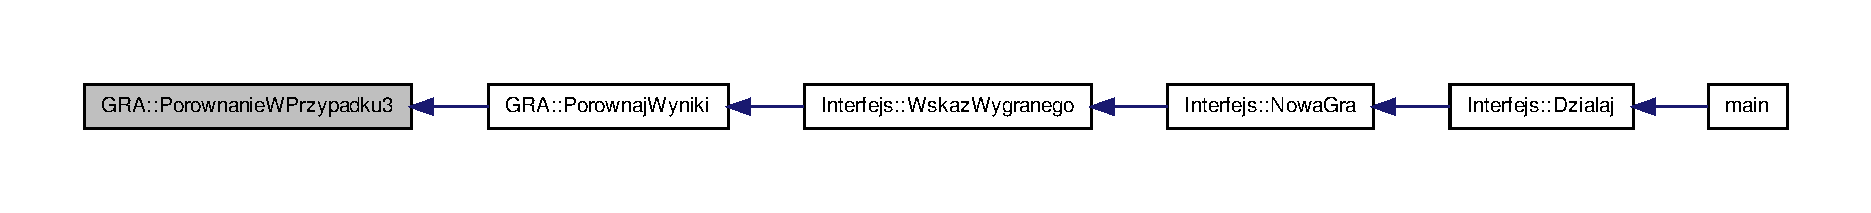
\includegraphics[width=350pt]{class_g_r_a_a0f1a4cc74547c599d5b8b808e1613cd0_icgraph}
\end{center}
\end{figure}


\hypertarget{class_g_r_a_a69bc4518f57fe02f9218fc6be253f687}{\index{G\-R\-A@{G\-R\-A}!Porownanie\-W\-Przypadku4@{Porownanie\-W\-Przypadku4}}
\index{Porownanie\-W\-Przypadku4@{Porownanie\-W\-Przypadku4}!GRA@{G\-R\-A}}
\subsubsection[{Porownanie\-W\-Przypadku4}]{\setlength{\rightskip}{0pt plus 5cm}void G\-R\-A\-::\-Porownanie\-W\-Przypadku4 (
\begin{DoxyParamCaption}
\item[{{\bf Gracz} \&}]{ziomek1, }
\item[{{\bf Gracz} \&}]{ziomek2}
\end{DoxyParamCaption}
)\hspace{0.3cm}{\ttfamily [private]}}}\label{class_g_r_a_a69bc4518f57fe02f9218fc6be253f687}


Definicja w linii 792 pliku G\-R\-A.\-cpp.



Oto graf wywołań dla tej funkcji\-:\nopagebreak
\begin{figure}[H]
\begin{center}
\leavevmode
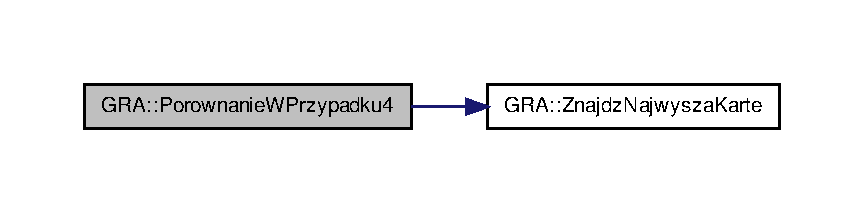
\includegraphics[width=350pt]{class_g_r_a_a69bc4518f57fe02f9218fc6be253f687_cgraph}
\end{center}
\end{figure}




Oto graf wywoływań tej funkcji\-:
\nopagebreak
\begin{figure}[H]
\begin{center}
\leavevmode
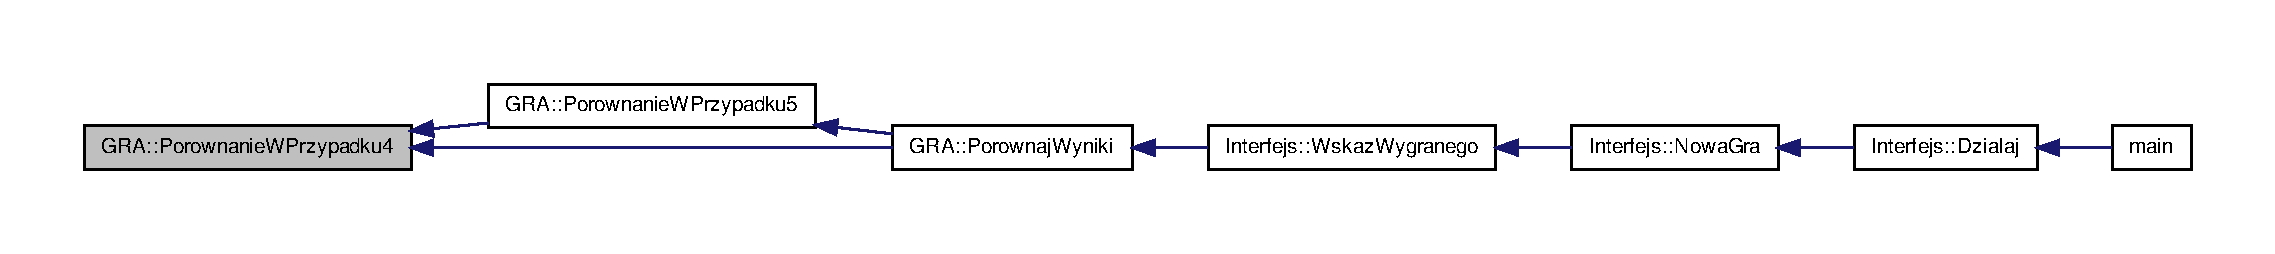
\includegraphics[width=350pt]{class_g_r_a_a69bc4518f57fe02f9218fc6be253f687_icgraph}
\end{center}
\end{figure}


\hypertarget{class_g_r_a_abd74a787e23a77dc6ccccece977ceef0}{\index{G\-R\-A@{G\-R\-A}!Porownanie\-W\-Przypadku5@{Porownanie\-W\-Przypadku5}}
\index{Porownanie\-W\-Przypadku5@{Porownanie\-W\-Przypadku5}!GRA@{G\-R\-A}}
\subsubsection[{Porownanie\-W\-Przypadku5}]{\setlength{\rightskip}{0pt plus 5cm}void G\-R\-A\-::\-Porownanie\-W\-Przypadku5 (
\begin{DoxyParamCaption}
\item[{{\bf Gracz} \&}]{ziomek1, }
\item[{{\bf Gracz} \&}]{ziomek2}
\end{DoxyParamCaption}
)\hspace{0.3cm}{\ttfamily [private]}}}\label{class_g_r_a_abd74a787e23a77dc6ccccece977ceef0}


Definicja w linii 815 pliku G\-R\-A.\-cpp.



Oto graf wywołań dla tej funkcji\-:\nopagebreak
\begin{figure}[H]
\begin{center}
\leavevmode
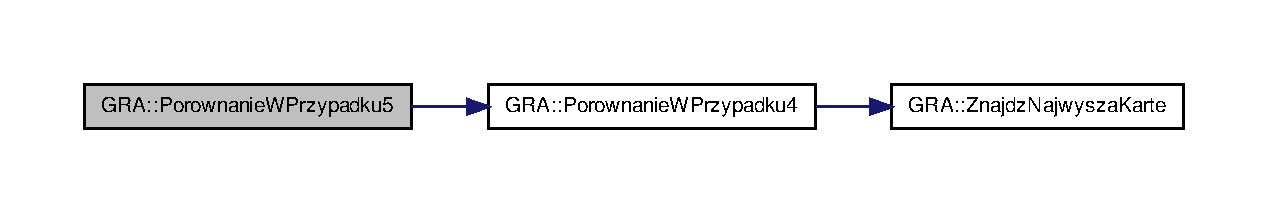
\includegraphics[width=350pt]{class_g_r_a_abd74a787e23a77dc6ccccece977ceef0_cgraph}
\end{center}
\end{figure}




Oto graf wywoływań tej funkcji\-:
\nopagebreak
\begin{figure}[H]
\begin{center}
\leavevmode
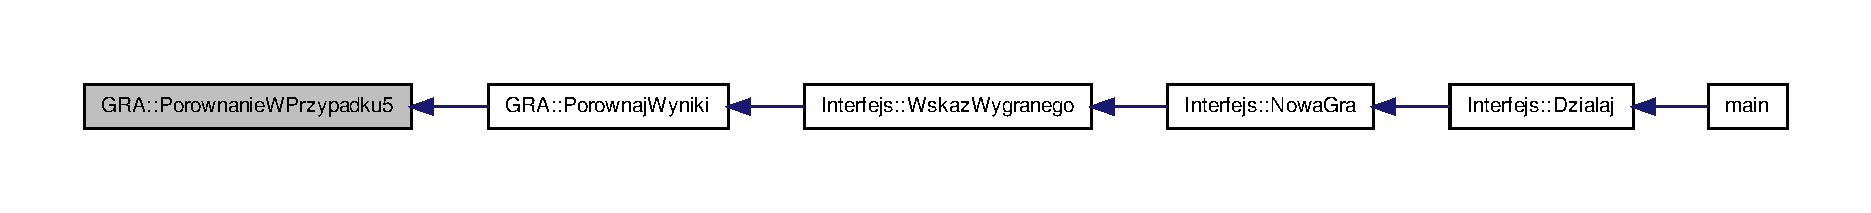
\includegraphics[width=350pt]{class_g_r_a_abd74a787e23a77dc6ccccece977ceef0_icgraph}
\end{center}
\end{figure}


\hypertarget{class_g_r_a_a58fe652c31046c129a81ec7d3f8755d0}{\index{G\-R\-A@{G\-R\-A}!Porownanie\-W\-Przypadku6@{Porownanie\-W\-Przypadku6}}
\index{Porownanie\-W\-Przypadku6@{Porownanie\-W\-Przypadku6}!GRA@{G\-R\-A}}
\subsubsection[{Porownanie\-W\-Przypadku6}]{\setlength{\rightskip}{0pt plus 5cm}void G\-R\-A\-::\-Porownanie\-W\-Przypadku6 (
\begin{DoxyParamCaption}
\item[{{\bf Gracz} \&}]{ziomek1, }
\item[{{\bf Gracz} \&}]{ziomek2}
\end{DoxyParamCaption}
)\hspace{0.3cm}{\ttfamily [private]}}}\label{class_g_r_a_a58fe652c31046c129a81ec7d3f8755d0}


Definicja w linii 820 pliku G\-R\-A.\-cpp.



Oto graf wywoływań tej funkcji\-:
\nopagebreak
\begin{figure}[H]
\begin{center}
\leavevmode
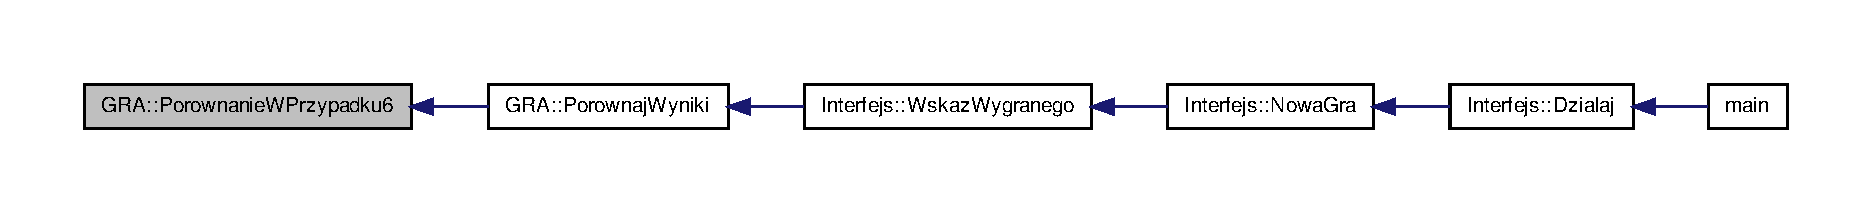
\includegraphics[width=350pt]{class_g_r_a_a58fe652c31046c129a81ec7d3f8755d0_icgraph}
\end{center}
\end{figure}


\hypertarget{class_g_r_a_a4a73ac7324002fe6f1d1c49cc447527e}{\index{G\-R\-A@{G\-R\-A}!Porownanie\-W\-Przypadku7@{Porownanie\-W\-Przypadku7}}
\index{Porownanie\-W\-Przypadku7@{Porownanie\-W\-Przypadku7}!GRA@{G\-R\-A}}
\subsubsection[{Porownanie\-W\-Przypadku7}]{\setlength{\rightskip}{0pt plus 5cm}void G\-R\-A\-::\-Porownanie\-W\-Przypadku7 (
\begin{DoxyParamCaption}
\item[{{\bf Gracz} \&}]{ziomek1, }
\item[{{\bf Gracz} \&}]{ziomek2}
\end{DoxyParamCaption}
)\hspace{0.3cm}{\ttfamily [private]}}}\label{class_g_r_a_a4a73ac7324002fe6f1d1c49cc447527e}


Definicja w linii 827 pliku G\-R\-A.\-cpp.



Oto graf wywołań dla tej funkcji\-:\nopagebreak
\begin{figure}[H]
\begin{center}
\leavevmode
\includegraphics[width=350pt]{class_g_r_a_a4a73ac7324002fe6f1d1c49cc447527e_cgraph}
\end{center}
\end{figure}




Oto graf wywoływań tej funkcji\-:
\nopagebreak
\begin{figure}[H]
\begin{center}
\leavevmode
\includegraphics[width=350pt]{class_g_r_a_a4a73ac7324002fe6f1d1c49cc447527e_icgraph}
\end{center}
\end{figure}


\hypertarget{class_g_r_a_a08ecbfc2389ce156e7e4cbb7a4bfbbcb}{\index{G\-R\-A@{G\-R\-A}!Porownanie\-W\-Przypadku8@{Porownanie\-W\-Przypadku8}}
\index{Porownanie\-W\-Przypadku8@{Porownanie\-W\-Przypadku8}!GRA@{G\-R\-A}}
\subsubsection[{Porownanie\-W\-Przypadku8}]{\setlength{\rightskip}{0pt plus 5cm}void G\-R\-A\-::\-Porownanie\-W\-Przypadku8 (
\begin{DoxyParamCaption}
\item[{{\bf Gracz} \&}]{ziomek1, }
\item[{{\bf Gracz} \&}]{ziomek2}
\end{DoxyParamCaption}
)\hspace{0.3cm}{\ttfamily [private]}}}\label{class_g_r_a_a08ecbfc2389ce156e7e4cbb7a4bfbbcb}


Definicja w linii 849 pliku G\-R\-A.\-cpp.



Oto graf wywoływań tej funkcji\-:
\nopagebreak
\begin{figure}[H]
\begin{center}
\leavevmode
\includegraphics[width=350pt]{class_g_r_a_a08ecbfc2389ce156e7e4cbb7a4bfbbcb_icgraph}
\end{center}
\end{figure}


\hypertarget{class_g_r_a_ab18509b806b22568ba97a8ab4f121ae2}{\index{G\-R\-A@{G\-R\-A}!Potasuj@{Potasuj}}
\index{Potasuj@{Potasuj}!GRA@{G\-R\-A}}
\subsubsection[{Potasuj}]{\setlength{\rightskip}{0pt plus 5cm}void G\-R\-A\-::\-Potasuj (
\begin{DoxyParamCaption}
{}
\end{DoxyParamCaption}
)}}\label{class_g_r_a_ab18509b806b22568ba97a8ab4f121ae2}


Definicja w linii 1073 pliku G\-R\-A.\-cpp.



Oto graf wywołań dla tej funkcji\-:\nopagebreak
\begin{figure}[H]
\begin{center}
\leavevmode
\includegraphics[width=272pt]{class_g_r_a_ab18509b806b22568ba97a8ab4f121ae2_cgraph}
\end{center}
\end{figure}




Oto graf wywoływań tej funkcji\-:
\nopagebreak
\begin{figure}[H]
\begin{center}
\leavevmode
\includegraphics[width=350pt]{class_g_r_a_ab18509b806b22568ba97a8ab4f121ae2_icgraph}
\end{center}
\end{figure}


\hypertarget{class_g_r_a_a3d86b57e35ee8ff610a056c92dfa325b}{\index{G\-R\-A@{G\-R\-A}!Rozdaj@{Rozdaj}}
\index{Rozdaj@{Rozdaj}!GRA@{G\-R\-A}}
\subsubsection[{Rozdaj}]{\setlength{\rightskip}{0pt plus 5cm}void G\-R\-A\-::\-Rozdaj (
\begin{DoxyParamCaption}
\item[{{\bf Gracz} \&}]{gosc}
\end{DoxyParamCaption}
)}}\label{class_g_r_a_a3d86b57e35ee8ff610a056c92dfa325b}


Definicja w linii 1055 pliku G\-R\-A.\-cpp.



Oto graf wywołań dla tej funkcji\-:\nopagebreak
\begin{figure}[H]
\begin{center}
\leavevmode
\includegraphics[width=292pt]{class_g_r_a_a3d86b57e35ee8ff610a056c92dfa325b_cgraph}
\end{center}
\end{figure}




Oto graf wywoływań tej funkcji\-:
\nopagebreak
\begin{figure}[H]
\begin{center}
\leavevmode
\includegraphics[width=350pt]{class_g_r_a_a3d86b57e35ee8ff610a056c92dfa325b_icgraph}
\end{center}
\end{figure}


\hypertarget{class_g_r_a_a28a2c64b762a24b489af437c7eef6040}{\index{G\-R\-A@{G\-R\-A}!Rozdaj\-Kase@{Rozdaj\-Kase}}
\index{Rozdaj\-Kase@{Rozdaj\-Kase}!GRA@{G\-R\-A}}
\subsubsection[{Rozdaj\-Kase}]{\setlength{\rightskip}{0pt plus 5cm}void G\-R\-A\-::\-Rozdaj\-Kase (
\begin{DoxyParamCaption}
\item[{{\bf Gracz} \&}]{ziomek, }
\item[{int}]{ile}
\end{DoxyParamCaption}
)}}\label{class_g_r_a_a28a2c64b762a24b489af437c7eef6040}


Definicja w linii 1079 pliku G\-R\-A.\-cpp.



Oto graf wywoływań tej funkcji\-:
\nopagebreak
\begin{figure}[H]
\begin{center}
\leavevmode
\includegraphics[width=350pt]{class_g_r_a_a28a2c64b762a24b489af437c7eef6040_icgraph}
\end{center}
\end{figure}


\hypertarget{class_g_r_a_a4ffb4d5d97261a8cd2220a6b59616bb6}{\index{G\-R\-A@{G\-R\-A}!Wymiana@{Wymiana}}
\index{Wymiana@{Wymiana}!GRA@{G\-R\-A}}
\subsubsection[{Wymiana}]{\setlength{\rightskip}{0pt plus 5cm}void G\-R\-A\-::\-Wymiana (
\begin{DoxyParamCaption}
\item[{{\bf Gracz} \&}]{ziomek}
\end{DoxyParamCaption}
)}}\label{class_g_r_a_a4ffb4d5d97261a8cd2220a6b59616bb6}


Definicja w linii 9 pliku G\-R\-A.\-cpp.



Oto graf wywołań dla tej funkcji\-:\nopagebreak
\begin{figure}[H]
\begin{center}
\leavevmode
\includegraphics[width=350pt]{class_g_r_a_a4ffb4d5d97261a8cd2220a6b59616bb6_cgraph}
\end{center}
\end{figure}




Oto graf wywoływań tej funkcji\-:
\nopagebreak
\begin{figure}[H]
\begin{center}
\leavevmode
\includegraphics[width=350pt]{class_g_r_a_a4ffb4d5d97261a8cd2220a6b59616bb6_icgraph}
\end{center}
\end{figure}


\hypertarget{class_g_r_a_a99c72e824c90f1bdbb34626e67d83c15}{\index{G\-R\-A@{G\-R\-A}!Wymien@{Wymien}}
\index{Wymien@{Wymien}!GRA@{G\-R\-A}}
\subsubsection[{Wymien}]{\setlength{\rightskip}{0pt plus 5cm}void G\-R\-A\-::\-Wymien (
\begin{DoxyParamCaption}
\item[{{\bf Karta} \&}]{Karteczka}
\end{DoxyParamCaption}
)}}\label{class_g_r_a_a99c72e824c90f1bdbb34626e67d83c15}


Definicja w linii 238 pliku G\-R\-A.\-cpp.



Oto graf wywołań dla tej funkcji\-:\nopagebreak
\begin{figure}[H]
\begin{center}
\leavevmode
\includegraphics[width=296pt]{class_g_r_a_a99c72e824c90f1bdbb34626e67d83c15_cgraph}
\end{center}
\end{figure}




Oto graf wywoływań tej funkcji\-:
\nopagebreak
\begin{figure}[H]
\begin{center}
\leavevmode
\includegraphics[width=350pt]{class_g_r_a_a99c72e824c90f1bdbb34626e67d83c15_icgraph}
\end{center}
\end{figure}


\hypertarget{class_g_r_a_a532269809ccd27cde2c8a7822bfc1a43}{\index{G\-R\-A@{G\-R\-A}!Wyswietl\-Instrukcje@{Wyswietl\-Instrukcje}}
\index{Wyswietl\-Instrukcje@{Wyswietl\-Instrukcje}!GRA@{G\-R\-A}}
\subsubsection[{Wyswietl\-Instrukcje}]{\setlength{\rightskip}{0pt plus 5cm}void G\-R\-A\-::\-Wyswietl\-Instrukcje (
\begin{DoxyParamCaption}
{}
\end{DoxyParamCaption}
)}}\label{class_g_r_a_a532269809ccd27cde2c8a7822bfc1a43}


Definicja w linii 246 pliku G\-R\-A.\-cpp.



Oto graf wywoływań tej funkcji\-:
\nopagebreak
\begin{figure}[H]
\begin{center}
\leavevmode
\includegraphics[width=350pt]{class_g_r_a_a532269809ccd27cde2c8a7822bfc1a43_icgraph}
\end{center}
\end{figure}


\hypertarget{class_g_r_a_aba14465002d4fa6440beca25bf3de2bc}{\index{G\-R\-A@{G\-R\-A}!Znajdz\-Najwysza\-Karte@{Znajdz\-Najwysza\-Karte}}
\index{Znajdz\-Najwysza\-Karte@{Znajdz\-Najwysza\-Karte}!GRA@{G\-R\-A}}
\subsubsection[{Znajdz\-Najwysza\-Karte}]{\setlength{\rightskip}{0pt plus 5cm}int G\-R\-A\-::\-Znajdz\-Najwysza\-Karte (
\begin{DoxyParamCaption}
\item[{{\bf Gracz}}]{ziomek}
\end{DoxyParamCaption}
)}}\label{class_g_r_a_aba14465002d4fa6440beca25bf3de2bc}
\begin{DoxyReturn}{Zwraca}
Zwraca figure ktora jest najwyzsza w kartach gracza. 
\end{DoxyReturn}


Definicja w linii 859 pliku G\-R\-A.\-cpp.



Oto graf wywoływań tej funkcji\-:
\nopagebreak
\begin{figure}[H]
\begin{center}
\leavevmode
\includegraphics[width=350pt]{class_g_r_a_aba14465002d4fa6440beca25bf3de2bc_icgraph}
\end{center}
\end{figure}


\hypertarget{class_g_r_a_a2f160ac8a217e52308423ddc950488d5}{\index{G\-R\-A@{G\-R\-A}!Znajdz\-Pare@{Znajdz\-Pare}}
\index{Znajdz\-Pare@{Znajdz\-Pare}!GRA@{G\-R\-A}}
\subsubsection[{Znajdz\-Pare}]{\setlength{\rightskip}{0pt plus 5cm}int G\-R\-A\-::\-Znajdz\-Pare (
\begin{DoxyParamCaption}
\item[{{\bf Gracz}}]{ziomek}
\end{DoxyParamCaption}
)}}\label{class_g_r_a_a2f160ac8a217e52308423ddc950488d5}
\begin{DoxyReturn}{Zwraca}
Zwraca figure ktora jest w parze. 
\end{DoxyReturn}


Definicja w linii 878 pliku G\-R\-A.\-cpp.



Oto graf wywołań dla tej funkcji\-:\nopagebreak
\begin{figure}[H]
\begin{center}
\leavevmode
\includegraphics[width=338pt]{class_g_r_a_a2f160ac8a217e52308423ddc950488d5_cgraph}
\end{center}
\end{figure}




Oto graf wywoływań tej funkcji\-:
\nopagebreak
\begin{figure}[H]
\begin{center}
\leavevmode
\includegraphics[width=350pt]{class_g_r_a_a2f160ac8a217e52308423ddc950488d5_icgraph}
\end{center}
\end{figure}


\hypertarget{class_g_r_a_a532c7c083060d7c846ac159b1f5c3f81}{\index{G\-R\-A@{G\-R\-A}!Znajdz\-Pary@{Znajdz\-Pary}}
\index{Znajdz\-Pary@{Znajdz\-Pary}!GRA@{G\-R\-A}}
\subsubsection[{Znajdz\-Pary}]{\setlength{\rightskip}{0pt plus 5cm}vector$<$ int $>$ G\-R\-A\-::\-Znajdz\-Pary (
\begin{DoxyParamCaption}
\item[{{\bf Gracz}}]{ziomek}
\end{DoxyParamCaption}
)}}\label{class_g_r_a_a532c7c083060d7c846ac159b1f5c3f81}
\begin{DoxyReturn}{Zwraca}
Zwraca wektor , ktory przechowuje figury, ktore sa w parach. 
\end{DoxyReturn}


Definicja w linii 898 pliku G\-R\-A.\-cpp.



Oto graf wywołań dla tej funkcji\-:\nopagebreak
\begin{figure}[H]
\begin{center}
\leavevmode
\includegraphics[width=350pt]{class_g_r_a_a532c7c083060d7c846ac159b1f5c3f81_cgraph}
\end{center}
\end{figure}




Oto graf wywoływań tej funkcji\-:
\nopagebreak
\begin{figure}[H]
\begin{center}
\leavevmode
\includegraphics[width=350pt]{class_g_r_a_a532c7c083060d7c846ac159b1f5c3f81_icgraph}
\end{center}
\end{figure}


\hypertarget{class_g_r_a_a1045d31987634f497e342a4485c7db7b}{\index{G\-R\-A@{G\-R\-A}!Znajdz\-Trojke@{Znajdz\-Trojke}}
\index{Znajdz\-Trojke@{Znajdz\-Trojke}!GRA@{G\-R\-A}}
\subsubsection[{Znajdz\-Trojke}]{\setlength{\rightskip}{0pt plus 5cm}int G\-R\-A\-::\-Znajdz\-Trojke (
\begin{DoxyParamCaption}
\item[{{\bf Gracz}}]{ziomek}
\end{DoxyParamCaption}
)}}\label{class_g_r_a_a1045d31987634f497e342a4485c7db7b}
\begin{DoxyReturn}{Zwraca}
Zwraca figure ktora jest w trojce. 
\end{DoxyReturn}


Definicja w linii 922 pliku G\-R\-A.\-cpp.



Oto graf wywołań dla tej funkcji\-:\nopagebreak
\begin{figure}[H]
\begin{center}
\leavevmode
\includegraphics[width=346pt]{class_g_r_a_a1045d31987634f497e342a4485c7db7b_cgraph}
\end{center}
\end{figure}




Oto graf wywoływań tej funkcji\-:
\nopagebreak
\begin{figure}[H]
\begin{center}
\leavevmode
\includegraphics[width=350pt]{class_g_r_a_a1045d31987634f497e342a4485c7db7b_icgraph}
\end{center}
\end{figure}




\subsection{Dokumentacja atrybutów składowych}
\hypertarget{class_g_r_a_aa287e248b282a8f5578e7918f4e1677d}{\index{G\-R\-A@{G\-R\-A}!Aktualna\-Stawka@{Aktualna\-Stawka}}
\index{Aktualna\-Stawka@{Aktualna\-Stawka}!GRA@{G\-R\-A}}
\subsubsection[{Aktualna\-Stawka}]{\setlength{\rightskip}{0pt plus 5cm}int G\-R\-A\-::\-Aktualna\-Stawka}}\label{class_g_r_a_aa287e248b282a8f5578e7918f4e1677d}


Definicja w linii 179 pliku G\-R\-A.\-h.

\hypertarget{class_g_r_a_a971a7f0bc74fcd858d40c3f530c5ef5f}{\index{G\-R\-A@{G\-R\-A}!Czy\-Jest\-Przebicie@{Czy\-Jest\-Przebicie}}
\index{Czy\-Jest\-Przebicie@{Czy\-Jest\-Przebicie}!GRA@{G\-R\-A}}
\subsubsection[{Czy\-Jest\-Przebicie}]{\setlength{\rightskip}{0pt plus 5cm}bool G\-R\-A\-::\-Czy\-Jest\-Przebicie}}\label{class_g_r_a_a971a7f0bc74fcd858d40c3f530c5ef5f}
\begin{DoxyReturn}{Zwraca}
Zwraca false lub true. 
\end{DoxyReturn}


Definicja w linii 192 pliku G\-R\-A.\-h.

\hypertarget{class_g_r_a_a0432480fcbb139f19b413a1bd627b9ce}{\index{G\-R\-A@{G\-R\-A}!G\-L\-O\-W\-N\-A@{G\-L\-O\-W\-N\-A}}
\index{G\-L\-O\-W\-N\-A@{G\-L\-O\-W\-N\-A}!GRA@{G\-R\-A}}
\subsubsection[{G\-L\-O\-W\-N\-A}]{\setlength{\rightskip}{0pt plus 5cm}{\bf Talia} G\-R\-A\-::\-G\-L\-O\-W\-N\-A\hspace{0.3cm}{\ttfamily [private]}}}\label{class_g_r_a_a0432480fcbb139f19b413a1bd627b9ce}


Definicja w linii 26 pliku G\-R\-A.\-h.

\hypertarget{class_g_r_a_aebea0ee71fa4cacd63c9bb60dadbf926}{\index{G\-R\-A@{G\-R\-A}!przebicie@{przebicie}}
\index{przebicie@{przebicie}!GRA@{G\-R\-A}}
\subsubsection[{przebicie}]{\setlength{\rightskip}{0pt plus 5cm}int G\-R\-A\-::przebicie}}\label{class_g_r_a_aebea0ee71fa4cacd63c9bb60dadbf926}


Definicja w linii 187 pliku G\-R\-A.\-h.

\hypertarget{class_g_r_a_a4df8e87765364f55e3b0200954c0370a}{\index{G\-R\-A@{G\-R\-A}!pula@{pula}}
\index{pula@{pula}!GRA@{G\-R\-A}}
\subsubsection[{pula}]{\setlength{\rightskip}{0pt plus 5cm}int G\-R\-A\-::pula}}\label{class_g_r_a_a4df8e87765364f55e3b0200954c0370a}


Definicja w linii 183 pliku G\-R\-A.\-h.



Dokumentacja dla tej klasy została wygenerowana z plików\-:\begin{DoxyCompactItemize}
\item 
/home/karolina/\-Pulpit/\-Project41\-Poker(1)/\-Project41\-Poker/\-Project41\-Poker/prj/inc/\hyperlink{_g_r_a_8h}{G\-R\-A.\-h}\item 
/home/karolina/\-Pulpit/\-Project41\-Poker(1)/\-Project41\-Poker/\-Project41\-Poker/prj/src/\hyperlink{_g_r_a_8cpp}{G\-R\-A.\-cpp}\end{DoxyCompactItemize}

\hypertarget{class_gracz}{\section{Dokumentacja klasy Gracz}
\label{class_gracz}\index{Gracz@{Gracz}}
}


Modeluje pojecie \hyperlink{class_gracz}{Gracz}.  




{\ttfamily \#include $<$gracz.\-h$>$}



Diagram współpracy dla Gracz\-:\nopagebreak
\begin{figure}[H]
\begin{center}
\leavevmode
\includegraphics[width=145pt]{class_gracz__coll__graph}
\end{center}
\end{figure}
\subsection*{Metody publiczne}
\begin{DoxyCompactItemize}
\item 
\hyperlink{class_gracz_a460af0a2e2749e8c81ae86127320013a}{Gracz} ()
\begin{DoxyCompactList}\small\item\em Inicjalizuje konstruktor. \end{DoxyCompactList}\item 
\hyperlink{class_gracz_a220896a816e27a3a7425cee9f66c2ef1}{Gracz} (string n)
\begin{DoxyCompactList}\small\item\em Inicjalizuje konstruktor tworzacy gracza po nazwie. \end{DoxyCompactList}\item 
\hyperlink{class_gracz}{Gracz} \& \hyperlink{class_gracz_a2e678a26ad4b6e4c7ef63123e5dde2e0}{operator=} (\hyperlink{class_gracz}{Gracz} gosc)
\begin{DoxyCompactList}\small\item\em Przeciazenie operatora = potrzebne do przypisania jednemu graczowi grugiego. \end{DoxyCompactList}\end{DoxyCompactItemize}
\subsection*{Atrybuty publiczne}
\begin{DoxyCompactItemize}
\item 
int \hyperlink{class_gracz_a3d23530d268c7825833e48b0f613266f}{uklad}
\begin{DoxyCompactList}\small\item\em Zmienna oznaczajaca uklad kart\-: 0-\/nic, 1-\/para,2-\/dwie pary,3-\/trojka,4-\/strit,5-\/kolor,6-\/full,7-\/kareta. \end{DoxyCompactList}\item 
int \hyperlink{class_gracz_a56490a4d67a3f6950b322c7a1b8c7a30}{zwyciestwo}
\begin{DoxyCompactList}\small\item\em Zmienna oznaczajaca zwyciestwo. \end{DoxyCompactList}\item 
\hyperlink{class_zestaw}{Zestaw} \hyperlink{class_gracz_a958307f187f423a0b1f4fe458af46d90}{Z}
\begin{DoxyCompactList}\small\item\em Obiekt zawierajacy unikatowy zestaw gracza. \end{DoxyCompactList}\item 
string \hyperlink{class_gracz_a4b6cb4abfba854a45d71fe50dea46f81}{nazwa}
\begin{DoxyCompactList}\small\item\em Zmienna typu string przechowujaca nazwe gracza. \end{DoxyCompactList}\item 
int \hyperlink{class_gracz_af1bf45c98144c1018c653284d54638a1}{hajs}
\begin{DoxyCompactList}\small\item\em Zmienna typu int przechowujaca. \end{DoxyCompactList}\item 
int \hyperlink{class_gracz_a05bccdfde37c1d458fced24cd6242528}{obstawil}
\begin{DoxyCompactList}\small\item\em Zmienna typu int przechowujaca informacje o obstawieniu pieniedzy przez gracza. \end{DoxyCompactList}\item 
bool \hyperlink{class_gracz_a21194ebb17e901c39c9c83e699a9e2b7}{Czy\-P\-A\-S}
\begin{DoxyCompactList}\small\item\em Metoda sprawdza czy uzytkownik rezygnuje z dlaszej gry. \end{DoxyCompactList}\end{DoxyCompactItemize}


\subsection{Opis szczegółowy}
Klasa modeluje pojecie gracz. 

Definicja w linii 17 pliku gracz.\-h.



\subsection{Dokumentacja konstruktora i destruktora}
\hypertarget{class_gracz_a460af0a2e2749e8c81ae86127320013a}{\index{Gracz@{Gracz}!Gracz@{Gracz}}
\index{Gracz@{Gracz}!Gracz@{Gracz}}
\subsubsection[{Gracz}]{\setlength{\rightskip}{0pt plus 5cm}Gracz\-::\-Gracz (
\begin{DoxyParamCaption}
{}
\end{DoxyParamCaption}
)}}\label{class_gracz_a460af0a2e2749e8c81ae86127320013a}


Definicja w linii 21 pliku gracz.\-cpp.

\hypertarget{class_gracz_a220896a816e27a3a7425cee9f66c2ef1}{\index{Gracz@{Gracz}!Gracz@{Gracz}}
\index{Gracz@{Gracz}!Gracz@{Gracz}}
\subsubsection[{Gracz}]{\setlength{\rightskip}{0pt plus 5cm}Gracz\-::\-Gracz (
\begin{DoxyParamCaption}
\item[{string}]{n}
\end{DoxyParamCaption}
)}}\label{class_gracz_a220896a816e27a3a7425cee9f66c2ef1}


Definicja w linii 13 pliku gracz.\-cpp.



\subsection{Dokumentacja funkcji składowych}
\hypertarget{class_gracz_a2e678a26ad4b6e4c7ef63123e5dde2e0}{\index{Gracz@{Gracz}!operator=@{operator=}}
\index{operator=@{operator=}!Gracz@{Gracz}}
\subsubsection[{operator=}]{\setlength{\rightskip}{0pt plus 5cm}{\bf Gracz} \& Gracz\-::operator= (
\begin{DoxyParamCaption}
\item[{{\bf Gracz}}]{gosc}
\end{DoxyParamCaption}
)}}\label{class_gracz_a2e678a26ad4b6e4c7ef63123e5dde2e0}


Definicja w linii 30 pliku gracz.\-cpp.



\subsection{Dokumentacja atrybutów składowych}
\hypertarget{class_gracz_a21194ebb17e901c39c9c83e699a9e2b7}{\index{Gracz@{Gracz}!Czy\-P\-A\-S@{Czy\-P\-A\-S}}
\index{Czy\-P\-A\-S@{Czy\-P\-A\-S}!Gracz@{Gracz}}
\subsubsection[{Czy\-P\-A\-S}]{\setlength{\rightskip}{0pt plus 5cm}bool Gracz\-::\-Czy\-P\-A\-S}}\label{class_gracz_a21194ebb17e901c39c9c83e699a9e2b7}
\begin{DoxyReturn}{Zwraca}
Zwraca true lub false. 
\end{DoxyReturn}


Definicja w linii 62 pliku gracz.\-h.

\hypertarget{class_gracz_af1bf45c98144c1018c653284d54638a1}{\index{Gracz@{Gracz}!hajs@{hajs}}
\index{hajs@{hajs}!Gracz@{Gracz}}
\subsubsection[{hajs}]{\setlength{\rightskip}{0pt plus 5cm}int Gracz\-::hajs}}\label{class_gracz_af1bf45c98144c1018c653284d54638a1}


Definicja w linii 53 pliku gracz.\-h.

\hypertarget{class_gracz_a4b6cb4abfba854a45d71fe50dea46f81}{\index{Gracz@{Gracz}!nazwa@{nazwa}}
\index{nazwa@{nazwa}!Gracz@{Gracz}}
\subsubsection[{nazwa}]{\setlength{\rightskip}{0pt plus 5cm}string Gracz\-::nazwa}}\label{class_gracz_a4b6cb4abfba854a45d71fe50dea46f81}


Definicja w linii 37 pliku gracz.\-h.

\hypertarget{class_gracz_a05bccdfde37c1d458fced24cd6242528}{\index{Gracz@{Gracz}!obstawil@{obstawil}}
\index{obstawil@{obstawil}!Gracz@{Gracz}}
\subsubsection[{obstawil}]{\setlength{\rightskip}{0pt plus 5cm}int Gracz\-::obstawil}}\label{class_gracz_a05bccdfde37c1d458fced24cd6242528}


Definicja w linii 57 pliku gracz.\-h.

\hypertarget{class_gracz_a3d23530d268c7825833e48b0f613266f}{\index{Gracz@{Gracz}!uklad@{uklad}}
\index{uklad@{uklad}!Gracz@{Gracz}}
\subsubsection[{uklad}]{\setlength{\rightskip}{0pt plus 5cm}int Gracz\-::uklad}}\label{class_gracz_a3d23530d268c7825833e48b0f613266f}


Definicja w linii 25 pliku gracz.\-h.

\hypertarget{class_gracz_a958307f187f423a0b1f4fe458af46d90}{\index{Gracz@{Gracz}!Z@{Z}}
\index{Z@{Z}!Gracz@{Gracz}}
\subsubsection[{Z}]{\setlength{\rightskip}{0pt plus 5cm}{\bf Zestaw} Gracz\-::\-Z}}\label{class_gracz_a958307f187f423a0b1f4fe458af46d90}


Definicja w linii 33 pliku gracz.\-h.

\hypertarget{class_gracz_a56490a4d67a3f6950b322c7a1b8c7a30}{\index{Gracz@{Gracz}!zwyciestwo@{zwyciestwo}}
\index{zwyciestwo@{zwyciestwo}!Gracz@{Gracz}}
\subsubsection[{zwyciestwo}]{\setlength{\rightskip}{0pt plus 5cm}int Gracz\-::zwyciestwo}}\label{class_gracz_a56490a4d67a3f6950b322c7a1b8c7a30}


Definicja w linii 29 pliku gracz.\-h.



Dokumentacja dla tej klasy została wygenerowana z plików\-:\begin{DoxyCompactItemize}
\item 
/home/karolina/\-Pulpit/\-Project41\-Poker(1)/\-Project41\-Poker/\-Project41\-Poker/prj/inc/\hyperlink{gracz_8h}{gracz.\-h}\item 
/home/karolina/\-Pulpit/\-Project41\-Poker(1)/\-Project41\-Poker/\-Project41\-Poker/prj/src/\hyperlink{gracz_8cpp}{gracz.\-cpp}\end{DoxyCompactItemize}

\hypertarget{class_interfejs}{\section{Dokumentacja klasy Interfejs}
\label{class_interfejs}\index{Interfejs@{Interfejs}}
}


Modeluje pojecie \hyperlink{class_interfejs}{Interfejs}.  




{\ttfamily \#include $<$interfejs.\-h$>$}



Diagram współpracy dla Interfejs\-:\nopagebreak
\begin{figure}[H]
\begin{center}
\leavevmode
\includegraphics[width=257pt]{class_interfejs__coll__graph}
\end{center}
\end{figure}
\subsection*{Metody publiczne}
\begin{DoxyCompactItemize}
\item 
void \hyperlink{class_interfejs_a3082f4dcf5c041d4a7ddb07e3bee08e6}{Dzialaj} ()
\begin{DoxyCompactList}\small\item\em Metoda dzialaj w ktorej zawarte sa wszystkie kombinacje przyciskow z instrukcji oraz ich funkcje. \end{DoxyCompactList}\item 
\hyperlink{class_gracz}{Gracz} \hyperlink{class_interfejs_a7a91a3e36e13d01ed4ce5a39648a1f44}{Wskaz\-Wygranego} ()
\begin{DoxyCompactList}\small\item\em Obiekt typu \hyperlink{class_gracz}{Gracz} wskazuje wygranego. \end{DoxyCompactList}\item 
void \hyperlink{class_interfejs_aac98165513d97397ef3cc37fd3f4cf21}{Proba} ()
\begin{DoxyCompactList}\small\item\em Metoda pomocnicza dla sprawdzenia poprawnosci dzialania programu. \end{DoxyCompactList}\item 
void \hyperlink{class_interfejs_a3270c2153791c6e17414246ac021614f}{Wyswietl\-Uklad} (\hyperlink{class_gracz}{Gracz} ziomek)
\begin{DoxyCompactList}\small\item\em Metoda wyswietla uklad na koncu programu jaki uzyskal kazdy z graczy. \end{DoxyCompactList}\item 
void \hyperlink{class_interfejs_a4a3271fa03c1187ca79c659da858219f}{Wyswietl\-Instrukcje} ()
\begin{DoxyCompactList}\small\item\em Metoda wyswietla instrukcje do programu. \end{DoxyCompactList}\item 
void \hyperlink{class_interfejs_a70ba70fc2dcbf4979e7887e3e8509cbe}{Pobierz\-Hajs\-Poczatkowy} ()
\begin{DoxyCompactList}\small\item\em Metoda ktora pobiera poczatkowa stawke pieniedzy wpisana przez uzytkownika. \end{DoxyCompactList}\item 
void \hyperlink{class_interfejs_a6524bbce2125b7fd4ac503b8f872852e}{Przydziel\-Poczatkowe\-Pule0} (\hyperlink{class_gracz}{Gracz} \&ziomek)
\begin{DoxyCompactList}\small\item\em Metoda przydziela poczatkowa stawke rowna 50. \end{DoxyCompactList}\item 
void \hyperlink{class_interfejs_a955a24fe86fcb5d2cc80986ef3c57964}{Przydziel\-Poczatkowe\-Pule1} (\hyperlink{class_gracz}{Gracz} \&ziomek)
\begin{DoxyCompactList}\small\item\em Metoda przydziela poczatkowa stawke rowna 100. \end{DoxyCompactList}\item 
void \hyperlink{class_interfejs_a8cd58b0d09bab1df3ccc9b8260385ccd}{Przydziel\-Poczatkowe\-Pule} (\hyperlink{class_gracz}{Gracz} \&ziomek)
\begin{DoxyCompactList}\small\item\em Metoda przydziela poczatkowa stawke wszystkim graczom rowna 100. \end{DoxyCompactList}\end{DoxyCompactItemize}
\subsection*{Atrybuty publiczne}
\begin{DoxyCompactItemize}
\item 
\hyperlink{class_gracz}{Gracz} $\ast$ \hyperlink{class_interfejs_ab7dda8ddff87d9cb57f210f427871de8}{Gracze}
\begin{DoxyCompactList}\small\item\em Obiekt typu \hyperlink{class_gracz}{Gracz}. \end{DoxyCompactList}\item 
\hyperlink{class_g_r_a}{G\-R\-A} \hyperlink{class_interfejs_a9d2350b90035a0faadcb7b9515821db6}{G\-I\-E\-R\-K\-A}
\begin{DoxyCompactList}\small\item\em Obiekt typu \hyperlink{class_g_r_a}{G\-R\-A}. \end{DoxyCompactList}\item 
\hyperlink{class_c_p_u}{C\-P\-U} $\ast$ \hyperlink{class_interfejs_a81d63adb225efb2fb0c97f81841156b3}{Komputery}
\begin{DoxyCompactList}\small\item\em Obiekt typu \hyperlink{class_c_p_u}{C\-P\-U}. \end{DoxyCompactList}\item 
int \hyperlink{class_interfejs_a4978f16cdd27e1f44580d29a3b80e1f5}{Ilosc\-Graczy}
\begin{DoxyCompactList}\small\item\em Zmienna przechowuje ilosc graczy. \end{DoxyCompactList}\item 
int \hyperlink{class_interfejs_ab2e839ed9e43affb8701d89338564e2c}{Ilosc\-Graczy\-C\-P\-U}
\begin{DoxyCompactList}\small\item\em Zmienna przechowuje ilosc graczy= komputerow. \end{DoxyCompactList}\end{DoxyCompactItemize}
\subsection*{Metody prywatne}
\begin{DoxyCompactItemize}
\item 
void \hyperlink{class_interfejs_a8ff83444a040a2bd40e2b1a3d2e10e05}{Wyswietl\-Intro} ()
\begin{DoxyCompactList}\small\item\em Metoda wyswietla ekran startowy programu. \end{DoxyCompactList}\item 
void \hyperlink{class_interfejs_af26c144e5225856535e91bc51c6edeac}{Nowa\-Gra} ()
\begin{DoxyCompactList}\small\item\em Metoda pozwala na wybor ilosci graczy ludzi i komputerow + nadanie nazw tym graczom rozdaje karty kazdemu z graczy,decyduje o wymianie kart,wyswietla wygranego oraz pokazuje kombinacje ukladow 4 graczy bioracych udzial w grze. \end{DoxyCompactList}\item 
void \hyperlink{class_interfejs_a65cdf5c6927e442bd60658a9077f751e}{Usun\-Gracza} (\hyperlink{class_gracz}{Gracz} \&ziomek)
\begin{DoxyCompactList}\small\item\em Metoda po wybraniu przez gracza decyzji o pasowaniu usuwa go z listy graczy. \end{DoxyCompactList}\item 
void \hyperlink{class_interfejs_ac3f1f271790f6f2f0851b96f4322dbfd}{Usun\-Gracza} (\hyperlink{class_c_p_u}{C\-P\-U} \&Komp)
\begin{DoxyCompactList}\small\item\em Metoda po wybraniu przez komputer decyzji o pasowaniu usuwa go z listy graczy. \end{DoxyCompactList}\end{DoxyCompactItemize}
\subsection*{Atrybuty prywatne}
\begin{DoxyCompactItemize}
\item 
int \hyperlink{class_interfejs_a79c7d1ef2820f5d5104ab91b691d6189}{hajspoczatkowy}
\begin{DoxyCompactList}\small\item\em Zmienna zawierajaca poczatkowa stawke pieniedzy. \end{DoxyCompactList}\end{DoxyCompactItemize}


\subsection{Opis szczegółowy}
Klasa modeluje pojecie interfejs. 

Definicja w linii 29 pliku interfejs.\-h.



\subsection{Dokumentacja funkcji składowych}
\hypertarget{class_interfejs_a3082f4dcf5c041d4a7ddb07e3bee08e6}{\index{Interfejs@{Interfejs}!Dzialaj@{Dzialaj}}
\index{Dzialaj@{Dzialaj}!Interfejs@{Interfejs}}
\subsubsection[{Dzialaj}]{\setlength{\rightskip}{0pt plus 5cm}void Interfejs\-::\-Dzialaj (
\begin{DoxyParamCaption}
{}
\end{DoxyParamCaption}
)}}\label{class_interfejs_a3082f4dcf5c041d4a7ddb07e3bee08e6}


Definicja w linii 13 pliku interfejs.\-cpp.



Oto graf wywołań dla tej funkcji\-:
\nopagebreak
\begin{figure}[H]
\begin{center}
\leavevmode
\includegraphics[width=350pt]{class_interfejs_a3082f4dcf5c041d4a7ddb07e3bee08e6_cgraph}
\end{center}
\end{figure}




Oto graf wywoływań tej funkcji\-:\nopagebreak
\begin{figure}[H]
\begin{center}
\leavevmode
\includegraphics[width=242pt]{class_interfejs_a3082f4dcf5c041d4a7ddb07e3bee08e6_icgraph}
\end{center}
\end{figure}


\hypertarget{class_interfejs_af26c144e5225856535e91bc51c6edeac}{\index{Interfejs@{Interfejs}!Nowa\-Gra@{Nowa\-Gra}}
\index{Nowa\-Gra@{Nowa\-Gra}!Interfejs@{Interfejs}}
\subsubsection[{Nowa\-Gra}]{\setlength{\rightskip}{0pt plus 5cm}void Interfejs\-::\-Nowa\-Gra (
\begin{DoxyParamCaption}
{}
\end{DoxyParamCaption}
)\hspace{0.3cm}{\ttfamily [private]}}}\label{class_interfejs_af26c144e5225856535e91bc51c6edeac}


Definicja w linii 59 pliku interfejs.\-cpp.



Oto graf wywołań dla tej funkcji\-:
\nopagebreak
\begin{figure}[H]
\begin{center}
\leavevmode
\includegraphics[width=350pt]{class_interfejs_af26c144e5225856535e91bc51c6edeac_cgraph}
\end{center}
\end{figure}




Oto graf wywoływań tej funkcji\-:
\nopagebreak
\begin{figure}[H]
\begin{center}
\leavevmode
\includegraphics[width=350pt]{class_interfejs_af26c144e5225856535e91bc51c6edeac_icgraph}
\end{center}
\end{figure}


\hypertarget{class_interfejs_a70ba70fc2dcbf4979e7887e3e8509cbe}{\index{Interfejs@{Interfejs}!Pobierz\-Hajs\-Poczatkowy@{Pobierz\-Hajs\-Poczatkowy}}
\index{Pobierz\-Hajs\-Poczatkowy@{Pobierz\-Hajs\-Poczatkowy}!Interfejs@{Interfejs}}
\subsubsection[{Pobierz\-Hajs\-Poczatkowy}]{\setlength{\rightskip}{0pt plus 5cm}void Interfejs\-::\-Pobierz\-Hajs\-Poczatkowy (
\begin{DoxyParamCaption}
{}
\end{DoxyParamCaption}
)}}\label{class_interfejs_a70ba70fc2dcbf4979e7887e3e8509cbe}


Definicja w linii 767 pliku interfejs.\-cpp.



Oto graf wywoływań tej funkcji\-:
\nopagebreak
\begin{figure}[H]
\begin{center}
\leavevmode
\includegraphics[width=350pt]{class_interfejs_a70ba70fc2dcbf4979e7887e3e8509cbe_icgraph}
\end{center}
\end{figure}


\hypertarget{class_interfejs_aac98165513d97397ef3cc37fd3f4cf21}{\index{Interfejs@{Interfejs}!Proba@{Proba}}
\index{Proba@{Proba}!Interfejs@{Interfejs}}
\subsubsection[{Proba}]{\setlength{\rightskip}{0pt plus 5cm}void Interfejs\-::\-Proba (
\begin{DoxyParamCaption}
{}
\end{DoxyParamCaption}
)}}\label{class_interfejs_aac98165513d97397ef3cc37fd3f4cf21}
\hypertarget{class_interfejs_a8cd58b0d09bab1df3ccc9b8260385ccd}{\index{Interfejs@{Interfejs}!Przydziel\-Poczatkowe\-Pule@{Przydziel\-Poczatkowe\-Pule}}
\index{Przydziel\-Poczatkowe\-Pule@{Przydziel\-Poczatkowe\-Pule}!Interfejs@{Interfejs}}
\subsubsection[{Przydziel\-Poczatkowe\-Pule}]{\setlength{\rightskip}{0pt plus 5cm}void Interfejs\-::\-Przydziel\-Poczatkowe\-Pule (
\begin{DoxyParamCaption}
\item[{{\bf Gracz} \&}]{ziomek}
\end{DoxyParamCaption}
)}}\label{class_interfejs_a8cd58b0d09bab1df3ccc9b8260385ccd}


Definicja w linii 838 pliku interfejs.\-cpp.



Oto graf wywoływań tej funkcji\-:
\nopagebreak
\begin{figure}[H]
\begin{center}
\leavevmode
\includegraphics[width=350pt]{class_interfejs_a8cd58b0d09bab1df3ccc9b8260385ccd_icgraph}
\end{center}
\end{figure}


\hypertarget{class_interfejs_a6524bbce2125b7fd4ac503b8f872852e}{\index{Interfejs@{Interfejs}!Przydziel\-Poczatkowe\-Pule0@{Przydziel\-Poczatkowe\-Pule0}}
\index{Przydziel\-Poczatkowe\-Pule0@{Przydziel\-Poczatkowe\-Pule0}!Interfejs@{Interfejs}}
\subsubsection[{Przydziel\-Poczatkowe\-Pule0}]{\setlength{\rightskip}{0pt plus 5cm}void Interfejs\-::\-Przydziel\-Poczatkowe\-Pule0 (
\begin{DoxyParamCaption}
\item[{{\bf Gracz} \&}]{ziomek}
\end{DoxyParamCaption}
)}}\label{class_interfejs_a6524bbce2125b7fd4ac503b8f872852e}


Definicja w linii 773 pliku interfejs.\-cpp.

\hypertarget{class_interfejs_a955a24fe86fcb5d2cc80986ef3c57964}{\index{Interfejs@{Interfejs}!Przydziel\-Poczatkowe\-Pule1@{Przydziel\-Poczatkowe\-Pule1}}
\index{Przydziel\-Poczatkowe\-Pule1@{Przydziel\-Poczatkowe\-Pule1}!Interfejs@{Interfejs}}
\subsubsection[{Przydziel\-Poczatkowe\-Pule1}]{\setlength{\rightskip}{0pt plus 5cm}void Interfejs\-::\-Przydziel\-Poczatkowe\-Pule1 (
\begin{DoxyParamCaption}
\item[{{\bf Gracz} \&}]{ziomek}
\end{DoxyParamCaption}
)}}\label{class_interfejs_a955a24fe86fcb5d2cc80986ef3c57964}


Definicja w linii 780 pliku interfejs.\-cpp.

\hypertarget{class_interfejs_a65cdf5c6927e442bd60658a9077f751e}{\index{Interfejs@{Interfejs}!Usun\-Gracza@{Usun\-Gracza}}
\index{Usun\-Gracza@{Usun\-Gracza}!Interfejs@{Interfejs}}
\subsubsection[{Usun\-Gracza}]{\setlength{\rightskip}{0pt plus 5cm}void Interfejs\-::\-Usun\-Gracza (
\begin{DoxyParamCaption}
\item[{{\bf Gracz} \&}]{ziomek}
\end{DoxyParamCaption}
)\hspace{0.3cm}{\ttfamily [private]}}}\label{class_interfejs_a65cdf5c6927e442bd60658a9077f751e}


Definicja w linii 789 pliku interfejs.\-cpp.



Oto graf wywoływań tej funkcji\-:
\nopagebreak
\begin{figure}[H]
\begin{center}
\leavevmode
\includegraphics[width=350pt]{class_interfejs_a65cdf5c6927e442bd60658a9077f751e_icgraph}
\end{center}
\end{figure}


\hypertarget{class_interfejs_ac3f1f271790f6f2f0851b96f4322dbfd}{\index{Interfejs@{Interfejs}!Usun\-Gracza@{Usun\-Gracza}}
\index{Usun\-Gracza@{Usun\-Gracza}!Interfejs@{Interfejs}}
\subsubsection[{Usun\-Gracza}]{\setlength{\rightskip}{0pt plus 5cm}void Interfejs\-::\-Usun\-Gracza (
\begin{DoxyParamCaption}
\item[{{\bf C\-P\-U} \&}]{Komp}
\end{DoxyParamCaption}
)\hspace{0.3cm}{\ttfamily [private]}}}\label{class_interfejs_ac3f1f271790f6f2f0851b96f4322dbfd}


Definicja w linii 813 pliku interfejs.\-cpp.

\hypertarget{class_interfejs_a7a91a3e36e13d01ed4ce5a39648a1f44}{\index{Interfejs@{Interfejs}!Wskaz\-Wygranego@{Wskaz\-Wygranego}}
\index{Wskaz\-Wygranego@{Wskaz\-Wygranego}!Interfejs@{Interfejs}}
\subsubsection[{Wskaz\-Wygranego}]{\setlength{\rightskip}{0pt plus 5cm}{\bf Gracz} Interfejs\-::\-Wskaz\-Wygranego (
\begin{DoxyParamCaption}
{}
\end{DoxyParamCaption}
)}}\label{class_interfejs_a7a91a3e36e13d01ed4ce5a39648a1f44}


Definicja w linii 596 pliku interfejs.\-cpp.



Oto graf wywołań dla tej funkcji\-:
\nopagebreak
\begin{figure}[H]
\begin{center}
\leavevmode
\includegraphics[width=350pt]{class_interfejs_a7a91a3e36e13d01ed4ce5a39648a1f44_cgraph}
\end{center}
\end{figure}




Oto graf wywoływań tej funkcji\-:
\nopagebreak
\begin{figure}[H]
\begin{center}
\leavevmode
\includegraphics[width=350pt]{class_interfejs_a7a91a3e36e13d01ed4ce5a39648a1f44_icgraph}
\end{center}
\end{figure}


\hypertarget{class_interfejs_a4a3271fa03c1187ca79c659da858219f}{\index{Interfejs@{Interfejs}!Wyswietl\-Instrukcje@{Wyswietl\-Instrukcje}}
\index{Wyswietl\-Instrukcje@{Wyswietl\-Instrukcje}!Interfejs@{Interfejs}}
\subsubsection[{Wyswietl\-Instrukcje}]{\setlength{\rightskip}{0pt plus 5cm}void Interfejs\-::\-Wyswietl\-Instrukcje (
\begin{DoxyParamCaption}
{}
\end{DoxyParamCaption}
)}}\label{class_interfejs_a4a3271fa03c1187ca79c659da858219f}


Definicja w linii 758 pliku interfejs.\-cpp.



Oto graf wywoływań tej funkcji\-:
\nopagebreak
\begin{figure}[H]
\begin{center}
\leavevmode
\includegraphics[width=350pt]{class_interfejs_a4a3271fa03c1187ca79c659da858219f_icgraph}
\end{center}
\end{figure}


\hypertarget{class_interfejs_a8ff83444a040a2bd40e2b1a3d2e10e05}{\index{Interfejs@{Interfejs}!Wyswietl\-Intro@{Wyswietl\-Intro}}
\index{Wyswietl\-Intro@{Wyswietl\-Intro}!Interfejs@{Interfejs}}
\subsubsection[{Wyswietl\-Intro}]{\setlength{\rightskip}{0pt plus 5cm}void Interfejs\-::\-Wyswietl\-Intro (
\begin{DoxyParamCaption}
{}
\end{DoxyParamCaption}
)\hspace{0.3cm}{\ttfamily [private]}}}\label{class_interfejs_a8ff83444a040a2bd40e2b1a3d2e10e05}


Definicja w linii 747 pliku interfejs.\-cpp.



Oto graf wywoływań tej funkcji\-:
\nopagebreak
\begin{figure}[H]
\begin{center}
\leavevmode
\includegraphics[width=350pt]{class_interfejs_a8ff83444a040a2bd40e2b1a3d2e10e05_icgraph}
\end{center}
\end{figure}


\hypertarget{class_interfejs_a3270c2153791c6e17414246ac021614f}{\index{Interfejs@{Interfejs}!Wyswietl\-Uklad@{Wyswietl\-Uklad}}
\index{Wyswietl\-Uklad@{Wyswietl\-Uklad}!Interfejs@{Interfejs}}
\subsubsection[{Wyswietl\-Uklad}]{\setlength{\rightskip}{0pt plus 5cm}void Interfejs\-::\-Wyswietl\-Uklad (
\begin{DoxyParamCaption}
\item[{{\bf Gracz}}]{ziomek}
\end{DoxyParamCaption}
)}}\label{class_interfejs_a3270c2153791c6e17414246ac021614f}


Definicja w linii 677 pliku interfejs.\-cpp.



Oto graf wywoływań tej funkcji\-:
\nopagebreak
\begin{figure}[H]
\begin{center}
\leavevmode
\includegraphics[width=350pt]{class_interfejs_a3270c2153791c6e17414246ac021614f_icgraph}
\end{center}
\end{figure}




\subsection{Dokumentacja atrybutów składowych}
\hypertarget{class_interfejs_a9d2350b90035a0faadcb7b9515821db6}{\index{Interfejs@{Interfejs}!G\-I\-E\-R\-K\-A@{G\-I\-E\-R\-K\-A}}
\index{G\-I\-E\-R\-K\-A@{G\-I\-E\-R\-K\-A}!Interfejs@{Interfejs}}
\subsubsection[{G\-I\-E\-R\-K\-A}]{\setlength{\rightskip}{0pt plus 5cm}{\bf G\-R\-A} Interfejs\-::\-G\-I\-E\-R\-K\-A}}\label{class_interfejs_a9d2350b90035a0faadcb7b9515821db6}


Definicja w linii 64 pliku interfejs.\-h.

\hypertarget{class_interfejs_ab7dda8ddff87d9cb57f210f427871de8}{\index{Interfejs@{Interfejs}!Gracze@{Gracze}}
\index{Gracze@{Gracze}!Interfejs@{Interfejs}}
\subsubsection[{Gracze}]{\setlength{\rightskip}{0pt plus 5cm}{\bf Gracz}$\ast$ Interfejs\-::\-Gracze}}\label{class_interfejs_ab7dda8ddff87d9cb57f210f427871de8}


Definicja w linii 60 pliku interfejs.\-h.

\hypertarget{class_interfejs_a79c7d1ef2820f5d5104ab91b691d6189}{\index{Interfejs@{Interfejs}!hajspoczatkowy@{hajspoczatkowy}}
\index{hajspoczatkowy@{hajspoczatkowy}!Interfejs@{Interfejs}}
\subsubsection[{hajspoczatkowy}]{\setlength{\rightskip}{0pt plus 5cm}int Interfejs\-::hajspoczatkowy\hspace{0.3cm}{\ttfamily [private]}}}\label{class_interfejs_a79c7d1ef2820f5d5104ab91b691d6189}


Definicja w linii 46 pliku interfejs.\-h.

\hypertarget{class_interfejs_a4978f16cdd27e1f44580d29a3b80e1f5}{\index{Interfejs@{Interfejs}!Ilosc\-Graczy@{Ilosc\-Graczy}}
\index{Ilosc\-Graczy@{Ilosc\-Graczy}!Interfejs@{Interfejs}}
\subsubsection[{Ilosc\-Graczy}]{\setlength{\rightskip}{0pt plus 5cm}int Interfejs\-::\-Ilosc\-Graczy}}\label{class_interfejs_a4978f16cdd27e1f44580d29a3b80e1f5}


Definicja w linii 72 pliku interfejs.\-h.

\hypertarget{class_interfejs_ab2e839ed9e43affb8701d89338564e2c}{\index{Interfejs@{Interfejs}!Ilosc\-Graczy\-C\-P\-U@{Ilosc\-Graczy\-C\-P\-U}}
\index{Ilosc\-Graczy\-C\-P\-U@{Ilosc\-Graczy\-C\-P\-U}!Interfejs@{Interfejs}}
\subsubsection[{Ilosc\-Graczy\-C\-P\-U}]{\setlength{\rightskip}{0pt plus 5cm}int Interfejs\-::\-Ilosc\-Graczy\-C\-P\-U}}\label{class_interfejs_ab2e839ed9e43affb8701d89338564e2c}


Definicja w linii 76 pliku interfejs.\-h.

\hypertarget{class_interfejs_a81d63adb225efb2fb0c97f81841156b3}{\index{Interfejs@{Interfejs}!Komputery@{Komputery}}
\index{Komputery@{Komputery}!Interfejs@{Interfejs}}
\subsubsection[{Komputery}]{\setlength{\rightskip}{0pt plus 5cm}{\bf C\-P\-U}$\ast$ Interfejs\-::\-Komputery}}\label{class_interfejs_a81d63adb225efb2fb0c97f81841156b3}


Definicja w linii 68 pliku interfejs.\-h.



Dokumentacja dla tej klasy została wygenerowana z plików\-:\begin{DoxyCompactItemize}
\item 
/home/karolina/\-Pulpit/\-Project41\-Poker(1)/\-Project41\-Poker/\-Project41\-Poker/prj/inc/\hyperlink{interfejs_8h}{interfejs.\-h}\item 
/home/karolina/\-Pulpit/\-Project41\-Poker(1)/\-Project41\-Poker/\-Project41\-Poker/prj/src/\hyperlink{interfejs_8cpp}{interfejs.\-cpp}\end{DoxyCompactItemize}

\hypertarget{class_karta}{\section{Dokumentacja klasy Karta}
\label{class_karta}\index{Karta@{Karta}}
}


Modeluje pojecie \hyperlink{class_karta}{Karta}.  




{\ttfamily \#include $<$karta.\-h$>$}

\subsection*{Typy publiczne}
\begin{DoxyCompactItemize}
\item 
enum \hyperlink{class_karta_ab4fee277728f803ca6687783572b2416}{Kolor} \{ \hyperlink{class_karta_ab4fee277728f803ca6687783572b2416af4349610dc5f4a2de2cfebb0fd4404cd}{Serce}, 
\hyperlink{class_karta_ab4fee277728f803ca6687783572b2416a3c8872fc51c8b298d16fce095c922c43}{Karo}, 
\hyperlink{class_karta_ab4fee277728f803ca6687783572b2416ac0cfc341f21d15a967e2d34af90fcc16}{Pik}, 
\hyperlink{class_karta_ab4fee277728f803ca6687783572b2416a72acc44934faa1dd17c5c7251c898449}{Trefl}
 \}
\begin{DoxyCompactList}\small\item\em Rodzaj koloru definiowany przez dana klase. \end{DoxyCompactList}\item 
enum \hyperlink{class_karta_a7f71c15a03e9b8d4103c8734f2ec1f1b}{Figura} \{ \\*
\hyperlink{class_karta_a7f71c15a03e9b8d4103c8734f2ec1f1bad989d3d518460ecaebbe45da9505d200}{dwa}, 
\hyperlink{class_karta_a7f71c15a03e9b8d4103c8734f2ec1f1ba09dcdacd37c336e9ba89f46df55962a4}{trzy}, 
\hyperlink{class_karta_a7f71c15a03e9b8d4103c8734f2ec1f1ba69e7bf2f0d9d920eb48334d74c83ffbf}{cztery}, 
\hyperlink{class_karta_a7f71c15a03e9b8d4103c8734f2ec1f1ba966c6a6216d9801f9054d9b30c5d12f4}{piec}, 
\\*
\hyperlink{class_karta_a7f71c15a03e9b8d4103c8734f2ec1f1ba365ed06e290993e55f2e2fdbbcc301fc}{szesc}, 
\hyperlink{class_karta_a7f71c15a03e9b8d4103c8734f2ec1f1bae3fde40299c4c2e221a86cd5398ea420}{siedem}, 
\hyperlink{class_karta_a7f71c15a03e9b8d4103c8734f2ec1f1ba177b4e9c585d347e8f55f4823ced29d9}{osiem}, 
\hyperlink{class_karta_a7f71c15a03e9b8d4103c8734f2ec1f1ba77e694d8d21ecffcff103a18da68fe3d}{dziewiec}, 
\\*
\hyperlink{class_karta_a7f71c15a03e9b8d4103c8734f2ec1f1bae9a724460b40cc4350fe86a8c49158bc}{dziesiec}, 
\hyperlink{class_karta_a7f71c15a03e9b8d4103c8734f2ec1f1bafab91ae991271df7b8a10493f2dbf8ca}{jopek}, 
\hyperlink{class_karta_a7f71c15a03e9b8d4103c8734f2ec1f1ba6bfc4dcc0142d6af035035bc829ed7dd}{dama}, 
\hyperlink{class_karta_a7f71c15a03e9b8d4103c8734f2ec1f1bacab291fdab9436f2c9f66c953b348184}{krol}, 
\\*
\hyperlink{class_karta_a7f71c15a03e9b8d4103c8734f2ec1f1ba1b587d6134aad8a4671ee38325450d7e}{as}
 \}
\begin{DoxyCompactList}\small\item\em Rodzaj figury definiowany przez dana klase. \end{DoxyCompactList}\end{DoxyCompactItemize}
\subsection*{Metody publiczne}
\begin{DoxyCompactItemize}
\item 
\hyperlink{class_karta_a63932699b9420202b73dc91e1459f860}{Karta} (int kolor, int figura)
\begin{DoxyCompactList}\small\item\em Inicjalizuje konstruktor. \end{DoxyCompactList}\item 
\hyperlink{class_karta_ac2543022058bafb6434d37e3b57bf1dd}{Karta} ()
\item 
int \hyperlink{class_karta_a1644c9f78f572ecb3db7baf07aca4602}{Udostepnij\-Kolor} ()
\begin{DoxyCompactList}\small\item\em Metoda udostepnia kolor. \end{DoxyCompactList}\item 
int \hyperlink{class_karta_ad0dd49c878e587936262fb5ce00abc24}{Udostepnij\-Figure} ()
\begin{DoxyCompactList}\small\item\em Metoda udostepnia figure. \end{DoxyCompactList}\item 
bool \hyperlink{class_karta_a4aaa394b2347d25b74310265d844b0b7}{Czy\-Ten\-Sam\-Kolor} (\hyperlink{class_karta}{Karta} k1)
\begin{DoxyCompactList}\small\item\em Metoda sprawdza czy tego samego koloru. \end{DoxyCompactList}\item 
bool \hyperlink{class_karta_ab0decbab8d4483bcdde418a868595e4f}{Czy\-Ta\-Sama\-Figura} (\hyperlink{class_karta}{Karta} k1)
\begin{DoxyCompactList}\small\item\em Metoda sprawdza czy ta sama figura. \end{DoxyCompactList}\item 
bool \hyperlink{class_karta_a93f10992203fb64e034846cc87669a43}{Czy\-Ta\-Sama\-Karta} (\hyperlink{class_karta}{Karta} k1)
\begin{DoxyCompactList}\small\item\em Metoda sprawdza czy ta sama karta. \end{DoxyCompactList}\item 
bool \hyperlink{class_karta_a050540cbbf27cbce25d69f318899322b}{operator==} (\hyperlink{class_karta}{Karta} k1)
\begin{DoxyCompactList}\small\item\em Przeciazenie operatora porownania ==. \end{DoxyCompactList}\item 
bool \hyperlink{class_karta_a311524f97ea1b838589a9be5c01d0b8e}{operator!=} (\hyperlink{class_karta}{Karta} k1)
\begin{DoxyCompactList}\small\item\em Przeciazenie operatora !=. \end{DoxyCompactList}\item 
void \hyperlink{class_karta_a259111232953dbf3159dcc817676a52d}{Przypisz\-Karcie\-Wartosc} (int kolor, int figura)
\begin{DoxyCompactList}\small\item\em Metoda przypisuje karcie wartosc. \end{DoxyCompactList}\item 
\hyperlink{class_karta}{Karta} \& \hyperlink{class_karta_a81c5e69f8365fe48b51f8e9e77555b3f}{operator=} (\hyperlink{class_karta}{Karta} k1)
\begin{DoxyCompactList}\small\item\em Przeciazenie operatora =. \end{DoxyCompactList}\end{DoxyCompactItemize}
\subsection*{Atrybuty publiczne}
\begin{DoxyCompactItemize}
\item 
\hyperlink{class_karta_ab4fee277728f803ca6687783572b2416}{Kolor} \hyperlink{class_karta_a1d16b54a6d9d8f18ed2905eef20d3c58}{kol}
\begin{DoxyCompactList}\small\item\em Obiekt typu Kolor. \end{DoxyCompactList}\item 
\hyperlink{class_karta_a7f71c15a03e9b8d4103c8734f2ec1f1b}{Figura} \hyperlink{class_karta_abed8c8f7d00c0728e561b1c863fe9606}{fig}
\begin{DoxyCompactList}\small\item\em Obiekt typu Figura. \end{DoxyCompactList}\item 
int \hyperlink{class_karta_ad81428e13c07b3c6bad8c4c79066af05}{\-\_\-\-Kolor}
\begin{DoxyCompactList}\small\item\em Zmienna przechowujaca kolor karty. \end{DoxyCompactList}\item 
int \hyperlink{class_karta_a556ff424e7a67c3e54ee275961163636}{\-\_\-\-Figura}
\begin{DoxyCompactList}\small\item\em Zmienna przechowujaca figure karty. \end{DoxyCompactList}\end{DoxyCompactItemize}


\subsection{Opis szczegółowy}
Klasa modeluje pojecie karta. 

Definicja w linii 23 pliku karta.\-h.



\subsection{Dokumentacja składowych wyliczanych}
\hypertarget{class_karta_a7f71c15a03e9b8d4103c8734f2ec1f1b}{\index{Karta@{Karta}!Figura@{Figura}}
\index{Figura@{Figura}!Karta@{Karta}}
\subsubsection[{Figura}]{\setlength{\rightskip}{0pt plus 5cm}enum {\bf Karta\-::\-Figura}}}\label{class_karta_a7f71c15a03e9b8d4103c8734f2ec1f1b}
\begin{Desc}
\item[Wartości wyliczeń]\par
\begin{description}
\index{dwa@{dwa}!Karta@{Karta}}\index{Karta@{Karta}!dwa@{dwa}}\item[{\em 
\hypertarget{class_karta_a7f71c15a03e9b8d4103c8734f2ec1f1bad989d3d518460ecaebbe45da9505d200}{dwa}\label{class_karta_a7f71c15a03e9b8d4103c8734f2ec1f1bad989d3d518460ecaebbe45da9505d200}
}]\index{trzy@{trzy}!Karta@{Karta}}\index{Karta@{Karta}!trzy@{trzy}}\item[{\em 
\hypertarget{class_karta_a7f71c15a03e9b8d4103c8734f2ec1f1ba09dcdacd37c336e9ba89f46df55962a4}{trzy}\label{class_karta_a7f71c15a03e9b8d4103c8734f2ec1f1ba09dcdacd37c336e9ba89f46df55962a4}
}]\index{cztery@{cztery}!Karta@{Karta}}\index{Karta@{Karta}!cztery@{cztery}}\item[{\em 
\hypertarget{class_karta_a7f71c15a03e9b8d4103c8734f2ec1f1ba69e7bf2f0d9d920eb48334d74c83ffbf}{cztery}\label{class_karta_a7f71c15a03e9b8d4103c8734f2ec1f1ba69e7bf2f0d9d920eb48334d74c83ffbf}
}]\index{piec@{piec}!Karta@{Karta}}\index{Karta@{Karta}!piec@{piec}}\item[{\em 
\hypertarget{class_karta_a7f71c15a03e9b8d4103c8734f2ec1f1ba966c6a6216d9801f9054d9b30c5d12f4}{piec}\label{class_karta_a7f71c15a03e9b8d4103c8734f2ec1f1ba966c6a6216d9801f9054d9b30c5d12f4}
}]\index{szesc@{szesc}!Karta@{Karta}}\index{Karta@{Karta}!szesc@{szesc}}\item[{\em 
\hypertarget{class_karta_a7f71c15a03e9b8d4103c8734f2ec1f1ba365ed06e290993e55f2e2fdbbcc301fc}{szesc}\label{class_karta_a7f71c15a03e9b8d4103c8734f2ec1f1ba365ed06e290993e55f2e2fdbbcc301fc}
}]\index{siedem@{siedem}!Karta@{Karta}}\index{Karta@{Karta}!siedem@{siedem}}\item[{\em 
\hypertarget{class_karta_a7f71c15a03e9b8d4103c8734f2ec1f1bae3fde40299c4c2e221a86cd5398ea420}{siedem}\label{class_karta_a7f71c15a03e9b8d4103c8734f2ec1f1bae3fde40299c4c2e221a86cd5398ea420}
}]\index{osiem@{osiem}!Karta@{Karta}}\index{Karta@{Karta}!osiem@{osiem}}\item[{\em 
\hypertarget{class_karta_a7f71c15a03e9b8d4103c8734f2ec1f1ba177b4e9c585d347e8f55f4823ced29d9}{osiem}\label{class_karta_a7f71c15a03e9b8d4103c8734f2ec1f1ba177b4e9c585d347e8f55f4823ced29d9}
}]\index{dziewiec@{dziewiec}!Karta@{Karta}}\index{Karta@{Karta}!dziewiec@{dziewiec}}\item[{\em 
\hypertarget{class_karta_a7f71c15a03e9b8d4103c8734f2ec1f1ba77e694d8d21ecffcff103a18da68fe3d}{dziewiec}\label{class_karta_a7f71c15a03e9b8d4103c8734f2ec1f1ba77e694d8d21ecffcff103a18da68fe3d}
}]\index{dziesiec@{dziesiec}!Karta@{Karta}}\index{Karta@{Karta}!dziesiec@{dziesiec}}\item[{\em 
\hypertarget{class_karta_a7f71c15a03e9b8d4103c8734f2ec1f1bae9a724460b40cc4350fe86a8c49158bc}{dziesiec}\label{class_karta_a7f71c15a03e9b8d4103c8734f2ec1f1bae9a724460b40cc4350fe86a8c49158bc}
}]\index{jopek@{jopek}!Karta@{Karta}}\index{Karta@{Karta}!jopek@{jopek}}\item[{\em 
\hypertarget{class_karta_a7f71c15a03e9b8d4103c8734f2ec1f1bafab91ae991271df7b8a10493f2dbf8ca}{jopek}\label{class_karta_a7f71c15a03e9b8d4103c8734f2ec1f1bafab91ae991271df7b8a10493f2dbf8ca}
}]\index{dama@{dama}!Karta@{Karta}}\index{Karta@{Karta}!dama@{dama}}\item[{\em 
\hypertarget{class_karta_a7f71c15a03e9b8d4103c8734f2ec1f1ba6bfc4dcc0142d6af035035bc829ed7dd}{dama}\label{class_karta_a7f71c15a03e9b8d4103c8734f2ec1f1ba6bfc4dcc0142d6af035035bc829ed7dd}
}]\index{krol@{krol}!Karta@{Karta}}\index{Karta@{Karta}!krol@{krol}}\item[{\em 
\hypertarget{class_karta_a7f71c15a03e9b8d4103c8734f2ec1f1bacab291fdab9436f2c9f66c953b348184}{krol}\label{class_karta_a7f71c15a03e9b8d4103c8734f2ec1f1bacab291fdab9436f2c9f66c953b348184}
}]\index{as@{as}!Karta@{Karta}}\index{Karta@{Karta}!as@{as}}\item[{\em 
\hypertarget{class_karta_a7f71c15a03e9b8d4103c8734f2ec1f1ba1b587d6134aad8a4671ee38325450d7e}{as}\label{class_karta_a7f71c15a03e9b8d4103c8734f2ec1f1ba1b587d6134aad8a4671ee38325450d7e}
}]\end{description}
\end{Desc}


Definicja w linii 35 pliku karta.\-h.

\hypertarget{class_karta_ab4fee277728f803ca6687783572b2416}{\index{Karta@{Karta}!Kolor@{Kolor}}
\index{Kolor@{Kolor}!Karta@{Karta}}
\subsubsection[{Kolor}]{\setlength{\rightskip}{0pt plus 5cm}enum {\bf Karta\-::\-Kolor}}}\label{class_karta_ab4fee277728f803ca6687783572b2416}
\begin{Desc}
\item[Wartości wyliczeń]\par
\begin{description}
\index{Serce@{Serce}!Karta@{Karta}}\index{Karta@{Karta}!Serce@{Serce}}\item[{\em 
\hypertarget{class_karta_ab4fee277728f803ca6687783572b2416af4349610dc5f4a2de2cfebb0fd4404cd}{Serce}\label{class_karta_ab4fee277728f803ca6687783572b2416af4349610dc5f4a2de2cfebb0fd4404cd}
}]\index{Karo@{Karo}!Karta@{Karta}}\index{Karta@{Karta}!Karo@{Karo}}\item[{\em 
\hypertarget{class_karta_ab4fee277728f803ca6687783572b2416a3c8872fc51c8b298d16fce095c922c43}{Karo}\label{class_karta_ab4fee277728f803ca6687783572b2416a3c8872fc51c8b298d16fce095c922c43}
}]\index{Pik@{Pik}!Karta@{Karta}}\index{Karta@{Karta}!Pik@{Pik}}\item[{\em 
\hypertarget{class_karta_ab4fee277728f803ca6687783572b2416ac0cfc341f21d15a967e2d34af90fcc16}{Pik}\label{class_karta_ab4fee277728f803ca6687783572b2416ac0cfc341f21d15a967e2d34af90fcc16}
}]\index{Trefl@{Trefl}!Karta@{Karta}}\index{Karta@{Karta}!Trefl@{Trefl}}\item[{\em 
\hypertarget{class_karta_ab4fee277728f803ca6687783572b2416a72acc44934faa1dd17c5c7251c898449}{Trefl}\label{class_karta_ab4fee277728f803ca6687783572b2416a72acc44934faa1dd17c5c7251c898449}
}]\end{description}
\end{Desc}


Definicja w linii 31 pliku karta.\-h.



\subsection{Dokumentacja konstruktora i destruktora}
\hypertarget{class_karta_a63932699b9420202b73dc91e1459f860}{\index{Karta@{Karta}!Karta@{Karta}}
\index{Karta@{Karta}!Karta@{Karta}}
\subsubsection[{Karta}]{\setlength{\rightskip}{0pt plus 5cm}Karta\-::\-Karta (
\begin{DoxyParamCaption}
\item[{int}]{kolor, }
\item[{int}]{figura}
\end{DoxyParamCaption}
)}}\label{class_karta_a63932699b9420202b73dc91e1459f860}


Definicja w linii 173 pliku karta.\-cpp.

\hypertarget{class_karta_ac2543022058bafb6434d37e3b57bf1dd}{\index{Karta@{Karta}!Karta@{Karta}}
\index{Karta@{Karta}!Karta@{Karta}}
\subsubsection[{Karta}]{\setlength{\rightskip}{0pt plus 5cm}Karta\-::\-Karta (
\begin{DoxyParamCaption}
{}
\end{DoxyParamCaption}
)}}\label{class_karta_ac2543022058bafb6434d37e3b57bf1dd}


Definicja w linii 287 pliku karta.\-cpp.



\subsection{Dokumentacja funkcji składowych}
\hypertarget{class_karta_ab0decbab8d4483bcdde418a868595e4f}{\index{Karta@{Karta}!Czy\-Ta\-Sama\-Figura@{Czy\-Ta\-Sama\-Figura}}
\index{Czy\-Ta\-Sama\-Figura@{Czy\-Ta\-Sama\-Figura}!Karta@{Karta}}
\subsubsection[{Czy\-Ta\-Sama\-Figura}]{\setlength{\rightskip}{0pt plus 5cm}bool Karta\-::\-Czy\-Ta\-Sama\-Figura (
\begin{DoxyParamCaption}
\item[{{\bf Karta}}]{k1}
\end{DoxyParamCaption}
)}}\label{class_karta_ab0decbab8d4483bcdde418a868595e4f}
\begin{DoxyReturn}{Zwraca}
Zwraca true lub false. 
\end{DoxyReturn}


Definicja w linii 35 pliku karta.\-cpp.



Oto graf wywoływań tej funkcji\-:
\nopagebreak
\begin{figure}[H]
\begin{center}
\leavevmode
\includegraphics[width=350pt]{class_karta_ab0decbab8d4483bcdde418a868595e4f_icgraph}
\end{center}
\end{figure}


\hypertarget{class_karta_a93f10992203fb64e034846cc87669a43}{\index{Karta@{Karta}!Czy\-Ta\-Sama\-Karta@{Czy\-Ta\-Sama\-Karta}}
\index{Czy\-Ta\-Sama\-Karta@{Czy\-Ta\-Sama\-Karta}!Karta@{Karta}}
\subsubsection[{Czy\-Ta\-Sama\-Karta}]{\setlength{\rightskip}{0pt plus 5cm}bool Karta\-::\-Czy\-Ta\-Sama\-Karta (
\begin{DoxyParamCaption}
\item[{{\bf Karta}}]{k1}
\end{DoxyParamCaption}
)}}\label{class_karta_a93f10992203fb64e034846cc87669a43}
\begin{DoxyReturn}{Zwraca}
Zwraca true lub false. 
\end{DoxyReturn}


Definicja w linii 159 pliku karta.\-cpp.

\hypertarget{class_karta_a4aaa394b2347d25b74310265d844b0b7}{\index{Karta@{Karta}!Czy\-Ten\-Sam\-Kolor@{Czy\-Ten\-Sam\-Kolor}}
\index{Czy\-Ten\-Sam\-Kolor@{Czy\-Ten\-Sam\-Kolor}!Karta@{Karta}}
\subsubsection[{Czy\-Ten\-Sam\-Kolor}]{\setlength{\rightskip}{0pt plus 5cm}bool Karta\-::\-Czy\-Ten\-Sam\-Kolor (
\begin{DoxyParamCaption}
\item[{{\bf Karta}}]{k1}
\end{DoxyParamCaption}
)}}\label{class_karta_a4aaa394b2347d25b74310265d844b0b7}
\begin{DoxyReturn}{Zwraca}
Zwraca true lub false. 
\end{DoxyReturn}


Definicja w linii 24 pliku karta.\-cpp.

\hypertarget{class_karta_a311524f97ea1b838589a9be5c01d0b8e}{\index{Karta@{Karta}!operator!=@{operator!=}}
\index{operator!=@{operator!=}!Karta@{Karta}}
\subsubsection[{operator!=}]{\setlength{\rightskip}{0pt plus 5cm}bool Karta\-::operator!= (
\begin{DoxyParamCaption}
\item[{{\bf Karta}}]{k1}
\end{DoxyParamCaption}
)}}\label{class_karta_a311524f97ea1b838589a9be5c01d0b8e}


Definicja w linii 311 pliku karta.\-cpp.

\hypertarget{class_karta_a81c5e69f8365fe48b51f8e9e77555b3f}{\index{Karta@{Karta}!operator=@{operator=}}
\index{operator=@{operator=}!Karta@{Karta}}
\subsubsection[{operator=}]{\setlength{\rightskip}{0pt plus 5cm}{\bf Karta} \& Karta\-::operator= (
\begin{DoxyParamCaption}
\item[{{\bf Karta}}]{k1}
\end{DoxyParamCaption}
)}}\label{class_karta_a81c5e69f8365fe48b51f8e9e77555b3f}


Definicja w linii 324 pliku karta.\-cpp.

\hypertarget{class_karta_a050540cbbf27cbce25d69f318899322b}{\index{Karta@{Karta}!operator==@{operator==}}
\index{operator==@{operator==}!Karta@{Karta}}
\subsubsection[{operator==}]{\setlength{\rightskip}{0pt plus 5cm}bool Karta\-::operator== (
\begin{DoxyParamCaption}
\item[{{\bf Karta}}]{k1}
\end{DoxyParamCaption}
)}}\label{class_karta_a050540cbbf27cbce25d69f318899322b}


Definicja w linii 298 pliku karta.\-cpp.

\hypertarget{class_karta_a259111232953dbf3159dcc817676a52d}{\index{Karta@{Karta}!Przypisz\-Karcie\-Wartosc@{Przypisz\-Karcie\-Wartosc}}
\index{Przypisz\-Karcie\-Wartosc@{Przypisz\-Karcie\-Wartosc}!Karta@{Karta}}
\subsubsection[{Przypisz\-Karcie\-Wartosc}]{\setlength{\rightskip}{0pt plus 5cm}void Karta\-::\-Przypisz\-Karcie\-Wartosc (
\begin{DoxyParamCaption}
\item[{int}]{kolor, }
\item[{int}]{figura}
\end{DoxyParamCaption}
)}}\label{class_karta_a259111232953dbf3159dcc817676a52d}


Definicja w linii 348 pliku karta.\-cpp.

\hypertarget{class_karta_ad0dd49c878e587936262fb5ce00abc24}{\index{Karta@{Karta}!Udostepnij\-Figure@{Udostepnij\-Figure}}
\index{Udostepnij\-Figure@{Udostepnij\-Figure}!Karta@{Karta}}
\subsubsection[{Udostepnij\-Figure}]{\setlength{\rightskip}{0pt plus 5cm}int Karta\-::\-Udostepnij\-Figure (
\begin{DoxyParamCaption}
{}
\end{DoxyParamCaption}
)}}\label{class_karta_ad0dd49c878e587936262fb5ce00abc24}
\begin{DoxyReturn}{Zwraca}
Zwraca figure karty. 
\end{DoxyReturn}


Definicja w linii 19 pliku karta.\-cpp.

\hypertarget{class_karta_a1644c9f78f572ecb3db7baf07aca4602}{\index{Karta@{Karta}!Udostepnij\-Kolor@{Udostepnij\-Kolor}}
\index{Udostepnij\-Kolor@{Udostepnij\-Kolor}!Karta@{Karta}}
\subsubsection[{Udostepnij\-Kolor}]{\setlength{\rightskip}{0pt plus 5cm}int Karta\-::\-Udostepnij\-Kolor (
\begin{DoxyParamCaption}
{}
\end{DoxyParamCaption}
)}}\label{class_karta_a1644c9f78f572ecb3db7baf07aca4602}
\begin{DoxyReturn}{Zwraca}
Zwraca kolor karty. 
\end{DoxyReturn}


Definicja w linii 14 pliku karta.\-cpp.



\subsection{Dokumentacja atrybutów składowych}
\hypertarget{class_karta_a556ff424e7a67c3e54ee275961163636}{\index{Karta@{Karta}!\-\_\-\-Figura@{\-\_\-\-Figura}}
\index{\-\_\-\-Figura@{\-\_\-\-Figura}!Karta@{Karta}}
\subsubsection[{\-\_\-\-Figura}]{\setlength{\rightskip}{0pt plus 5cm}int Karta\-::\-\_\-\-Figura}}\label{class_karta_a556ff424e7a67c3e54ee275961163636}


Definicja w linii 51 pliku karta.\-h.

\hypertarget{class_karta_ad81428e13c07b3c6bad8c4c79066af05}{\index{Karta@{Karta}!\-\_\-\-Kolor@{\-\_\-\-Kolor}}
\index{\-\_\-\-Kolor@{\-\_\-\-Kolor}!Karta@{Karta}}
\subsubsection[{\-\_\-\-Kolor}]{\setlength{\rightskip}{0pt plus 5cm}int Karta\-::\-\_\-\-Kolor}}\label{class_karta_ad81428e13c07b3c6bad8c4c79066af05}


Definicja w linii 47 pliku karta.\-h.

\hypertarget{class_karta_abed8c8f7d00c0728e561b1c863fe9606}{\index{Karta@{Karta}!fig@{fig}}
\index{fig@{fig}!Karta@{Karta}}
\subsubsection[{fig}]{\setlength{\rightskip}{0pt plus 5cm}{\bf Figura} Karta\-::fig}}\label{class_karta_abed8c8f7d00c0728e561b1c863fe9606}


Definicja w linii 43 pliku karta.\-h.

\hypertarget{class_karta_a1d16b54a6d9d8f18ed2905eef20d3c58}{\index{Karta@{Karta}!kol@{kol}}
\index{kol@{kol}!Karta@{Karta}}
\subsubsection[{kol}]{\setlength{\rightskip}{0pt plus 5cm}{\bf Kolor} Karta\-::kol}}\label{class_karta_a1d16b54a6d9d8f18ed2905eef20d3c58}


Definicja w linii 39 pliku karta.\-h.



Dokumentacja dla tej klasy została wygenerowana z plików\-:\begin{DoxyCompactItemize}
\item 
/home/karolina/\-Pulpit/\-Project41\-Poker(1)/\-Project41\-Poker/\-Project41\-Poker/prj/inc/\hyperlink{karta_8h}{karta.\-h}\item 
/home/karolina/\-Pulpit/\-Project41\-Poker(1)/\-Project41\-Poker/\-Project41\-Poker/prj/src/\hyperlink{karta_8cpp}{karta.\-cpp}\end{DoxyCompactItemize}

\hypertarget{class_talia}{\section{Dokumentacja klasy Talia}
\label{class_talia}\index{Talia@{Talia}}
}


Modeluje pojecie \hyperlink{class_talia}{Talia}.  




{\ttfamily \#include $<$talia.\-h$>$}



Diagram współpracy dla Talia\-:\nopagebreak
\begin{figure}[H]
\begin{center}
\leavevmode
\includegraphics[width=122pt]{class_talia__coll__graph}
\end{center}
\end{figure}
\subsection*{Metody publiczne}
\begin{DoxyCompactItemize}
\item 
void \hyperlink{class_talia_aafcb8bcf4110ec648a2bdbfdff7987c1}{Wyswietl} ()
\begin{DoxyCompactList}\small\item\em Metoda sluzaca do wyswietlania wszystkich kart z talii. \end{DoxyCompactList}\item 
\hyperlink{class_talia_a4a8993da8a2ac459510086ed77b31edf}{Talia} ()
\begin{DoxyCompactList}\small\item\em Inicjalizuje konstruktor. \end{DoxyCompactList}\item 
\hyperlink{class_talia_a45eec398669ef254f01c5daca8a2dae3}{$\sim$\-Talia} ()
\begin{DoxyCompactList}\small\item\em Inicjalizuje destruktor. \end{DoxyCompactList}\item 
void \hyperlink{class_talia_a6c0e27d70bbbfbbcb14d6f65073bebb8}{Potasuj} ()
\begin{DoxyCompactList}\small\item\em Metoda ktora losowo tasuje talie. \end{DoxyCompactList}\item 
void \hyperlink{class_talia_a7ed9525f83b4260dacc192cffca859d5}{Pobierz\-Karte} (\hyperlink{class_karta}{Karta} \&Karteczka)
\begin{DoxyCompactList}\small\item\em Metoda pobiera karte z talii. \end{DoxyCompactList}\end{DoxyCompactItemize}
\subsection*{Atrybuty publiczne}
\begin{DoxyCompactItemize}
\item 
int \hyperlink{class_talia_a6417818a1fa3d920934fb850f4ace4bf}{Ilosc\-Z}
\begin{DoxyCompactList}\small\item\em Obiekt typu int przechowujacy ilosc kart w talii. \end{DoxyCompactList}\item 
\hyperlink{class_karta}{Karta} $\ast$ \hyperlink{class_talia_a611bbe0aca740339a6d4c761afe228c2}{talia}
\begin{DoxyCompactList}\small\item\em Obiekt typu \hyperlink{class_karta}{Karta}. \end{DoxyCompactList}\end{DoxyCompactItemize}
\subsection*{Metody prywatne}
\begin{DoxyCompactItemize}
\item 
void \hyperlink{class_talia_a579bd5870bc309c893d6580f5a1efd0b}{Wypelnij\-Talie} ()
\begin{DoxyCompactList}\small\item\em Metoda wypelnia talie dla czterech rodzai kolorow i trzynastu figur. \end{DoxyCompactList}\end{DoxyCompactItemize}
\subsection*{Statyczne atrybuty prywatne}
\begin{DoxyCompactItemize}
\item 
static const int \hyperlink{class_talia_a7e3a3c92936d56d20b608a402e62f526}{ilosc} =52
\begin{DoxyCompactList}\small\item\em Zmienna stala statyczna typu int okreslajaca ilosc kart w talii(52). \end{DoxyCompactList}\end{DoxyCompactItemize}
\subsection*{Przyjaciele}
\begin{DoxyCompactItemize}
\item 
ostream \& \hyperlink{class_talia_af9f6d5c2d02915f152c0e1faac70d011}{operator$<$$<$} (ostream \&Ekran, \hyperlink{class_talia}{Talia} \&\-\_\-\-Talia)
\begin{DoxyCompactList}\small\item\em Przeciazenie operatora wyjscia. \end{DoxyCompactList}\end{DoxyCompactItemize}


\subsection{Opis szczegółowy}
Klasa modeluje pojecie talia. 

Definicja w linii 19 pliku talia.\-h.



\subsection{Dokumentacja konstruktora i destruktora}
\hypertarget{class_talia_a4a8993da8a2ac459510086ed77b31edf}{\index{Talia@{Talia}!Talia@{Talia}}
\index{Talia@{Talia}!Talia@{Talia}}
\subsubsection[{Talia}]{\setlength{\rightskip}{0pt plus 5cm}Talia\-::\-Talia (
\begin{DoxyParamCaption}
{}
\end{DoxyParamCaption}
)}}\label{class_talia_a4a8993da8a2ac459510086ed77b31edf}


Definicja w linii 55 pliku talia.\-cpp.

\hypertarget{class_talia_a45eec398669ef254f01c5daca8a2dae3}{\index{Talia@{Talia}!$\sim$\-Talia@{$\sim$\-Talia}}
\index{$\sim$\-Talia@{$\sim$\-Talia}!Talia@{Talia}}
\subsubsection[{$\sim$\-Talia}]{\setlength{\rightskip}{0pt plus 5cm}Talia\-::$\sim$\-Talia (
\begin{DoxyParamCaption}
{}
\end{DoxyParamCaption}
)}}\label{class_talia_a45eec398669ef254f01c5daca8a2dae3}


Definicja w linii 62 pliku talia.\-cpp.



\subsection{Dokumentacja funkcji składowych}
\hypertarget{class_talia_a7ed9525f83b4260dacc192cffca859d5}{\index{Talia@{Talia}!Pobierz\-Karte@{Pobierz\-Karte}}
\index{Pobierz\-Karte@{Pobierz\-Karte}!Talia@{Talia}}
\subsubsection[{Pobierz\-Karte}]{\setlength{\rightskip}{0pt plus 5cm}void Talia\-::\-Pobierz\-Karte (
\begin{DoxyParamCaption}
\item[{{\bf Karta} \&}]{Karteczka}
\end{DoxyParamCaption}
)}}\label{class_talia_a7ed9525f83b4260dacc192cffca859d5}


Definicja w linii 102 pliku talia.\-cpp.



Oto graf wywoływań tej funkcji\-:
\nopagebreak
\begin{figure}[H]
\begin{center}
\leavevmode
\includegraphics[width=350pt]{class_talia_a7ed9525f83b4260dacc192cffca859d5_icgraph}
\end{center}
\end{figure}


\hypertarget{class_talia_a6c0e27d70bbbfbbcb14d6f65073bebb8}{\index{Talia@{Talia}!Potasuj@{Potasuj}}
\index{Potasuj@{Potasuj}!Talia@{Talia}}
\subsubsection[{Potasuj}]{\setlength{\rightskip}{0pt plus 5cm}void Talia\-::\-Potasuj (
\begin{DoxyParamCaption}
{}
\end{DoxyParamCaption}
)}}\label{class_talia_a6c0e27d70bbbfbbcb14d6f65073bebb8}


Definicja w linii 68 pliku talia.\-cpp.



Oto graf wywoływań tej funkcji\-:
\nopagebreak
\begin{figure}[H]
\begin{center}
\leavevmode
\includegraphics[width=350pt]{class_talia_a6c0e27d70bbbfbbcb14d6f65073bebb8_icgraph}
\end{center}
\end{figure}


\hypertarget{class_talia_a579bd5870bc309c893d6580f5a1efd0b}{\index{Talia@{Talia}!Wypelnij\-Talie@{Wypelnij\-Talie}}
\index{Wypelnij\-Talie@{Wypelnij\-Talie}!Talia@{Talia}}
\subsubsection[{Wypelnij\-Talie}]{\setlength{\rightskip}{0pt plus 5cm}void Talia\-::\-Wypelnij\-Talie (
\begin{DoxyParamCaption}
{}
\end{DoxyParamCaption}
)\hspace{0.3cm}{\ttfamily [private]}}}\label{class_talia_a579bd5870bc309c893d6580f5a1efd0b}


Definicja w linii 16 pliku talia.\-cpp.

\hypertarget{class_talia_aafcb8bcf4110ec648a2bdbfdff7987c1}{\index{Talia@{Talia}!Wyswietl@{Wyswietl}}
\index{Wyswietl@{Wyswietl}!Talia@{Talia}}
\subsubsection[{Wyswietl}]{\setlength{\rightskip}{0pt plus 5cm}void Talia\-::\-Wyswietl (
\begin{DoxyParamCaption}
{}
\end{DoxyParamCaption}
)}}\label{class_talia_aafcb8bcf4110ec648a2bdbfdff7987c1}


Definicja w linii 35 pliku talia.\-cpp.



\subsection{Dokumentacja przyjaciół i funkcji związanych}
\hypertarget{class_talia_af9f6d5c2d02915f152c0e1faac70d011}{\index{Talia@{Talia}!operator$<$$<$@{operator$<$$<$}}
\index{operator$<$$<$@{operator$<$$<$}!Talia@{Talia}}
\subsubsection[{operator$<$$<$}]{\setlength{\rightskip}{0pt plus 5cm}ostream\& operator$<$$<$ (
\begin{DoxyParamCaption}
\item[{ostream \&}]{Ekran, }
\item[{{\bf Talia} \&}]{\-\_\-\-Talia}
\end{DoxyParamCaption}
)\hspace{0.3cm}{\ttfamily [friend]}}}\label{class_talia_af9f6d5c2d02915f152c0e1faac70d011}


Definicja w linii 45 pliku talia.\-cpp.



\subsection{Dokumentacja atrybutów składowych}
\hypertarget{class_talia_a7e3a3c92936d56d20b608a402e62f526}{\index{Talia@{Talia}!ilosc@{ilosc}}
\index{ilosc@{ilosc}!Talia@{Talia}}
\subsubsection[{ilosc}]{\setlength{\rightskip}{0pt plus 5cm}const int Talia\-::ilosc =52\hspace{0.3cm}{\ttfamily [static]}, {\ttfamily [private]}}}\label{class_talia_a7e3a3c92936d56d20b608a402e62f526}


Definicja w linii 24 pliku talia.\-h.

\hypertarget{class_talia_a6417818a1fa3d920934fb850f4ace4bf}{\index{Talia@{Talia}!Ilosc\-Z@{Ilosc\-Z}}
\index{Ilosc\-Z@{Ilosc\-Z}!Talia@{Talia}}
\subsubsection[{Ilosc\-Z}]{\setlength{\rightskip}{0pt plus 5cm}int Talia\-::\-Ilosc\-Z}}\label{class_talia_a6417818a1fa3d920934fb850f4ace4bf}


Definicja w linii 34 pliku talia.\-h.

\hypertarget{class_talia_a611bbe0aca740339a6d4c761afe228c2}{\index{Talia@{Talia}!talia@{talia}}
\index{talia@{talia}!Talia@{Talia}}
\subsubsection[{talia}]{\setlength{\rightskip}{0pt plus 5cm}{\bf Karta}$\ast$ Talia\-::talia}}\label{class_talia_a611bbe0aca740339a6d4c761afe228c2}


Definicja w linii 38 pliku talia.\-h.



Dokumentacja dla tej klasy została wygenerowana z plików\-:\begin{DoxyCompactItemize}
\item 
/home/karolina/\-Pulpit/\-Project41\-Poker(1)/\-Project41\-Poker/\-Project41\-Poker/prj/inc/\hyperlink{talia_8h}{talia.\-h}\item 
/home/karolina/\-Pulpit/\-Project41\-Poker(1)/\-Project41\-Poker/\-Project41\-Poker/prj/src/\hyperlink{talia_8cpp}{talia.\-cpp}\end{DoxyCompactItemize}

\hypertarget{class_zestaw}{\section{Dokumentacja klasy Zestaw}
\label{class_zestaw}\index{Zestaw@{Zestaw}}
}


Modeluje pojecie \hyperlink{class_zestaw}{Zestaw}.  




{\ttfamily \#include $<$zestaw.\-h$>$}



Diagram współpracy dla Zestaw\-:\nopagebreak
\begin{figure}[H]
\begin{center}
\leavevmode
\includegraphics[width=145pt]{class_zestaw__coll__graph}
\end{center}
\end{figure}
\subsection*{Metody publiczne}
\begin{DoxyCompactItemize}
\item 
void \hyperlink{class_zestaw_ac037ccc99de7d6c19c802557c94054c7}{Zapisz\-Ilosc\-Graczy} (int ilosc)
\begin{DoxyCompactList}\small\item\em Metoda ktora zapisuje ile graczy bedzie bralo udzial w grze. \end{DoxyCompactList}\item 
\hyperlink{class_zestaw}{Zestaw} \& \hyperlink{class_zestaw_a60688eb0fd4cfcf8030ac0279df6cf4f}{operator=} (\hyperlink{class_zestaw}{Zestaw} zestawik)
\begin{DoxyCompactList}\small\item\em Przeciazenie operatora = , potrzebne do przypisania jednego zestawu drugiemu. \end{DoxyCompactList}\end{DoxyCompactItemize}
\subsection*{Atrybuty publiczne}
\begin{DoxyCompactItemize}
\item 
\hyperlink{class_karta}{Karta} \hyperlink{class_zestaw_a4d87ce909863a627e5322741b70a18f7}{\-\_\-\-Zestaw} \mbox{[}5\mbox{]}
\begin{DoxyCompactList}\small\item\em Obiekt typu \hyperlink{class_karta}{Karta} zawierajacy zestaw 5 kart dla gracza. \end{DoxyCompactList}\end{DoxyCompactItemize}


\subsection{Opis szczegółowy}
Klasa modeluje pojecie zestaw. 

Definicja w linii 19 pliku zestaw.\-h.



\subsection{Dokumentacja funkcji składowych}
\hypertarget{class_zestaw_a60688eb0fd4cfcf8030ac0279df6cf4f}{\index{Zestaw@{Zestaw}!operator=@{operator=}}
\index{operator=@{operator=}!Zestaw@{Zestaw}}
\subsubsection[{operator=}]{\setlength{\rightskip}{0pt plus 5cm}{\bf Zestaw} \& Zestaw\-::operator= (
\begin{DoxyParamCaption}
\item[{{\bf Zestaw}}]{zestawik}
\end{DoxyParamCaption}
)}}\label{class_zestaw_a60688eb0fd4cfcf8030ac0279df6cf4f}


Definicja w linii 30 pliku zestaw.\-cpp.

\hypertarget{class_zestaw_ac037ccc99de7d6c19c802557c94054c7}{\index{Zestaw@{Zestaw}!Zapisz\-Ilosc\-Graczy@{Zapisz\-Ilosc\-Graczy}}
\index{Zapisz\-Ilosc\-Graczy@{Zapisz\-Ilosc\-Graczy}!Zestaw@{Zestaw}}
\subsubsection[{Zapisz\-Ilosc\-Graczy}]{\setlength{\rightskip}{0pt plus 5cm}void Zestaw\-::\-Zapisz\-Ilosc\-Graczy (
\begin{DoxyParamCaption}
\item[{int}]{ilosc}
\end{DoxyParamCaption}
)}}\label{class_zestaw_ac037ccc99de7d6c19c802557c94054c7}


\subsection{Dokumentacja atrybutów składowych}
\hypertarget{class_zestaw_a4d87ce909863a627e5322741b70a18f7}{\index{Zestaw@{Zestaw}!\-\_\-\-Zestaw@{\-\_\-\-Zestaw}}
\index{\-\_\-\-Zestaw@{\-\_\-\-Zestaw}!Zestaw@{Zestaw}}
\subsubsection[{\-\_\-\-Zestaw}]{\setlength{\rightskip}{0pt plus 5cm}{\bf Karta} Zestaw\-::\-\_\-\-Zestaw\mbox{[}5\mbox{]}}}\label{class_zestaw_a4d87ce909863a627e5322741b70a18f7}


Definicja w linii 25 pliku zestaw.\-h.



Dokumentacja dla tej klasy została wygenerowana z plików\-:\begin{DoxyCompactItemize}
\item 
/home/karolina/\-Pulpit/\-Project41\-Poker(1)/\-Project41\-Poker/\-Project41\-Poker/prj/inc/\hyperlink{zestaw_8h}{zestaw.\-h}\item 
/home/karolina/\-Pulpit/\-Project41\-Poker(1)/\-Project41\-Poker/\-Project41\-Poker/prj/src/\hyperlink{zestaw_8cpp}{zestaw.\-cpp}\end{DoxyCompactItemize}

\chapter{Dokumentacja plików}
\hypertarget{_c_p_u_8h}{\section{Dokumentacja pliku /home/karolina/\-Pulpit/\-Project41\-Poker(1)/\-Project41\-Poker/\-Project41\-Poker/prj/inc/\-C\-P\-U.h}
\label{_c_p_u_8h}\index{/home/karolina/\-Pulpit/\-Project41\-Poker(1)/\-Project41\-Poker/\-Project41\-Poker/prj/inc/\-C\-P\-U.\-h@{/home/karolina/\-Pulpit/\-Project41\-Poker(1)/\-Project41\-Poker/\-Project41\-Poker/prj/inc/\-C\-P\-U.\-h}}
}


Definicja klasy \hyperlink{class_c_p_u}{C\-P\-U}.  


{\ttfamily \#include \char`\"{}G\-R\-A.\-h\char`\"{}}\\*
Wykres zależności załączania dla C\-P\-U.\-h\-:\nopagebreak
\begin{figure}[H]
\begin{center}
\leavevmode
\includegraphics[width=243pt]{_c_p_u_8h__incl}
\end{center}
\end{figure}
Ten wykres pokazuje, które pliki bezpośrednio lub pośrednio załączają ten plik\-:\nopagebreak
\begin{figure}[H]
\begin{center}
\leavevmode
\includegraphics[width=350pt]{_c_p_u_8h__dep__incl}
\end{center}
\end{figure}
\subsection*{Komponenty}
\begin{DoxyCompactItemize}
\item 
class \hyperlink{class_c_p_u}{C\-P\-U}
\begin{DoxyCompactList}\small\item\em Modeluje pojecie \hyperlink{class_c_p_u}{C\-P\-U}. \end{DoxyCompactList}\end{DoxyCompactItemize}


\subsection{Opis szczegółowy}
Plik zawiera definicj� klasy \hyperlink{class_c_p_u}{C\-P\-U}, ktora jest klasa pochodna i jest ona specjalizacja klasy \hyperlink{class_g_r_a}{G\-R\-A}. 

Definicja w pliku \hyperlink{_c_p_u_8h_source}{C\-P\-U.\-h}.


\hypertarget{_g_r_a_8h}{\section{Dokumentacja pliku /home/karolina/\-Pulpit/\-Project41\-Poker(1)/\-Project41\-Poker/\-Project41\-Poker/prj/inc/\-G\-R\-A.h}
\label{_g_r_a_8h}\index{/home/karolina/\-Pulpit/\-Project41\-Poker(1)/\-Project41\-Poker/\-Project41\-Poker/prj/inc/\-G\-R\-A.\-h@{/home/karolina/\-Pulpit/\-Project41\-Poker(1)/\-Project41\-Poker/\-Project41\-Poker/prj/inc/\-G\-R\-A.\-h}}
}


Definicja klasy \hyperlink{class_g_r_a}{G\-R\-A}.  


{\ttfamily \#include \char`\"{}gracz.\-h\char`\"{}}\\*
{\ttfamily \#include \char`\"{}talia.\-h\char`\"{}}\\*
{\ttfamily \#include $<$vector$>$}\\*
Wykres zależności załączania dla G\-R\-A.\-h\-:\nopagebreak
\begin{figure}[H]
\begin{center}
\leavevmode
\includegraphics[width=243pt]{_g_r_a_8h__incl}
\end{center}
\end{figure}
Ten wykres pokazuje, które pliki bezpośrednio lub pośrednio załączają ten plik\-:\nopagebreak
\begin{figure}[H]
\begin{center}
\leavevmode
\includegraphics[width=350pt]{_g_r_a_8h__dep__incl}
\end{center}
\end{figure}
\subsection*{Komponenty}
\begin{DoxyCompactItemize}
\item 
class \hyperlink{class_g_r_a}{G\-R\-A}
\begin{DoxyCompactList}\small\item\em Modeluje pojecie \hyperlink{class_g_r_a}{G\-R\-A}. \end{DoxyCompactList}\end{DoxyCompactItemize}


\subsection{Opis szczegółowy}
Plik zawiera definicj� klasy \hyperlink{class_g_r_a}{G\-R\-A}, ktora jest klasa glowna programu. 

Definicja w pliku \hyperlink{_g_r_a_8h_source}{G\-R\-A.\-h}.


\hypertarget{gracz_8h}{\section{Dokumentacja pliku /home/karolina/\-Pulpit/\-Project41\-Poker(1)/\-Project41\-Poker/\-Project41\-Poker/prj/inc/gracz.h}
\label{gracz_8h}\index{/home/karolina/\-Pulpit/\-Project41\-Poker(1)/\-Project41\-Poker/\-Project41\-Poker/prj/inc/gracz.\-h@{/home/karolina/\-Pulpit/\-Project41\-Poker(1)/\-Project41\-Poker/\-Project41\-Poker/prj/inc/gracz.\-h}}
}


Definicja klasy \hyperlink{class_gracz}{Gracz}.  


{\ttfamily \#include \char`\"{}zestaw.\-h\char`\"{}}\\*
Wykres zależności załączania dla gracz.\-h\-:\nopagebreak
\begin{figure}[H]
\begin{center}
\leavevmode
\includegraphics[width=222pt]{gracz_8h__incl}
\end{center}
\end{figure}
Ten wykres pokazuje, które pliki bezpośrednio lub pośrednio załączają ten plik\-:\nopagebreak
\begin{figure}[H]
\begin{center}
\leavevmode
\includegraphics[width=350pt]{gracz_8h__dep__incl}
\end{center}
\end{figure}
\subsection*{Komponenty}
\begin{DoxyCompactItemize}
\item 
class \hyperlink{class_gracz}{Gracz}
\begin{DoxyCompactList}\small\item\em Modeluje pojecie \hyperlink{class_gracz}{Gracz}. \end{DoxyCompactList}\end{DoxyCompactItemize}


\subsection{Opis szczegółowy}
Plik zawiera definicje klasy \hyperlink{class_gracz}{Gracz}, ktora jest klasa pochodna i jest ona specjalizacja klasy \hyperlink{class_zestaw}{Zestaw}. 

Definicja w pliku \hyperlink{gracz_8h_source}{gracz.\-h}.


\hypertarget{interfejs_8h}{\section{Dokumentacja pliku /home/karolina/\-Pulpit/\-Project41\-Poker(1)/\-Project41\-Poker/\-Project41\-Poker/prj/inc/interfejs.h}
\label{interfejs_8h}\index{/home/karolina/\-Pulpit/\-Project41\-Poker(1)/\-Project41\-Poker/\-Project41\-Poker/prj/inc/interfejs.\-h@{/home/karolina/\-Pulpit/\-Project41\-Poker(1)/\-Project41\-Poker/\-Project41\-Poker/prj/inc/interfejs.\-h}}
}


Definicja klasy \hyperlink{class_interfejs}{Interfejs}.  


{\ttfamily \#include $<$iostream$>$}\\*
{\ttfamily \#include \char`\"{}talia.\-h\char`\"{}}\\*
{\ttfamily \#include \char`\"{}C\-P\-U.\-h\char`\"{}}\\*
{\ttfamily \#include \char`\"{}G\-R\-A.\-h\char`\"{}}\\*
{\ttfamily \#include $<$vector$>$}\\*
Wykres zależności załączania dla interfejs.\-h\-:\nopagebreak
\begin{figure}[H]
\begin{center}
\leavevmode
\includegraphics[width=306pt]{interfejs_8h__incl}
\end{center}
\end{figure}
Ten wykres pokazuje, które pliki bezpośrednio lub pośrednio załączają ten plik\-:\nopagebreak
\begin{figure}[H]
\begin{center}
\leavevmode
\includegraphics[width=350pt]{interfejs_8h__dep__incl}
\end{center}
\end{figure}
\subsection*{Komponenty}
\begin{DoxyCompactItemize}
\item 
class \hyperlink{class_interfejs}{Interfejs}
\begin{DoxyCompactList}\small\item\em Modeluje pojecie \hyperlink{class_interfejs}{Interfejs}. \end{DoxyCompactList}\end{DoxyCompactItemize}


\subsection{Opis szczegółowy}
Plik zawiera definicje klasy \hyperlink{class_interfejs}{Interfejs}, ktora jest klasa pochodna i jest ona specjalizacja klasy talia, \hyperlink{class_c_p_u}{C\-P\-U} , \hyperlink{class_g_r_a}{G\-R\-A}. 

Definicja w pliku \hyperlink{interfejs_8h_source}{interfejs.\-h}.


\hypertarget{karta_8h}{\section{Dokumentacja pliku /home/karolina/\-Pulpit/\-Project41\-Poker(1)/\-Project41\-Poker/\-Project41\-Poker/prj/inc/karta.h}
\label{karta_8h}\index{/home/karolina/\-Pulpit/\-Project41\-Poker(1)/\-Project41\-Poker/\-Project41\-Poker/prj/inc/karta.\-h@{/home/karolina/\-Pulpit/\-Project41\-Poker(1)/\-Project41\-Poker/\-Project41\-Poker/prj/inc/karta.\-h}}
}


Definicja klasy \hyperlink{class_karta}{Karta}.  


{\ttfamily \#include $<$iostream$>$}\\*
{\ttfamily \#include $<$string$>$}\\*
Wykres zależności załączania dla karta.\-h\-:\nopagebreak
\begin{figure}[H]
\begin{center}
\leavevmode
\includegraphics[width=222pt]{karta_8h__incl}
\end{center}
\end{figure}
Ten wykres pokazuje, które pliki bezpośrednio lub pośrednio załączają ten plik\-:\nopagebreak
\begin{figure}[H]
\begin{center}
\leavevmode
\includegraphics[width=350pt]{karta_8h__dep__incl}
\end{center}
\end{figure}
\subsection*{Komponenty}
\begin{DoxyCompactItemize}
\item 
class \hyperlink{class_karta}{Karta}
\begin{DoxyCompactList}\small\item\em Modeluje pojecie \hyperlink{class_karta}{Karta}. \end{DoxyCompactList}\end{DoxyCompactItemize}
\subsection*{Funkcje}
\begin{DoxyCompactItemize}
\item 
ostream \& \hyperlink{karta_8h_aaaaeece1fce3b1d5fbf57546ae6c9421}{operator$<$$<$} (ostream \&Ekran, \hyperlink{class_karta}{Karta} k)
\begin{DoxyCompactList}\small\item\em Przeciazenie operatora wyjscia. \end{DoxyCompactList}\item 
void \hyperlink{karta_8h_a113b82bebecb588734ddcd3b53d8337e}{Przepisz} (\hyperlink{class_karta}{Karta} \&k1, \hyperlink{class_karta}{Karta} k2)
\begin{DoxyCompactList}\small\item\em Metoda przepisuje kolor i figure jednej z kart na druga. \end{DoxyCompactList}\end{DoxyCompactItemize}


\subsection{Opis szczegółowy}
Plik zawiera definicje klasy \hyperlink{class_karta}{Karta}, ktora jest klasa glowna i nie korzysta z zadnych innych klas. 

Definicja w pliku \hyperlink{karta_8h_source}{karta.\-h}.



\subsection{Dokumentacja funkcji}
\hypertarget{karta_8h_aaaaeece1fce3b1d5fbf57546ae6c9421}{\index{karta.\-h@{karta.\-h}!operator$<$$<$@{operator$<$$<$}}
\index{operator$<$$<$@{operator$<$$<$}!karta.h@{karta.\-h}}
\subsubsection[{operator$<$$<$}]{\setlength{\rightskip}{0pt plus 5cm}ostream\& operator$<$$<$ (
\begin{DoxyParamCaption}
\item[{ostream \&}]{Ekran, }
\item[{{\bf Karta}}]{k}
\end{DoxyParamCaption}
)}}\label{karta_8h_aaaaeece1fce3b1d5fbf57546ae6c9421}


Definicja w linii 46 pliku karta.\-cpp.

\hypertarget{karta_8h_a113b82bebecb588734ddcd3b53d8337e}{\index{karta.\-h@{karta.\-h}!Przepisz@{Przepisz}}
\index{Przepisz@{Przepisz}!karta.h@{karta.\-h}}
\subsubsection[{Przepisz}]{\setlength{\rightskip}{0pt plus 5cm}void Przepisz (
\begin{DoxyParamCaption}
\item[{{\bf Karta} \&}]{k1, }
\item[{{\bf Karta}}]{k2}
\end{DoxyParamCaption}
)}}\label{karta_8h_a113b82bebecb588734ddcd3b53d8337e}


Definicja w linii 336 pliku karta.\-cpp.


\hypertarget{talia_8h}{\section{Dokumentacja pliku /home/karolina/\-Pulpit/\-Project41\-Poker(1)/\-Project41\-Poker/\-Project41\-Poker/prj/inc/talia.h}
\label{talia_8h}\index{/home/karolina/\-Pulpit/\-Project41\-Poker(1)/\-Project41\-Poker/\-Project41\-Poker/prj/inc/talia.\-h@{/home/karolina/\-Pulpit/\-Project41\-Poker(1)/\-Project41\-Poker/\-Project41\-Poker/prj/inc/talia.\-h}}
}


Definicja klasy \hyperlink{class_talia}{Talia}.  


{\ttfamily \#include \char`\"{}karta.\-h\char`\"{}}\\*
Wykres zależności załączania dla talia.\-h\-:\nopagebreak
\begin{figure}[H]
\begin{center}
\leavevmode
\includegraphics[width=222pt]{talia_8h__incl}
\end{center}
\end{figure}
Ten wykres pokazuje, które pliki bezpośrednio lub pośrednio załączają ten plik\-:\nopagebreak
\begin{figure}[H]
\begin{center}
\leavevmode
\includegraphics[width=350pt]{talia_8h__dep__incl}
\end{center}
\end{figure}
\subsection*{Komponenty}
\begin{DoxyCompactItemize}
\item 
class \hyperlink{class_talia}{Talia}
\begin{DoxyCompactList}\small\item\em Modeluje pojecie \hyperlink{class_talia}{Talia}. \end{DoxyCompactList}\end{DoxyCompactItemize}


\subsection{Opis szczegółowy}
Plik zawiera definicje klasy \hyperlink{class_talia}{Talia} ktora jest klasa specjalistyczna i korzysta z klasy \hyperlink{class_karta}{Karta}. 

Definicja w pliku \hyperlink{talia_8h_source}{talia.\-h}.


\hypertarget{zestaw_8h}{\section{Dokumentacja pliku /home/karolina/\-Pulpit/\-Project41\-Poker(1)/\-Project41\-Poker/\-Project41\-Poker/prj/inc/zestaw.h}
\label{zestaw_8h}\index{/home/karolina/\-Pulpit/\-Project41\-Poker(1)/\-Project41\-Poker/\-Project41\-Poker/prj/inc/zestaw.\-h@{/home/karolina/\-Pulpit/\-Project41\-Poker(1)/\-Project41\-Poker/\-Project41\-Poker/prj/inc/zestaw.\-h}}
}


Definicja klasy \hyperlink{class_zestaw}{Zestaw}.  


{\ttfamily \#include \char`\"{}karta.\-h\char`\"{}}\\*
Wykres zależności załączania dla zestaw.\-h\-:\nopagebreak
\begin{figure}[H]
\begin{center}
\leavevmode
\includegraphics[width=222pt]{zestaw_8h__incl}
\end{center}
\end{figure}
Ten wykres pokazuje, które pliki bezpośrednio lub pośrednio załączają ten plik\-:\nopagebreak
\begin{figure}[H]
\begin{center}
\leavevmode
\includegraphics[width=350pt]{zestaw_8h__dep__incl}
\end{center}
\end{figure}
\subsection*{Komponenty}
\begin{DoxyCompactItemize}
\item 
class \hyperlink{class_zestaw}{Zestaw}
\begin{DoxyCompactList}\small\item\em Modeluje pojecie \hyperlink{class_zestaw}{Zestaw}. \end{DoxyCompactList}\end{DoxyCompactItemize}
\subsection*{Funkcje}
\begin{DoxyCompactItemize}
\item 
ostream \& \hyperlink{zestaw_8h_a66d9a1cb2362f4b019b8769617450de8}{operator$<$$<$} (ostream \&Ekran, \hyperlink{class_zestaw}{Zestaw} z)
\begin{DoxyCompactList}\small\item\em Przeciazenie operatora wyjscia. \end{DoxyCompactList}\end{DoxyCompactItemize}


\subsection{Opis szczegółowy}
Plik zawiera definicje klasy \hyperlink{class_zestaw}{Zestaw}, ktora jest klasa pochodna i jest ona specjalizacja klasy \hyperlink{class_karta}{Karta}. 

Definicja w pliku \hyperlink{zestaw_8h_source}{zestaw.\-h}.



\subsection{Dokumentacja funkcji}
\hypertarget{zestaw_8h_a66d9a1cb2362f4b019b8769617450de8}{\index{zestaw.\-h@{zestaw.\-h}!operator$<$$<$@{operator$<$$<$}}
\index{operator$<$$<$@{operator$<$$<$}!zestaw.h@{zestaw.\-h}}
\subsubsection[{operator$<$$<$}]{\setlength{\rightskip}{0pt plus 5cm}ostream\& operator$<$$<$ (
\begin{DoxyParamCaption}
\item[{ostream \&}]{Ekran, }
\item[{{\bf Zestaw}}]{z}
\end{DoxyParamCaption}
)}}\label{zestaw_8h_a66d9a1cb2362f4b019b8769617450de8}


Definicja w linii 17 pliku zestaw.\-cpp.


\hypertarget{_c_p_u_8cpp}{\section{Dokumentacja pliku /home/karolina/\-Pulpit/\-Project41\-Poker(1)/\-Project41\-Poker/\-Project41\-Poker/prj/src/\-C\-P\-U.cpp}
\label{_c_p_u_8cpp}\index{/home/karolina/\-Pulpit/\-Project41\-Poker(1)/\-Project41\-Poker/\-Project41\-Poker/prj/src/\-C\-P\-U.\-cpp@{/home/karolina/\-Pulpit/\-Project41\-Poker(1)/\-Project41\-Poker/\-Project41\-Poker/prj/src/\-C\-P\-U.\-cpp}}
}


Definicja metody klasy \hyperlink{class_c_p_u}{C\-P\-U}.  


{\ttfamily \#include \char`\"{}C\-P\-U.\-h\char`\"{}}\\*
{\ttfamily \#include $<$ctime$>$}\\*
Wykres zależności załączania dla C\-P\-U.\-cpp\-:\nopagebreak
\begin{figure}[H]
\begin{center}
\leavevmode
\includegraphics[width=272pt]{_c_p_u_8cpp__incl}
\end{center}
\end{figure}


\subsection{Opis szczegółowy}
Zawiera definicje metod klasy \hyperlink{class_c_p_u}{C\-P\-U}. 

Definicja w pliku \hyperlink{_c_p_u_8cpp_source}{C\-P\-U.\-cpp}.


\hypertarget{_g_r_a_8cpp}{\section{Dokumentacja pliku /home/karolina/\-Pulpit/\-Project41\-Poker(1)/\-Project41\-Poker/\-Project41\-Poker/prj/src/\-G\-R\-A.cpp}
\label{_g_r_a_8cpp}\index{/home/karolina/\-Pulpit/\-Project41\-Poker(1)/\-Project41\-Poker/\-Project41\-Poker/prj/src/\-G\-R\-A.\-cpp@{/home/karolina/\-Pulpit/\-Project41\-Poker(1)/\-Project41\-Poker/\-Project41\-Poker/prj/src/\-G\-R\-A.\-cpp}}
}


Definicja metody klasy \hyperlink{class_g_r_a}{G\-R\-A}.  


{\ttfamily \#include \char`\"{}G\-R\-A.\-h\char`\"{}}\\*
Wykres zależności załączania dla G\-R\-A.\-cpp\-:\nopagebreak
\begin{figure}[H]
\begin{center}
\leavevmode
\includegraphics[width=243pt]{_g_r_a_8cpp__incl}
\end{center}
\end{figure}


\subsection{Opis szczegółowy}
Zawiera definicje metod klasy \hyperlink{class_g_r_a}{G\-R\-A}. 

Definicja w pliku \hyperlink{_g_r_a_8cpp_source}{G\-R\-A.\-cpp}.


\hypertarget{gracz_8cpp}{\section{Dokumentacja pliku /home/karolina/\-Pulpit/\-Project41\-Poker(1)/\-Project41\-Poker/\-Project41\-Poker/prj/src/gracz.cpp}
\label{gracz_8cpp}\index{/home/karolina/\-Pulpit/\-Project41\-Poker(1)/\-Project41\-Poker/\-Project41\-Poker/prj/src/gracz.\-cpp@{/home/karolina/\-Pulpit/\-Project41\-Poker(1)/\-Project41\-Poker/\-Project41\-Poker/prj/src/gracz.\-cpp}}
}


Definicja metody klasy \hyperlink{class_gracz}{Gracz}.  


{\ttfamily \#include $<$iostream$>$}\\*
{\ttfamily \#include \char`\"{}gracz.\-h\char`\"{}}\\*
Wykres zależności załączania dla gracz.\-cpp\-:\nopagebreak
\begin{figure}[H]
\begin{center}
\leavevmode
\includegraphics[width=222pt]{gracz_8cpp__incl}
\end{center}
\end{figure}


\subsection{Opis szczegółowy}
Zawiera definicjê metod klasy \hyperlink{class_gracz}{Gracz}. 

Definicja w pliku \hyperlink{gracz_8cpp_source}{gracz.\-cpp}.


\hypertarget{interfejs_8cpp}{\section{Dokumentacja pliku /home/karolina/\-Pulpit/\-Project41\-Poker(1)/\-Project41\-Poker/\-Project41\-Poker/prj/src/interfejs.cpp}
\label{interfejs_8cpp}\index{/home/karolina/\-Pulpit/\-Project41\-Poker(1)/\-Project41\-Poker/\-Project41\-Poker/prj/src/interfejs.\-cpp@{/home/karolina/\-Pulpit/\-Project41\-Poker(1)/\-Project41\-Poker/\-Project41\-Poker/prj/src/interfejs.\-cpp}}
}


Definicja metody klasy \hyperlink{class_interfejs}{Interfejs}.  


{\ttfamily \#include $<$iostream$>$}\\*
{\ttfamily \#include $<$string$>$}\\*
{\ttfamily \#include \char`\"{}interfejs.\-h\char`\"{}}\\*
Wykres zależności załączania dla interfejs.\-cpp\-:\nopagebreak
\begin{figure}[H]
\begin{center}
\leavevmode
\includegraphics[width=344pt]{interfejs_8cpp__incl}
\end{center}
\end{figure}


\subsection{Opis szczegółowy}
Zawiera definicje metod klasy \hyperlink{class_interfejs}{Interfejs}. 

Definicja w pliku \hyperlink{interfejs_8cpp_source}{interfejs.\-cpp}.


\hypertarget{karta_8cpp}{\section{Dokumentacja pliku /home/karolina/\-Pulpit/\-Project41\-Poker(1)/\-Project41\-Poker/\-Project41\-Poker/prj/src/karta.cpp}
\label{karta_8cpp}\index{/home/karolina/\-Pulpit/\-Project41\-Poker(1)/\-Project41\-Poker/\-Project41\-Poker/prj/src/karta.\-cpp@{/home/karolina/\-Pulpit/\-Project41\-Poker(1)/\-Project41\-Poker/\-Project41\-Poker/prj/src/karta.\-cpp}}
}


Definicja metody klasy \hyperlink{class_karta}{Karta}.  


{\ttfamily \#include $<$iostream$>$}\\*
{\ttfamily \#include \char`\"{}karta.\-h\char`\"{}}\\*
Wykres zależności załączania dla karta.\-cpp\-:\nopagebreak
\begin{figure}[H]
\begin{center}
\leavevmode
\includegraphics[width=222pt]{karta_8cpp__incl}
\end{center}
\end{figure}
\subsection*{Funkcje}
\begin{DoxyCompactItemize}
\item 
ostream \& \hyperlink{karta_8cpp_aaaaeece1fce3b1d5fbf57546ae6c9421}{operator$<$$<$} (ostream \&Ekran, \hyperlink{class_karta}{Karta} k)
\begin{DoxyCompactList}\small\item\em Przeciazenie operatora wyjscia. \end{DoxyCompactList}\item 
void \hyperlink{karta_8cpp_a113b82bebecb588734ddcd3b53d8337e}{Przepisz} (\hyperlink{class_karta}{Karta} \&k1, \hyperlink{class_karta}{Karta} k2)
\begin{DoxyCompactList}\small\item\em Metoda przepisuje kolor i figure jednej z kart na druga. \end{DoxyCompactList}\end{DoxyCompactItemize}


\subsection{Opis szczegółowy}
Zawiera definicje metod klasy \hyperlink{class_karta}{Karta}. 

Definicja w pliku \hyperlink{karta_8cpp_source}{karta.\-cpp}.



\subsection{Dokumentacja funkcji}
\hypertarget{karta_8cpp_aaaaeece1fce3b1d5fbf57546ae6c9421}{\index{karta.\-cpp@{karta.\-cpp}!operator$<$$<$@{operator$<$$<$}}
\index{operator$<$$<$@{operator$<$$<$}!karta.cpp@{karta.\-cpp}}
\subsubsection[{operator$<$$<$}]{\setlength{\rightskip}{0pt plus 5cm}ostream\& operator$<$$<$ (
\begin{DoxyParamCaption}
\item[{ostream \&}]{Ekran, }
\item[{{\bf Karta}}]{k}
\end{DoxyParamCaption}
)}}\label{karta_8cpp_aaaaeece1fce3b1d5fbf57546ae6c9421}


Definicja w linii 46 pliku karta.\-cpp.

\hypertarget{karta_8cpp_a113b82bebecb588734ddcd3b53d8337e}{\index{karta.\-cpp@{karta.\-cpp}!Przepisz@{Przepisz}}
\index{Przepisz@{Przepisz}!karta.cpp@{karta.\-cpp}}
\subsubsection[{Przepisz}]{\setlength{\rightskip}{0pt plus 5cm}void Przepisz (
\begin{DoxyParamCaption}
\item[{{\bf Karta} \&}]{k1, }
\item[{{\bf Karta}}]{k2}
\end{DoxyParamCaption}
)}}\label{karta_8cpp_a113b82bebecb588734ddcd3b53d8337e}


Definicja w linii 336 pliku karta.\-cpp.


\hypertarget{main_8cpp}{\section{Dokumentacja pliku C\-:/\-Users/\-Witek/\-Documents/\-Visual Studio 2012/\-Projects/\-Project48\-P\-A\-M\-S\-Ilab8/\-Project48\-P\-A\-M\-S\-Ilab8/main.cpp}
\label{main_8cpp}\index{C\-:/\-Users/\-Witek/\-Documents/\-Visual Studio 2012/\-Projects/\-Project48\-P\-A\-M\-S\-Ilab8/\-Project48\-P\-A\-M\-S\-Ilab8/main.\-cpp@{C\-:/\-Users/\-Witek/\-Documents/\-Visual Studio 2012/\-Projects/\-Project48\-P\-A\-M\-S\-Ilab8/\-Project48\-P\-A\-M\-S\-Ilab8/main.\-cpp}}
}
{\ttfamily \#include \char`\"{}operacja.\-h\char`\"{}}\\*
\subsection*{Funkcje}
\begin{DoxyCompactItemize}
\item 
int \hyperlink{main_8cpp_ae66f6b31b5ad750f1fe042a706a4e3d4}{main} ()
\begin{DoxyCompactList}\small\item\em Funkcja main wykonujaca wyszukiwanie sciezek w grafie i liczaca czasy. \end{DoxyCompactList}\end{DoxyCompactItemize}


\subsection{Dokumentacja funkcji}
\hypertarget{main_8cpp_ae66f6b31b5ad750f1fe042a706a4e3d4}{\index{main.\-cpp@{main.\-cpp}!main@{main}}
\index{main@{main}!main.cpp@{main.\-cpp}}
\subsubsection[{main}]{\setlength{\rightskip}{0pt plus 5cm}int main (
\begin{DoxyParamCaption}
{}
\end{DoxyParamCaption}
)}}\label{main_8cpp_ae66f6b31b5ad750f1fe042a706a4e3d4}


Funkcja main wykonujaca wyszukiwanie sciezek w grafie i liczaca czasy. 

W funkcji main wykonywane sa nastepujace operacje\-:


\begin{DoxyItemize}
\item Tworzony jest obiekt klasy \hyperlink{class_operacja}{Operacja}
\item Uruchamiany jest interfejs i mozliwe jest wybranie algorytmu przeszukiwania grafu, ktory chcemy obserwowac. 
\end{DoxyItemize}
\hypertarget{talia_8cpp}{\section{Dokumentacja pliku /home/karolina/\-Pulpit/\-Project41\-Poker(1)/\-Project41\-Poker/\-Project41\-Poker/prj/src/talia.cpp}
\label{talia_8cpp}\index{/home/karolina/\-Pulpit/\-Project41\-Poker(1)/\-Project41\-Poker/\-Project41\-Poker/prj/src/talia.\-cpp@{/home/karolina/\-Pulpit/\-Project41\-Poker(1)/\-Project41\-Poker/\-Project41\-Poker/prj/src/talia.\-cpp}}
}


Definicja metody klasy \hyperlink{class_talia}{Talia}.  


{\ttfamily \#include $<$iostream$>$}\\*
{\ttfamily \#include \char`\"{}talia.\-h\char`\"{}}\\*
{\ttfamily \#include $<$ctime$>$}\\*
Wykres zależności załączania dla talia.\-cpp\-:\nopagebreak
\begin{figure}[H]
\begin{center}
\leavevmode
\includegraphics[width=236pt]{talia_8cpp__incl}
\end{center}
\end{figure}
\subsection*{Funkcje}
\begin{DoxyCompactItemize}
\item 
ostream \& \hyperlink{talia_8cpp_ae0830cbd5f34eb60b8b7e94ac31cf9b5}{operator$<$$<$} (ostream \&Ekran, \hyperlink{class_talia}{Talia} \&t1)
\end{DoxyCompactItemize}


\subsection{Opis szczegółowy}
Zawiera definicje metod klasy \hyperlink{class_talia}{Talia}.. 

Definicja w pliku \hyperlink{talia_8cpp_source}{talia.\-cpp}.



\subsection{Dokumentacja funkcji}
\hypertarget{talia_8cpp_ae0830cbd5f34eb60b8b7e94ac31cf9b5}{\index{talia.\-cpp@{talia.\-cpp}!operator$<$$<$@{operator$<$$<$}}
\index{operator$<$$<$@{operator$<$$<$}!talia.cpp@{talia.\-cpp}}
\subsubsection[{operator$<$$<$}]{\setlength{\rightskip}{0pt plus 5cm}ostream\& operator$<$$<$ (
\begin{DoxyParamCaption}
\item[{ostream \&}]{Ekran, }
\item[{{\bf Talia} \&}]{t1}
\end{DoxyParamCaption}
)}}\label{talia_8cpp_ae0830cbd5f34eb60b8b7e94ac31cf9b5}


Definicja w linii 45 pliku talia.\-cpp.


\hypertarget{zestaw_8cpp}{\section{Dokumentacja pliku /home/karolina/\-Pulpit/\-Project41\-Poker(1)/\-Project41\-Poker/\-Project41\-Poker/prj/src/zestaw.cpp}
\label{zestaw_8cpp}\index{/home/karolina/\-Pulpit/\-Project41\-Poker(1)/\-Project41\-Poker/\-Project41\-Poker/prj/src/zestaw.\-cpp@{/home/karolina/\-Pulpit/\-Project41\-Poker(1)/\-Project41\-Poker/\-Project41\-Poker/prj/src/zestaw.\-cpp}}
}


Definicja metody klasy \hyperlink{class_zestaw}{Zestaw}.  


{\ttfamily \#include $<$iostream$>$}\\*
{\ttfamily \#include \char`\"{}zestaw.\-h\char`\"{}}\\*
Wykres zależności załączania dla zestaw.\-cpp\-:\nopagebreak
\begin{figure}[H]
\begin{center}
\leavevmode
\includegraphics[width=222pt]{zestaw_8cpp__incl}
\end{center}
\end{figure}
\subsection*{Funkcje}
\begin{DoxyCompactItemize}
\item 
ostream \& \hyperlink{zestaw_8cpp_a66d9a1cb2362f4b019b8769617450de8}{operator$<$$<$} (ostream \&Ekran, \hyperlink{class_zestaw}{Zestaw} z)
\begin{DoxyCompactList}\small\item\em Przeciazenie operatora wyjscia. \end{DoxyCompactList}\end{DoxyCompactItemize}


\subsection{Opis szczegółowy}
Zawiera definicje metod klasy \hyperlink{class_zestaw}{Zestaw}. 

Definicja w pliku \hyperlink{zestaw_8cpp_source}{zestaw.\-cpp}.



\subsection{Dokumentacja funkcji}
\hypertarget{zestaw_8cpp_a66d9a1cb2362f4b019b8769617450de8}{\index{zestaw.\-cpp@{zestaw.\-cpp}!operator$<$$<$@{operator$<$$<$}}
\index{operator$<$$<$@{operator$<$$<$}!zestaw.cpp@{zestaw.\-cpp}}
\subsubsection[{operator$<$$<$}]{\setlength{\rightskip}{0pt plus 5cm}ostream\& operator$<$$<$ (
\begin{DoxyParamCaption}
\item[{ostream \&}]{Ekran, }
\item[{{\bf Zestaw}}]{z}
\end{DoxyParamCaption}
)}}\label{zestaw_8cpp_a66d9a1cb2362f4b019b8769617450de8}


Definicja w linii 17 pliku zestaw.\-cpp.


\addcontentsline{toc}{part}{Indeks}
\printindex
\end{document}
